\documentclass[12pt]{article}

%%%%%%%%%%%%%%%%%%%%%%%%%%%%%%%%%%%%%%%%%%%%%%%%%%%%%%
% IDIOMA
%%%%%%%%%%%%%%%%%%%%%%%%%%%%%%%%%%%%%%%%%%%%%%%%%%%%%%

\usepackage[spanish]{babel}

%%%%%%%%%%%%%%%%%%%%%%%%%%%%%%%%%%%%%%%%%%%%%%%%%%%%%%
% GEOMETRÍA
%%%%%%%%%%%%%%%%%%%%%%%%%%%%%%%%%%%%%%%%%%%%%%%%%%%%%%

\usepackage[
top=0.65in,
bottom=0.65in,
left=0.65in,
right=0.65in
]{geometry}

%%%%%%%%%%%%%%%%%%%%%%%%%%%%%%%%%%%%%%%%%%%%%%%%%%%%%%
% CLASE BOOK
%%%%%%%%%%%%%%%%%%%%%%%%%%%%%%%%%%%%%%%%%%%%%%%%%%%%%%

\usepackage{fancyhdr}

\pagestyle{fancy}
\fancyhf{}
\fancyfoot[C]{\thepage}
\renewcommand{\headrulewidth}{0pt}

%%%%%%%%%%%%%%%%%%%%%%%%%%%%%%%%%%%%%%%%%%%%%%%%%%%%%%
% FUENTES
%%%%%%%%%%%%%%%%%%%%%%%%%%%%%%%%%%%%%%%%%%%%%%%%%%%%%%

\usepackage{fontspec}
\usepackage{microtype}

%%%%%%%%%%%%%%%%%%%%%%%%%%%%%%%%%%%%%%%%%%%%%%%%%%%%%%
% MATEMÁTICAS
%%%%%%%%%%%%%%%%%%%%%%%%%%%%%%%%%%%%%%%%%%%%%%%%%%%%%%

\usepackage{amsmath}
\usepackage{amssymb}
\usepackage{amsthm}
\usepackage{cancel}

%%%%%%%%%%%%%%%%%%%%%%%%%%%%%%%%%%%%%%%%%%%%%%%%%%%%%%
% GRÁFICOS Y TABLAS
%%%%%%%%%%%%%%%%%%%%%%%%%%%%%%%%%%%%%%%%%%%%%%%%%%%%%%

\usepackage{graphicx}
\usepackage{booktabs}
\usepackage{tabularx}
\usepackage{multirow}
\usepackage{multicol}
\usepackage{float}
\usepackage{pdflscape}
\usepackage{pgfplots}
\usepackage{subcaption}

\usetikzlibrary{arrows.meta}


\pgfplotsset{compat=1.18}
 
\definecolor{azul}{HTML}{1F5FAD}
\definecolor{naranja}{HTML}{D9730D}
\definecolor{verde}{HTML}{2E8B57}
\pgfplotsset{
  onda/.style={
    width=0.82\linewidth, height=4.2cm,
    axis lines=middle, axis line style={gray!70},
    xmin=-0.2, xmax=2*pi+0.35, ymin=-1.3, ymax=1.55,
    xtick={0,pi/4,pi/2,pi,3*pi/2,2*pi},
    xticklabels={$0$,$\frac{\pi}{4}$,$\frac{\pi}{2}$,$\pi$,$\frac{3\pi}{2}$,$2\pi$},
    ytick={-1,1},
    xlabel={$t$}, xlabel style={at={(ticklabel* cs:1)}, anchor=west},
    tick label style={font=\footnotesize},
    legend pos=outer north east,
    legend style={font=\footnotesize, draw=none, cells={anchor=west}},
    domain=0:2*pi, samples=200, clip=false,
  },
  base/.style={very thick, azul, no markers},
  imagen/.style={very thick, naranja, dashed, no markers},
  segunda/.style={very thick, verde, densely dotted, no markers},
  pico/.style={only marks, mark=*, mark size=1.8pt, draw=white, forget plot},
}
\tikzset{desplazamiento/.style={-latex, semithick, gray!80!black}}

%%%%%%%%%%%%%%%%%%%%%%%%%%%%%%%%%%%%%%%%%%%%%%%%%%%%%%
% COLORES
%%%%%%%%%%%%%%%%%%%%%%%%%%%%%%%%%%%%%%%%%%%%%%%%%%%%%%

\usepackage[dvipsnames,table]{xcolor}
\usepackage{colortbl}
%==================================================
% COLORES INSTITUCIONALES UNAL
%==================================================

\definecolor{verdeUN}{RGB}{148,180,59}      % Pantone 376C
\definecolor{rojoUN}{RGB}{166,28,49}        % Pantone 187C
\definecolor{rojoOscuroUN}{RGB}{118,35,47}  % Pantone 188C
\definecolor{verdeOscuroUN}{RGB}{70,107,63} % Pantone 7743C
\definecolor{grisOscuroUN}{RGB}{86,90,92}   % Pantone 425C
\definecolor{grisClaroUN}{RGB}{177,178,176} % Pantone 421C

%==================================================
% COLORES PARA CÓDIGO
%==================================================

\definecolor{bgcream}{HTML}{FFF8E7}
\definecolor{keywordcolor}{RGB}{70,107,63}
\definecolor{stringcolor}{RGB}{166,28,49}
\definecolor{commentcolor}{RGB}{86,90,92}

%%%%%%%%%%%%%%%%%%%%%%%%%%%%%%%%%%%%%%%%%%%%%%%%%%%%%%
% TIKZ
%%%%%%%%%%%%%%%%%%%%%%%%%%%%%%%%%%%%%%%%%%%%%%%%%%%%%%

\usepackage{tikz}

%%%%%%%%%%%%%%%%%%%%%%%%%%%%%%%%%%%%%%%%%%%%%%%%%%%%%%
% HIPERVÍNCULOS
%%%%%%%%%%%%%%%%%%%%%%%%%%%%%%%%%%%%%%%%%%%%%%%%%%%%%%

\usepackage{xurl}
\usepackage[hidelinks]{hyperref}

%%%%%%%%%%%%%%%%%%%%%%%%%%%%%%%%%%%%%%%%%%%%%%%%%%%%%%
% CAJAS
%%%%%%%%%%%%%%%%%%%%%%%%%%%%%%%%%%%%%%%%%%%%%%%%%%%%%%

\usepackage[most]{tcolorbox}

%%%%%%%%%%%%%%%%%%%%%%%%%%%%%%%%%%%%%%%%%%%%%%%%%%%%%%
% CAPTIONS Y LISTAS
%%%%%%%%%%%%%%%%%%%%%%%%%%%%%%%%%%%%%%%%%%%%%%%%%%%%%%

\usepackage{caption}
\usepackage{enumitem}

\setlength{\belowcaptionskip}{12pt}

%%%%%%%%%%%%%%%%%%%%%%%%%%%%%%%%%%%%%%%%%%%%%%%%%%%%%%
% NÚMEROS
%%%%%%%%%%%%%%%%%%%%%%%%%%%%%%%%%%%%%%%%%%%%%%%%%%%%%%

\usepackage{siunitx}

\sisetup{
table-number-alignment = center,
input-symbols = {+},
table-space-text-post = {+}
}

%%%%%%%%%%%%%%%%%%%%%%%%%%%%%%%%%%%%%%%%%%%%%%%%%%%%%%
% SECCIONES
%%%%%%%%%%%%%%%%%%%%%%%%%%%%%%%%%%%%%%%%%%%%%%%%%%%%%%

\usepackage{titlesec}

\titleformat{\section}
{\Large\bfseries}
{\thesection.}{0.5em}{}
[\vspace{0.3em}\color{rojoUN}\titlerule]


%%%%%%%%%%%%%%%%%%%%%%%%%%%%%%%%%%%%%%%%%%%%%%%%%%%%%%
% COLORBOX
%%%%%%%%%%%%%%%%%%%%%%%%%%%%%%%%%%%%%%%%%%%%%%%%%%%%%%

\newtcolorbox{cuadro_verde}[1]{
    enhanced,
    breakable,
    colback=white,
    colframe=verdeUN,
    colbacktitle=verdeUN,
    coltitle=white,
    fonttitle=\AncizarSansSemiBold,
    title=#1,
    boxrule=0.8pt,
    arc=2mm,
    left=3mm,
    right=3mm,
    top=2mm,
    bottom=2mm
}

\newtcolorbox{cuadro_verdeOscuro}[1]{
    enhanced,
    breakable,
    colback=white,
    colframe=verdeOscuroUN,
    colbacktitle=verdeOscuroUN,
    coltitle=white,
    fonttitle=\AncizarSansSemiBold,
    title=#1,
    boxrule=0.8pt,
    arc=2mm,
    left=3mm,
    right=3mm,
    top=2mm,
    bottom=2mm
}

\newtcolorbox{cuadro_rojo}[1]{
    enhanced,
    breakable,
    colback=white,
    colframe=rojoUN,
    colbacktitle=rojoUN,
    coltitle=white,
    fonttitle=\AncizarSansSemiBold,
    title=#1,
    boxrule=0.8pt,
    arc=2mm,
    left=3mm,
    right=3mm,
    top=2mm,
    bottom=2mm
}

\newtcolorbox{cuadro_rojo_Oscuro}[1]{
    enhanced,
    breakable,
    colback=white,
    colframe=rojoOscuroUN,
    colbacktitle=rojoOscuroUN,
    coltitle=white,
    fonttitle=\AncizarSansSemiBold,
    title=#1,
    boxrule=0.8pt,
    arc=2mm,
    left=3mm,
    right=3mm,
    top=2mm,
    bottom=2mm
}

\newtcolorbox{cuadro_grisClaro}[1]{
    enhanced,
    breakable,
    colback=white,
    colframe=grisClaroUN,
    colbacktitle=grisClaroUN,
    coltitle=white,
    fonttitle=\AncizarSansSemiBold,
    title=#1,
    boxrule=0.8pt,
    arc=2mm,
    left=3mm,
    right=3mm,
    top=2mm,
    bottom=2mm
}

\newtcolorbox{cuadro_grisOscuro}[1]{
    enhanced,
    breakable,
    colback=white,
    colframe=grisOscuroUN,
    colbacktitle=grisOscuroUN,
    coltitle=white,
    fonttitle=\AncizarSansSemiBold,
    title=#1,
    boxrule=0.8pt,
    arc=2mm,
    left=3mm,
    right=3mm,
    top=2mm,
    bottom=2mm
}


\newtcolorbox{nota}{
    enhanced,
    breakable,
    colback=white,
    colframe=verdeUN,
    borderline west={3pt}{0pt}{verdeUN},
    boxrule=0pt,
    arc=0mm,
    left=5mm,
    right=3mm,
    top=2mm,
    bottom=2mm
}


%%%%%%%%%%%%%%%%%%%%%%%%%%%%%%%%%%%%%%%%%%%%%%%%%%%%%%
% LISTINGS
%%%%%%%%%%%%%%%%%%%%%%%%%%%%%%%%%%%%%%%%%%%%%%%%%%%%%%

%%%%%%%%%%%%%%%%%%%%%%%%%%%%%%%%%%%%%%%%%%%%%%%%%%%%%%
% FUENTE JETBRAINS MONO
%%%%%%%%%%%%%%%%%%%%%%%%%%%%%%%%%%%%%%%%%%%%%%%%%%%%%%

%\setmonofont{Latin Modern Mono}
\setmonofont{IBM Plex Mono}
%\setmonofont{Source Code Pro}

%\setmonofont[
%Path=Config/Fuentes/JetBrains/,
%UprightFont=JetBrainsMono-Regular.ttf,
%BoldFont=JetBrainsMonoNL-Bold.ttf,
%ItalicFont=JetBrainsMono-Italic.ttf,
%BoldItalicFont=JetBrainsMonoNL-BoldItalic.ttf
%]{JetBrainsMono-Regular.ttf}


\usepackage{listings}

\lstdefinestyle{Rcode}{
language=R,
backgroundcolor=\color{bgcream},
keywordstyle=\color{keywordcolor}\bfseries,
commentstyle=\color{commentcolor}\itshape,
stringstyle=\color{stringcolor},
basicstyle=\fontsize{10}{14}\ttfamily\selectfont,
numbers=left,
numberstyle=\footnotesize\color{grisClaroUN},
numbersep=8pt,
frame=single,
rulecolor=\color{grisClaroUN},
breaklines=true,
showstringspaces=false,
morekeywords={library,ggplot,df2,zcounts},
xleftmargin=10pt,
framesep=6pt
}

\lstdefinestyle{Routput}{
basicstyle=\fontsize{10}{14}\ttfamily\selectfont,
backgroundcolor=\color{white},
frame=single,
rulecolor=\color{grisClaroUN},
breaklines=true,
showstringspaces=false,
numbers=none,
xleftmargin=10pt,
framesep=6pt
}

%%%%%%%%%%%%%%%%%%%%%%%%%%%%%%%%%%%%%%%%%%%%%%%%%%%%%%
% FUENTE PRINCIPAL DEL DOCUMENTO (SERIF)
%%%%%%%%%%%%%%%%%%%%%%%%%%%%%%%%%%%%%%%%%%%%%%%%%%%%%%

\setmainfont[
Path=Config/Fuentes/Serif/,
UprightFont=AncizarSerif-Regular.ttf,
ItalicFont=AncizarSerif-Italic.ttf,
BoldFont=AncizarSerif-Bold.ttf,
BoldItalicFont=AncizarSerif-BoldItalic.ttf
]
{AncizarSerif-Regular.ttf}

%%%%%%%%%%%%%%%%%%%%%%%%%%%%%%%%%%%%%%%%%%%%%%%%%%%%%%
% FUENTES SANS (PORTADA)
%%%%%%%%%%%%%%%%%%%%%%%%%%%%%%%%%%%%%%%%%%%%%%%%%%%%%%

\newfontfamily\AncizarSansMedium[
Path=Config/Fuentes/Sans/
]
{AncizarSans-Medium.ttf}

\newfontfamily\AncizarSansLight[
Path=Config/Fuentes/Sans/
]
{AncizarSans-Light.ttf}

\newfontfamily\AncizarSansLightItalic[
Path=Config/Fuentes/Sans/
]
{AncizarSans-LightItalic.ttf}

\newfontfamily\AncizarSansRegular[
Path=Config/Fuentes/Sans/
]
{AncizarSans-Regular.ttf}

\newfontfamily\AncizarSansSemiBold[
Path=Config/Fuentes/Sans/
]
{AncizarSans-SemiBold.ttf}

\newfontfamily\AncizarSansExtraBold[
Path=Config/Fuentes/Sans/
]
{AncizarSans-ExtraBold.ttf}

%%%%%%%%%%%%%%%%%%%%%%%%%%%%%%%%%%%%%%%%%%%%%%%%%%%%%%
% FUENTES SERIF AUXILIARES
%%%%%%%%%%%%%%%%%%%%%%%%%%%%%%%%%%%%%%%%%%%%%%%%%%%%%%

\newfontfamily\AncizarSerifMedium[
Path=Config/Fuentes/Serif/
]
{AncizarSerif-Medium.ttf}

\newfontfamily\AncizarSerifLight[
Path=Config/Fuentes/Serif/
]
{AncizarSerif-Light.ttf}

\newfontfamily\AncizarSerifLightItalic[
Path=Config/Fuentes/Serif/
]
{AncizarSerif-LightItalic.ttf}

\newfontfamily\AncizarSerifRegular[
Path=Config/Fuentes/Serif/
]
{AncizarSerif-Regular.ttf}

\newfontfamily\AncizarSerifSemiBold[
Path=Config/Fuentes/Serif/
]
{AncizarSerif-SemiBold.ttf}

\newfontfamily\AncizarSerifExtraBold[
Path=Config/Fuentes/Serif/
]
{AncizarSerif-ExtraBold.ttf}

%%%%%%%%%%%%%%%%%%%%%%%%%%%%%%%%%%%%%%%%%%%%%%%%%%%%%%
% TALLER 1: COLORES, NOTACIÓN, CAJAS Y GRÁFICOS
% Reemplaza el bloque que empieza en "% --- colores ---"
% (todo lo que se pegó del punto 1.1 al final del preámbulo).
% Va DESPUÉS de cargar xcolor, tcolorbox y pgfplots y de
% definir las fuentes Ancizar.
%%%%%%%%%%%%%%%%%%%%%%%%%%%%%%%%%%%%%%%%%%%%%%%%%%%%%%

% ------------------------------ colores -------------------------------
% Un color fijo por cada función; se repite en fórmulas, tabla y gráficos.
\definecolor{colCu}{HTML}{1F5FA8}   % cos t
\definecolor{colSu}{HTML}{D35400}   % sin t
\definecolor{colCd}{HTML}{1E8449}   % cos 2t
\definecolor{colSd}{HTML}{7D3C98}   % sin 2t
\definecolor{areaPos}{HTML}{AED6F1} % área por encima del eje
\definecolor{areaNeg}{HTML}{F5B7B1} % área por debajo del eje
\definecolor{ceroCol}{HTML}{B03A2E} % ceros de las funciones
\definecolor{resaltado}{HTML}{154360}

\newcommand{\Cu}{{\color{colCu}\cos t}}
\newcommand{\Su}{{\color{colSu}\sin t}}
\newcommand{\Cd}{{\color{colCd}\cos 2t}}
\newcommand{\Sd}{{\color{colSd}\sin 2t}}
\newcommand{\destacado}[1]{\boxed{\color{resaltado}#1}}

% ------------------------------ notación ------------------------------
% \ket lo define el paquete physics; esta línea solo actúa si no está cargado.
\providecommand{\ket}[1]{\lvert #1\rangle}
\newcommand{\bk}[2]{\langle #1\mid #2\rangle}   % producto hermítico <f|g>
\newcommand{\Lp}[2]{(#1,#2)_{L^2}}              % producto interno de L^2
\newcommand{\spanR}{\operatorname{span}_{\mathbb R}}
\newcommand{\spanC}{\operatorname{span}_{\mathbb C}}
\DeclareMathOperator{\Real}{Re}
\DeclareMathOperator{\Imag}{Im}

% ------------------------------- cajas --------------------------------
% Mismo aspecto que las cajas de los apuntes (cajaUN), pero con nombres y
% contador propios: así no chocan con "definicion" de los apuntes y la
% numeración del taller no depende de las secciones (Definición 1, 2, ...).
\tcbset{
  cajaTaller/.style={
    enhanced, breakable,
    colback=white, colframe=#1, colbacktitle=#1, coltitle=white,
    fonttitle=\AncizarSansSemiBold,
    boxrule=0.8pt, arc=2mm, left=3mm, right=3mm, top=2mm, bottom=2mm
  }
}
% Uso: \begin{definicionT}[Nombre opcional] ... \end{definicionT}
\newtcolorbox[auto counter]{definicionT}[1][]{
  cajaTaller=verdeOscuroUN,
  title={Definición~\thetcbcounter\ifx\relax#1\relax\else: #1\fi}
}
% Uso: \begin{lemaT}[Nombre opcional]{etiqueta} ... \end{lemaT}
% (la etiqueta permite citarlo con \ref{etiqueta})
\newtcolorbox[auto counter]{lemaT}[2][]{
  cajaTaller=rojoUN, label={#2},
  title={Lema~\thetcbcounter\ifx\relax#1\relax\else: #1\fi}
}
% Uso: \begin{observacionT} ... \end{observacionT}
\newtcolorbox{observacionT}{
  enhanced, breakable,
  colback=grisClaroUN!8, colframe=verdeOscuroUN,
  borderline west={3pt}{0pt}{verdeOscuroUN},
  boxrule=0pt, arc=0mm, left=5mm, right=3mm, top=2mm, bottom=2mm,
  before upper={{\AncizarSansSemiBold\color{verdeOscuroUN} Observación.}\ }
}

% ------------------------- estilo de gráficos -------------------------
% Se llama "ondaT" para no reemplazar el estilo "onda" de los apuntes.
\pgfplotsset{
  ondaT/.style={
    width=7.4cm, height=4.6cm,
    axis lines=middle,
    axis line style={-{Stealth[length=2mm]}, black!60},
    xmin=0, xmax=2*pi+0.6, ymin=-1.35, ymax=1.45,
    xtick={0,pi/2,pi,3*pi/2,2*pi},
    xticklabels={$0$,$\frac{\pi}{2}$,$\pi$,$\frac{3\pi}{2}$,$2\pi$},
    ytick={-1,1},
    tick label style={font=\footnotesize},
    xlabel={$t$},
    every axis x label/.style={at={(ticklabel* cs:1)},anchor=west},
    title style={font=\small, yshift=-1mm},
    samples=241, domain=0:2*pi,
    trig format plots=rad,
    clip=false,
  },
}
% Panel con áreas positivas (azul) y negativas (rojo) y ceros marcados.
% #1 expresión, #2 color de la curva, #3 título, #4 ceros, #5 extras
\newcommand{\panelarea}[5]{%
  \begin{tikzpicture}
  \begin{axis}[ondaT, title={#3}]
    \addplot[draw=none, fill=areaPos] {max(#1,0)} \closedcycle;
    \addplot[draw=none, fill=areaNeg] {min(#1,0)} \closedcycle;
    \addplot[very thick, #2] {#1};
    \addplot[only marks, mark=*, mark size=1.8pt, ceroCol] coordinates {#4};
    #5
  \end{axis}
  \end{tikzpicture}}
%%%%%%%%%%%%%%%%%%%%%%%%%%%%%%%%%%%%%%%%%%%%%%%%%%%%%%
% COMPUTACIÓN CUÁNTICA: NOTACIÓN
%%%%%%%%%%%%%%%%%%%%%%%%%%%%%%%%%%%%%%%%%%%%%%%%%%%%%%

\usepackage{mathtools}
% babel en español vuelve "activos" caracteres como < y >, lo que rompe
% las flechas de TikZ (\draw[->]). Esta librería lo corrige.
\usetikzlibrary{babel, calc, decorations.pathreplacing}
% Además desactivamos los atajos < y > del español (solo sirven para escribir
% comillas «» con << >>), para que no interfieran con comparaciones en TikZ.
\AtBeginDocument{\shorthandoff{<>}}

% Color para las balotas azules de los diagramas de probabilidad
\definecolor{azulBalota}{RGB}{52,101,164}
% physics redefine \qty de siunitx: guardamos el de siunitx y lo restauramos
\NewCommandCopy\SIqty\qty
\usepackage{physics} % \ket, \bra, \braket, \ketbra, \expval, \abs, \norm, \tr, \comm
\RenewCommandCopy\qty\SIqty

% Conjuntos y espacios
\newcommand{\C}{\mathbb{C}}
\newcommand{\R}{\mathbb{R}}
\newcommand{\N}{\mathbb{N}}
\newcommand{\Hil}{\mathcal{H}}

%%%%%%%%%%%%%%%%%%%%%%%%%%%%%%%%%%%%%%%%%%%%%%%%%%%%%%
% ENCABEZADO DE CADA CLASE
%%%%%%%%%%%%%%%%%%%%%%%%%%%%%%%%%%%%%%%%%%%%%%%%%%%%%%
% Uso: \clase{fecha}{Título}. La fecha ya no se imprime: el documento
% está organizado por temas, como un libro.

\newcommand{\clase}[2]{\section{#2}}

%%%%%%%%%%%%%%%%%%%%%%%%%%%%%%%%%%%%%%%%%%%%%%%%%%%%%%
% CAJAS NUMERADAS (mismo estilo que tus cuadros)
%%%%%%%%%%%%%%%%%%%%%%%%%%%%%%%%%%%%%%%%%%%%%%%%%%%%%%

\tcbset{
  cajaUN/.style={
    enhanced, breakable,
    colback=white, colframe=#1, colbacktitle=#1, coltitle=white,
    fonttitle=\AncizarSansSemiBold,
    boxrule=0.8pt, arc=2mm, left=3mm, right=3mm, top=2mm, bottom=2mm
  }
}

% Uso: \begin{definicion}[Nombre opcional] ... \end{definicion}
\newtcolorbox[auto counter, number within=section]{definicion}[1][]{
  cajaUN=verdeOscuroUN,
  title={Definición~\thetcbcounter\ifx\relax#1\relax\else: #1\fi}
}

\newtcolorbox[use counter from=definicion]{teorema}[1][]{
  cajaUN=rojoUN,
  title={Teorema~\thetcbcounter\ifx\relax#1\relax\else: #1\fi}
}

\newtcolorbox[use counter from=definicion]{ejemplo}[1][]{
  cajaUN=grisOscuroUN,
  title={Ejemplo~\thetcbcounter\ifx\relax#1\relax\else: #1\fi}
}

% Material añadido desde la bibliografía (no dicho en clase)
% Uso: \begin{complemento}{Nielsen \& Chuang, §2.1} ... \end{complemento}
\newtcolorbox{complemento}[1]{
  enhanced, breakable,
  colback=grisClaroUN!12, colframe=grisOscuroUN,
  borderline west={3pt}{0pt}{grisOscuroUN},
  boxrule=0pt, arc=0mm, left=5mm, right=3mm, top=2mm, bottom=2mm,
  before upper={{\AncizarSansSemiBold\color{grisOscuroUN} Complemento}
                {\AncizarSansLightItalic\color{grisOscuroUN}\ (#1)}\par\smallskip}
}

%%%%%%%%%%%%%%%%%%%%%%%%%%%%%%%%%%%%%%%%%%%%%%%%%%%%%%
% CÓDIGO PYTHON / QISKIT
%%%%%%%%%%%%%%%%%%%%%%%%%%%%%%%%%%%%%%%%%%%%%%%%%%%%%%

\lstdefinestyle{Python}{
  style=Rcode,
  language=Python,
  morekeywords={QuantumCircuit, AerSimulator, Statevector, transpile, np}
}

%%%%%%%%%%%%%%%%%%%%%%%%%%%%%%%%%%%%%%%%%%%%%%%%%%%%%%
% OBSERVACIONES TÉCNICAS
% Comentario de motivación, alcance o conexión entre temas;
% no proviene de la transcripción literal de la clase.
% Uso: \begin{explicacion_tecnica}[Título opcional] ... \end{explicacion_tecnica}
%%%%%%%%%%%%%%%%%%%%%%%%%%%%%%%%%%%%%%%%%%%%%%%%%%%%%%

\newtcolorbox{explicacion_tecnica}[1][Observación]{
  enhanced, breakable,
  colback=grisClaroUN!8, colframe=verdeOscuroUN,
  borderline west={3pt}{0pt}{verdeOscuroUN},
  boxrule=0pt, arc=0mm, left=5mm, right=3mm, top=2mm, bottom=2mm,
  before upper={{\AncizarSansSemiBold\color{verdeOscuroUN} #1.}\ }
}


\begin{document}

\newcommand{\portadacapitulo}[2]{
% #1 = tipo (ACTIVIDAD, CAPÍTULO, TALLER...)
% #2 = título

\refstepcounter{chapter}

\begin{titlepage}
\thispagestyle{empty}

\begin{tikzpicture}[remember picture,overlay]

\node[
opacity=0.025
]
at (current page.center)
{
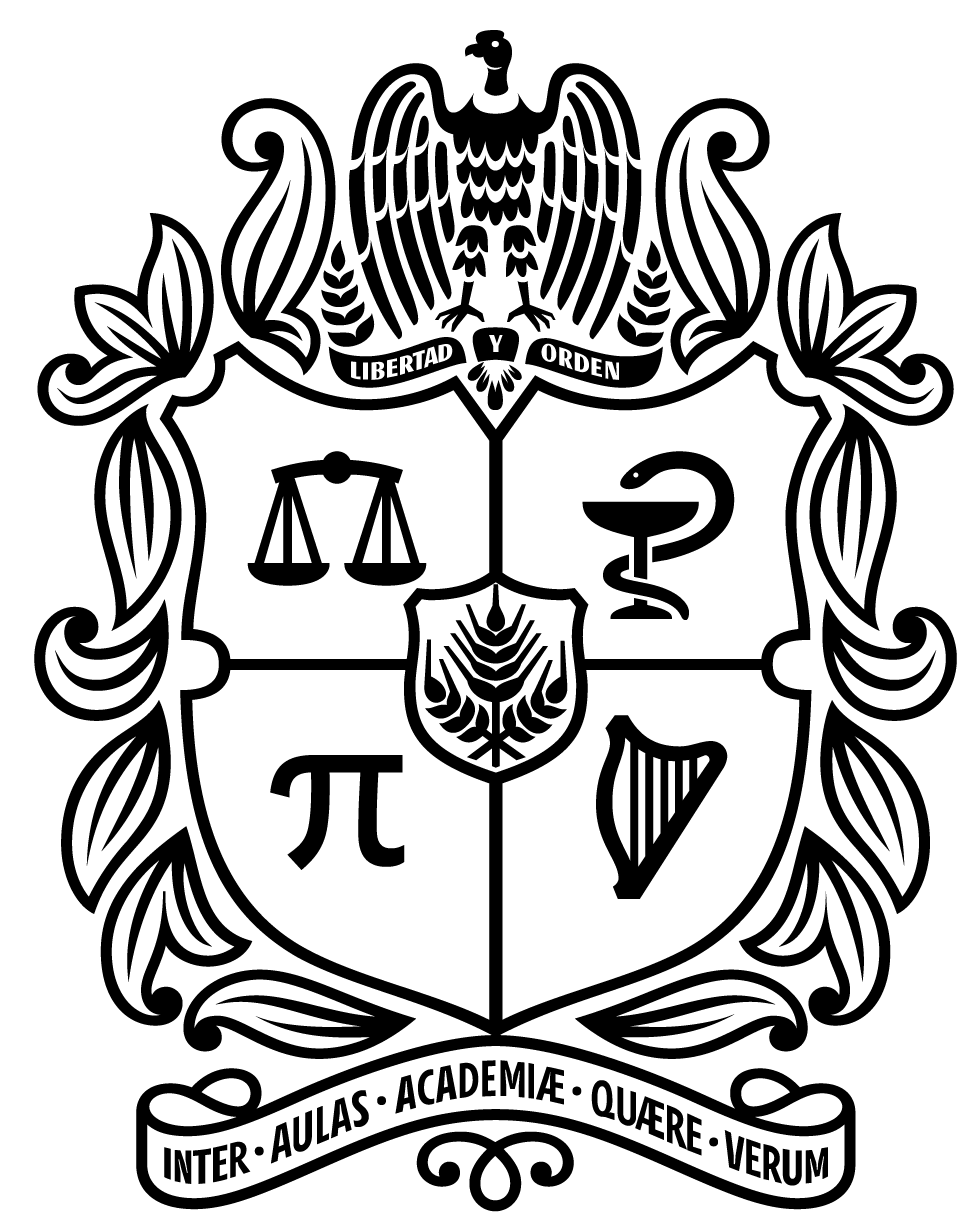
\includegraphics[width=0.55\paperwidth]
{Imágenes/escudo_marca_agua.png}
};

\end{tikzpicture}

\vspace*{\fill}

\begin{center}

{\color{verdeUN}\rule{3cm}{1.2pt}}

\vspace{1.2cm}

{\AncizarSansSemiBold
\fontsize{36}{42}\selectfont
\color{rojoUN}
#1 \thechapter}

\vspace{0.8cm}

{\AncizarSerifRegular
\fontsize{22}{28}\selectfont
#2}

\vspace{1.2cm}

{\color{verdeUN}\rule{3cm}{1.2pt}}

\end{center}

\vspace*{\fill}

\end{titlepage}

\addcontentsline{toc}{chapter}{#2}
}
\begin{titlepage}

%------------------------------------------------
% Barra lateral
%------------------------------------------------
\begin{tikzpicture}[remember picture,overlay]
    \fill[rojoUN]
    (current page.north west)
    rectangle
    ([xshift=3.2cm]current page.south west);
\end{tikzpicture}

%------------------------------------------------
% Encabezado
%------------------------------------------------

\hspace{3cm}
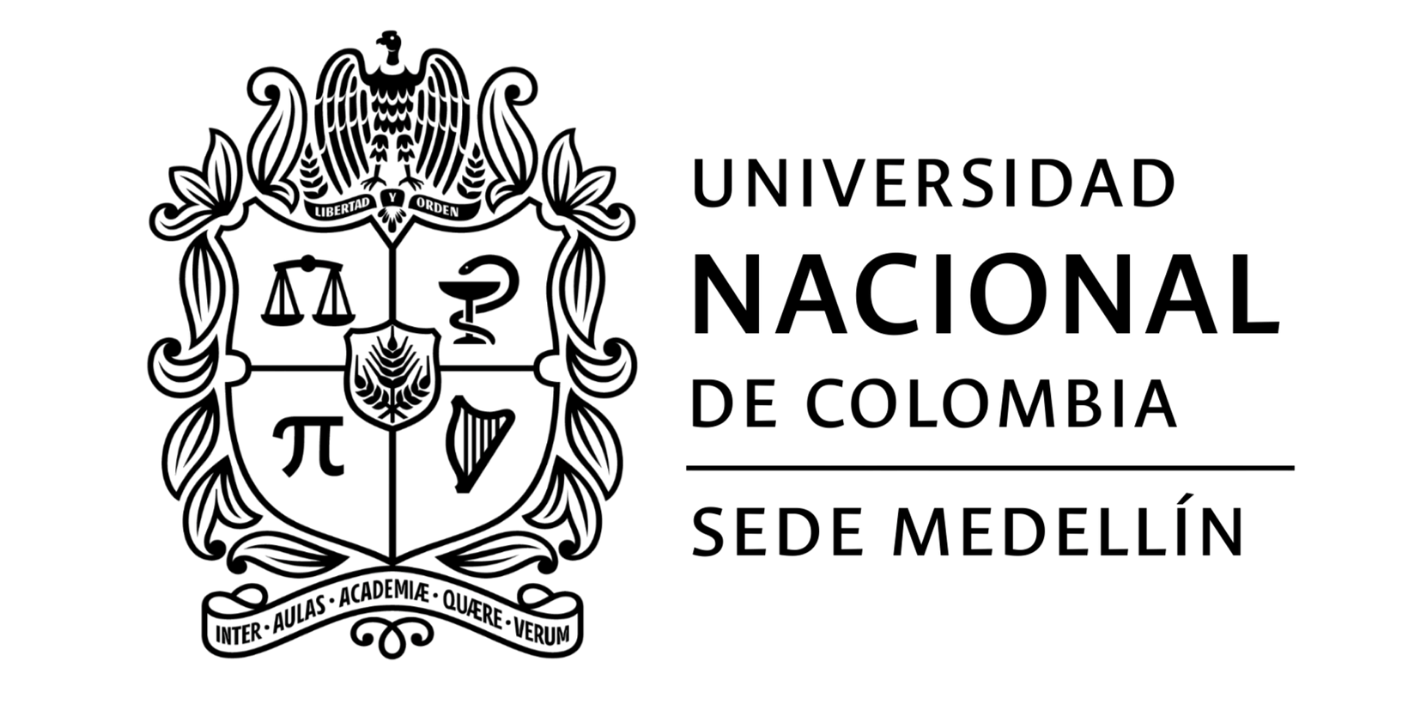
\includegraphics[width=0.6\textwidth]{Imágenes/logo_unal.png}

\vspace{0.8cm}

\hspace{4cm}
{\AncizarSansMedium\Large Departamento de Matemáticas}

\vspace{0.3cm}

\hspace{4cm}
{\color{verdeUN}\rule{3cm}{1.4pt}}

\vspace{2.4cm}

%------------------------------------------------
% Título
%------------------------------------------------

\hspace{4cm}
{\AncizarSansSemiBold\fontsize{34}{38}\selectfont
\color{rojoUN}
TALLER 1}

\vspace{0.45cm}

\hspace{4cm}
{\color{verdeUN}\rule{3cm}{1.4pt}}

\vspace{0.7cm}

\hspace{4cm}
{\AncizarSansMedium\fontsize{20}{24}\selectfont
Introducción a la Computación Cuántica}

\vspace{2.5cm}

%------------------------------------------------
% Autor
%------------------------------------------------

\hspace{4cm}
{\AncizarSansMedium\Large
María Paula Ardila Otero}

\vspace{1.5cm}

\hspace{4cm}
{\AncizarSansLightItalic\normalsize\color{rojoUN} Profesor}

\vspace{0.2cm}

\hspace{4cm}
{\AncizarSansRegular\Large
Johan Felipe Garcia Vargas}

\vfill

%------------------------------------------------
% Pie
%------------------------------------------------

\hspace{4cm}
{\color{verdeUN}\rule{3cm}{1.4pt}}

\vspace{0.35cm}

\hspace{4cm}
{\AncizarSansLightItalic\large
\today}

\end{titlepage}

\newpage

% Tabla de contenidos
\renewcommand{\contentsname}{Tabla de contenido}
\tableofcontents
\newpage


\color{rojoUN}

\section{Superposición, interferencia y la esfera de Bloch}

Sea $V = \text{span}_{\R}\{\cos(nt), \sin(nt) : n = 1,2\} \subset L^2([0, 2\pi])$. Para $A \ge 0$ y $x \in \R$, defina:
\begin{equation}
 (A e^{i x}) \cdot \cos(nt) = A \cos(nt - x), \quad n=1,2, 
 \label{eq:fase}
\end{equation}

e identifique $\ket{0} \leftrightarrow \cos(t)$, $\ket{1} \leftrightarrow \cos(2t)$.

\subsection{}

Demuestre que lo anterior hace de $V$ un espacio vectorial complejo de dimensión 2, y construya a partir del producto interno de $L^2$ un producto hermítico en el que $\{\ket{0}, \ket{1}\}$ sea ortonormal.

\color{Black}

\subsubsection*{Solución.}

\addcontentsline{toc}{subsubsection}{Solución.}

% ======================================================================
%  Taller 1 -- Punto 1.1 (cuerpo)
%  Requiere el bloque "preambulo_taller.tex" en el preámbulo.
%  Se puede pegar directamente en el documento o incluir con
%  \input{punto_1_1_cuerpo}.
% ======================================================================
% ====================== INICIO DEL PUNTO 1.1 ===========================



%======================================================================
\subsection*{El conjunto $V$}
%======================================================================

\begin{definicionT}[Combinación lineal y conjunto generado]
Dadas funciones $\varphi_1,\dots,\varphi_k$ definidas en $[0,2\pi]$, una
\emph{combinación lineal con coeficientes reales} de ellas es una función de la forma
$c_1\varphi_1+c_2\varphi_2+\dots+c_k\varphi_k$, con $c_1,\dots,c_k\in\mathbb R$. El conjunto de
todas estas combinaciones se llama \emph{conjunto generado} por $\varphi_1,\dots,\varphi_k$ y
se denota $\spanR\{\varphi_1,\dots,\varphi_k\}$.
\end{definicionT}

Según esta definición, los elementos de $V$ son las funciones de la forma
\begin{equation}\label{eq:forma-general}
  f(t) = a_1\Cu + b_1\Su + a_2\Cd + b_2\Sd,
  \qquad a_1, b_1, a_2, b_2 \in \mathbb{R}.
\end{equation}
En adelante, $a_n$ denota el coeficiente de $\cos nt$ y $b_n$ el de $\sin nt$. El subíndice
$n$ es la \emph{frecuencia} de la función, es decir, el número de oscilaciones completas que
realiza en el intervalo $[0,2\pi]$; así, $\Cu$ y $\Su$ tienen frecuencia $1$, y $\Cd$ y $\Sd$
tienen frecuencia $2$ (figura~\ref{fig:generadoras}). Todo elemento de $V$ es una función que
toma valores reales.

\begin{figure}[H]
\centering
\begin{tikzpicture}
\begin{axis}[ondaT, width=14cm, height=5.8cm,
  xtick={0,pi/4,pi/2,pi,3*pi/2,2*pi},
  xticklabels={$0$,$\frac{\pi}{4}$,$\frac{\pi}{2}$,$\pi$,$\frac{3\pi}{2}$,$2\pi$},
  legend style={at={(0.5,1.04)}, anchor=south, legend columns=4, draw=none,
                font=\small, column sep=8pt},
  ]
  \addplot[very thick, colCu] {cos(x)};    \addlegendentry{$\cos t$}
  \addplot[very thick, colSu] {sin(x)};    \addlegendentry{$\sin t$}
  \addplot[very thick, colCd] {cos(2*x)};  \addlegendentry{$\cos 2t$}
  \addplot[very thick, colSd] {sin(2*x)};  \addlegendentry{$\sin 2t$}
  \draw[dashed, black!50] (axis cs:0.7854,-1.25) -- (axis cs:0.7854,1.25);
  \draw[dashed, black!50] (axis cs:1.5708,-1.25) -- (axis cs:1.5708,1.25);
  \draw[dashed, black!50] (axis cs:3.1416,-1.25) -- (axis cs:3.1416,1.25);
\end{axis}
\end{tikzpicture}
\caption{Las cuatro funciones que generan $V$. Las de frecuencia $1$ completan una oscilación
en $[0,2\pi]$ y las de frecuencia $2$ completan dos. Las líneas punteadas marcan los puntos
$t=\pi/4,\ \pi/2,\ \pi$ que, junto con $t=0$, se usan en la demostración del
lema~\ref{lema:independencia}.}
\label{fig:generadoras}
\end{figure}

\begin{definicionT}[Independencia lineal sobre $\mathbb R$]
Las funciones $\varphi_1,\dots,\varphi_k$ son \emph{linealmente independientes sobre
$\mathbb R$} si la única combinación lineal con coeficientes reales que da la función cero (la
que vale $0$ en todo $t$) es aquella con todos sus coeficientes iguales a cero; es decir, si
\[
  c_1\varphi_1(t)+\dots+c_k\varphi_k(t)=0 \ \text{ para todo } t\in[0,2\pi]
  \quad\Longrightarrow\quad c_1=\dots=c_k=0 .
\]
\end{definicionT}

\begin{lemaT}{lema:independencia}
Las funciones $\cos t$, $\sin t$, $\cos 2t$ y $\sin 2t$ son linealmente independientes sobre
$\mathbb R$. En consecuencia, si dos expresiones de la forma $f(t)=a_1\cos t+b_1\sin t+a_2\cos 2t+b_2\sin 2t$ \eqref{eq:forma-general}
representan la misma función, sus coeficientes coinciden.
\end{lemaT}

\begin{proof}
Supóngase que
\begin{equation}\label{eq:combinacion-cero}
  a_1\cos t + b_1\sin t + a_2\cos 2t + b_2\sin 2t = 0
  \qquad\text{para todo } t\in[0,2\pi].
\end{equation}
Como la igualdad se cumple para todo $t$, se cumple en particular en los puntos donde varias
de las cuatro funciones valen $0$ o $\pm 1$, que son los marcados en la
figura~\ref{fig:generadoras}. Los valores en esos puntos son
\[
\begin{array}{c|cccc}
 t & \cos t & \sin t & \cos 2t & \sin 2t\\ \hline
 0 & 1 & 0 & 1 & 0\\
 \pi/4 & \tfrac{\sqrt2}{2} & \tfrac{\sqrt2}{2} & 0 & 1\\
 \pi/2 & 0 & 1 & -1 & 0\\
 \pi & -1 & 0 & 1 & 0
\end{array}
\]
Al evaluar $a_1\cos t+b_1\sin t+a_2\cos 2t+b_2\sin 2t=0$ \eqref{eq:combinacion-cero} en $t=0$ y en $t=\pi$ se obtienen las ecuaciones
$a_1+a_2=0$ y $-a_1+a_2=0$. Sumándolas resulta $2a_2=0$, es decir, $a_2=0$, y entonces
$a_1=0$. Al evaluar en $t=\pi/2$ se obtiene $b_1-a_2=0$, y como $a_2=0$, también $b_1=0$.
Finalmente, al evaluar en $t=\pi/4$ queda
$\tfrac{\sqrt2}{2}a_1+\tfrac{\sqrt2}{2}b_1+b_2=0$, y como $a_1=b_1=0$, resulta $b_2=0$. Así,
los cuatro coeficientes son cero.

Para la segunda afirmación, supóngase que una misma función $f$ se escribe con coeficientes
$a_1,b_1,a_2,b_2$ y también con coeficientes $\tilde a_1,\tilde b_1,\tilde a_2,\tilde b_2$. Al
restar ambas expresiones se obtiene
$(a_1-\tilde a_1)\cos t+(b_1-\tilde b_1)\sin t+(a_2-\tilde a_2)\cos 2t+(b_2-\tilde b_2)\sin 2t=0$
para todo $t$, y por la primera parte cada diferencia es cero, es decir, $a_1=\tilde a_1$,
$b_1=\tilde b_1$, $a_2=\tilde a_2$ y $b_2=\tilde b_2$.
\end{proof}

Gracias al lema tiene sentido hablar de \emph{los} coeficientes de un elemento de $V$, y dos
elementos de $V$ son iguales exactamente cuando sus cuatro coeficientes coinciden. Este es el
criterio que se usa en todas las verificaciones siguientes.

%======================================================================
\subsection*{Propiedades de espacio vectorial complejo}
%======================================================================

\begin{definicionT}[Espacio vectorial complejo]
Un conjunto $V$ es un \emph{espacio vectorial complejo} si tiene definidas dos operaciones, la
suma $f+g$ de dos elementos y la multiplicación $z\cdot f$ de un elemento por un número
complejo $z$, cuyos resultados pertenecen otra vez a $V$ y que cumplen las
siguientes propiedades para todo $f, g, h\in V$ y todo $z, w\in\mathbb{C}$.

\smallskip
\noindent\textbf{Propiedades de la suma.}
\begin{enumerate}
  \item[(S1)] $f+g = g+f$.
  \item[(S2)] $(f+g)+h = f+(g+h)$.
  \item[(S3)] Existe un elemento $0\in V$ tal que $f+0 = f$.
  \item[(S4)] Para cada $f$ existe $-f\in V$ tal que $f+(-f) = 0$.
\end{enumerate}
\noindent\textbf{Propiedades de la multiplicación por escalares.}
\begin{enumerate}
  \item[(M1)] $z\cdot(f+g) = z\cdot f + z\cdot g$.
  \item[(M2)] $(z+w)\cdot f = z\cdot f + w\cdot f$.
  \item[(M3)] $(zw)\cdot f = z\cdot(w\cdot f)$.
  \item[(M4)] $1\cdot f = f$.
\end{enumerate}
\end{definicionT}

En $V$ la suma es la suma usual de funciones, $(f+g)(t)=f(t)+g(t)$, mientras que la
multiplicación por escalares complejos se construye a partir de la regla del enunciado. Las dos
operaciones se estudian por separado.

\subsubsection*{La suma}

Sean $f, g, h\in V$. Por la definición de $V$, existen números reales
$a_1, b_1, a_2, b_2$, $a_1', b_1', a_2', b_2'$ y $a_1'', b_1'', a_2'', b_2''$ tales que
\begin{align*}
  f &= a_1\cos t + b_1\sin t + a_2\cos 2t + b_2\sin 2t,\\
  g &= a_1'\cos t + b_1'\sin t + a_2'\cos 2t + b_2'\sin 2t,\\
  h &= a_1''\cos t + b_1''\sin t + a_2''\cos 2t + b_2''\sin 2t.
\end{align*}

\paragraph{La suma pertenece a $V$.}
Al sumar $f$ y $g$ y agrupar los términos que contienen la misma función, se obtiene
\begin{equation}\label{eq:suma}
  f+g = (a_1+a_1')\cos t + (b_1+b_1')\sin t + (a_2+a_2')\cos 2t + (b_2+b_2')\sin 2t.
\end{equation}
Como $a_1+a_1'$, $b_1+b_1'$, $a_2+a_2'$ y $b_2+b_2'$ son números reales, $f+g$ es de la
forma $f(t)=a_1\cos t+b_1\sin t+a_2\cos 2t+b_2\sin 2t$ \eqref{eq:forma-general} y por tanto pertenece a $V$. En otras palabras, sumar dos
elementos de $V$ equivale a sumar sus coeficientes uno a uno.

\paragraph{(S1) $f+g = g+f$.}
Por $f+g=(a_1+a_1')\cos t+(b_1+b_1')\sin t+(a_2+a_2')\cos 2t+(b_2+b_2')\sin 2t$ \eqref{eq:suma}, los coeficientes de $f+g$ son $a_1+a_1'$, $b_1+b_1'$, $a_2+a_2'$ y
$b_2+b_2'$, mientras que los de $g+f$ son $a_1'+a_1$, $b_1'+b_1$, $a_2'+a_2$ y $b_2'+b_2$. Como
la suma de números reales no depende del orden, $a_1+a_1'=a_1'+a_1$, y lo mismo ocurre con los
otros tres coeficientes. Al tener los mismos coeficientes, $f+g=g+f$.

\paragraph{(S2) $(f+g)+h = f+(g+h)$.}
Al aplicar $f+g=(a_1+a_1')\cos t+(b_1+b_1')\sin t+(a_2+a_2')\cos 2t+(b_2+b_2')\sin 2t$ \eqref{eq:suma} dos veces, el coeficiente de $\cos t$ en $(f+g)+h$ es
$(a_1+a_1')+a_1''$ y en $f+(g+h)$ es $a_1+(a_1'+a_1'')$. Estos números son iguales porque la
suma de números reales es asociativa. El mismo argumento se aplica a los coeficientes de
$\sin t$, $\cos 2t$ y $\sin 2t$, de modo que $(f+g)+h = f+(g+h)$.

\paragraph{(S3) Existe $0\in V$ tal que $f+0 = f$.}
Sea $0$ la función con sus cuatro coeficientes iguales a cero,
\[
  0 = 0\cos t + 0\sin t + 0\cos 2t + 0\sin 2t,
\]
que pertenece a $V$ porque $0$ es un número real; se trata de la función que vale $0$ en todo
$t$. Por $f+g=(a_1+a_1')\cos t+(b_1+b_1')\sin t+(a_2+a_2')\cos 2t+(b_2+b_2')\sin 2t$ \eqref{eq:suma},
\[
  f+0 = (a_1+0)\cos t + (b_1+0)\sin t + (a_2+0)\cos 2t + (b_2+0)\sin 2t = f.
\]

\paragraph{(S4) Para cada $f$ existe $-f\in V$ tal que $f+(-f) = 0$.}
Sea $-f$ la función con los coeficientes de $f$ cambiados de signo,
\[
  -f = (-a_1)\cos t + (-b_1)\sin t + (-a_2)\cos 2t + (-b_2)\sin 2t,
\]
que pertenece a $V$ porque $-a_1, -b_1, -a_2, -b_2$ son números reales. Por $f+g=(a_1+a_1')\cos t+(b_1+b_1')\sin t+(a_2+a_2')\cos 2t+(b_2+b_2')\sin 2t$ \eqref{eq:suma},
\[
  f+(-f) = (a_1-a_1)\cos t + (b_1-b_1)\sin t + (a_2-a_2)\cos 2t + (b_2-b_2)\sin 2t = 0.
\]
Con esto, la suma en $V$ produce elementos de $V$ y cumple (S1)--(S4).

\subsubsection*{La multiplicación por escalares complejos}

La regla del enunciado está escrita en términos de la forma polar de un número complejo, por
lo que conviene fijar primero la notación correspondiente.

\begin{definicionT}[Partes, conjugado y módulo de un número complejo]
Todo número complejo se escribe como $z=a+ib$, con $a,b\in\mathbb R$ e $i^2=-1$. El número
$a=\Real z$ es su \emph{parte real} y $b=\Imag z$ su \emph{parte imaginaria}. El
\emph{conjugado} de $z$ es $\overline z=a-ib$ y su \emph{módulo} es $|z|=\sqrt{a^2+b^2}$. Al
multiplicar $z$ por su conjugado se obtiene
\begin{equation}\label{eq:modulo}
  z\,\overline z=(a+ib)(a-ib)=a^2-i^2b^2=a^2+b^2=|z|^2 .
\end{equation}
El conjugado respeta la suma y el producto y, al aplicarse dos veces, devuelve el número
original: para $z,w\in\mathbb C$,
\begin{equation}\label{eq:conjugado}
  \overline{z+w}=\overline z+\overline w,\qquad
  \overline{zw}=\overline z\,\overline w,\qquad
  \overline{\overline z}=z .
\end{equation}
Estas igualdades se comprueban escribiendo $z=a+ib$, $w=c+id$ y desarrollando ambos lados.
\end{definicionT}

\begin{definicionT}[Forma polar]
La \emph{fórmula de Euler} establece que, para $x\in\mathbb R$,
$e^{ix}=\cos x+i\sin x$. Todo número complejo $z=a+ib$ puede escribirse en \emph{forma polar}
$z=Ae^{ix}$, donde $A=|z|\ge 0$ es su módulo y $x$ es el ángulo que forma el segmento que va
de $0$ a $z$ con el eje real. Leyendo la figura como un triángulo
rectángulo de hipotenusa $A$, se tiene
\begin{equation}\label{eq:polar}
  a=A\cos x,\qquad b=A\sin x .
\end{equation}
El ángulo $x$ no es único: $x$ y $x+2\pi$ describen el mismo número, y si $z=0$ cualquier
ángulo sirve.
\end{definicionT}


\paragraph{Significado de la regla.}
La regla del enunciado,
\[
  (Ae^{ix})\cdot\cos nt = A\cos(nt-x),\qquad n=1,2,
\]
tiene una lectura gráfica directa. Como $A\cos(nt-x)=A\cos\bigl(n(t-x/n)\bigr)$, la función
resultante es la gráfica de $\cos nt$ desplazada $x/n$ unidades hacia la derecha y estirada
verticalmente por el factor $A$. El módulo del número complejo controla la altura de la onda y
el ángulo controla su posición.

\paragraph{La regla en términos de las partes real e imaginaria.}
Sea $z=a+ib\in\mathbb C$ escrito en forma polar como $z=Ae^{ix}$. Al aplicar la regla, usar la
fórmula del coseno de una resta, $\cos(nt-x)=\cos nt\cos x+\sin nt\sin x$, y luego
$a=A\cos x,\quad\penalty0 b=A\sin x$ \eqref{eq:polar}, se obtiene
\begin{align*}
  (a+ib)\cdot\cos nt
  &=A\cos(nt-x)
   =A\bigl(\cos nt\cos x+\sin nt\sin x\bigr)\\
  &=(A\cos x)\cos nt+(A\sin x)\sin nt
   =a\cos nt+b\sin nt .
\end{align*}
Por tanto,
\begin{equation}\label{eq:regla-coef}
  \destacado{(a+ib)\cdot\cos nt=a\cos nt+b\sin nt,\qquad n=1,2.}
\end{equation}
El lado derecho depende únicamente de $a$ y $b$, no del ángulo $x$ elegido, así que la regla
asigna una sola función a cada número complejo aunque su forma polar no sea única. Además, si
$z=a$ es real ($b=0$), la regla da $a\cdot\cos nt=a\cos nt$, que es el producto usual de un
número real por una función; la nueva multiplicación extiende, por tanto, la multiplicación
por números reales. En el caso particular $z=i$, es decir, $a=0$ y $b=1$, la fórmula
$(a+ib)\cdot\cos nt=a\cos nt+b\sin nt$ \eqref{eq:regla-coef} da
\begin{equation}\label{eq:i-cos}
  i\cdot\cos nt=\sin nt ,
\end{equation}
que es lo que muestra en la figura~\ref{fig:regla}.

\begin{figure}[H]
\centering
\begin{tikzpicture}
\begin{axis}[ondaT, title={$i\cdot\cos t=\cos(t-\pi/2)=\sin t$}]
  \addplot[very thick, colCu] {cos(x)};
  \addplot[very thick, colSu] {sin(x)};
  \draw[-{Stealth[length=2mm]}, thick] (axis cs:0,1.2) -- (axis cs:1.5708,1.2)
     node[midway, above, font=\footnotesize] {$\pi/2$};
  \node[colCu, font=\footnotesize] at (axis cs:5.75,1.15) {$\cos t$};
  \node[colSu, font=\footnotesize] at (axis cs:4.0,-1.2) {$\sin t$};
\end{axis}
\end{tikzpicture}
\caption{}
\label{fig:regla}
\end{figure}

\paragraph{Coordenadas complejas de un elemento de $V$.}
La regla solo indica cómo multiplicar $\cos t$ y $\cos 2t$ por un número complejo; para
multiplicar un elemento cualquiera de $V$ hace falta extenderla. La fórmula
$(a+ib)\cdot\cos nt=a\cos nt+b\sin nt$ \eqref{eq:regla-coef}, leída de derecha a izquierda, muestra cómo hacerlo, pues dice que una
pareja de términos con la misma frecuencia es un múltiplo complejo de $\cos nt$:
\[
  a_1\cos t+b_1\sin t=(a_1+ib_1)\cdot\cos t,
  \qquad
  a_2\cos 2t+b_2\sin 2t=(a_2+ib_2)\cdot\cos 2t .
\]

\begin{definicionT}[Coordenadas complejas]
Para $f\in V$ con coeficientes $a_1,b_1,a_2,b_2$ como en $f(t)=a_1\cos t+b_1\sin t+a_2\cos 2t+b_2\sin 2t$ \eqref{eq:forma-general}, sus
\emph{coordenadas complejas} son los números
\[
  \alpha=a_1+ib_1,\qquad \beta=a_2+ib_2 .
\]
La parte real de $\alpha$ es el coeficiente de $\cos t$ y su parte imaginaria es el
coeficiente de $\sin t$; lo mismo ocurre con $\beta$ para la frecuencia $2$.
\end{definicionT}

Con esta notación, todo elemento de $V$ se escribe como
\begin{equation}\label{eq:alfa-beta}
  f=\alpha\cdot\Cu+\beta\cdot\Cd .
\end{equation}
Por el lema~\ref{lema:independencia}, los números $\alpha$ y $\beta$ quedan determinados por
$f$ de manera única, y cada pareja $(\alpha,\beta)$ corresponde a una única función de $V$.
Del mismo modo, las coordenadas complejas de $g$ y $h$ se denotan
$\alpha'=a_1'+ib_1'$, $\beta'=a_2'+ib_2'$ y $\alpha''=a_1''+ib_1''$, $\beta''=a_2''+ib_2''$.

La suma también se describe en estas coordenadas. Por $f+g=(a_1+a_1')\cos t+(b_1+b_1')\sin t+(a_2+a_2')\cos 2t+(b_2+b_2')\sin 2t$ \eqref{eq:suma}, los coeficientes de
$\cos t$ y $\sin t$ en $f+g$ son $a_1+a_1'$ y $b_1+b_1'$, así que su primera coordenada
compleja es $(a_1+a_1')+i(b_1+b_1')=\alpha+\alpha'$; de la misma forma, la segunda es
$\beta+\beta'$. Es decir,
\begin{equation}\label{eq:suma-coord}
  f+g=(\alpha+\alpha')\cdot\cos t+(\beta+\beta')\cdot\cos 2t ,
\end{equation}
y sumar en $V$ equivale a sumar las coordenadas complejas una a una.

\paragraph{Definición de la multiplicación.}
Para $z\in\mathbb C$ y $f=\alpha\cdot\cos t+\beta\cdot\cos 2t$ se define
\begin{equation}\label{eq:mult}
  \destacado{z\cdot f=(z\alpha)\cdot\cos t+(z\beta)\cdot\cos 2t ,}
\end{equation}
es decir, multiplicar $f$ por $z$ consiste en multiplicar por $z$ cada una de sus coordenadas
complejas. La definición no presenta ambigüedad, porque $\alpha$ y $\beta$ son únicos, y es
compatible con el enunciado: para $f=\cos t$ se tiene $\alpha=1$, $\beta=0$, y
$z\cdot f=(z\alpha)\cdot\cos t+(z\beta)\cdot\cos 2t$ \eqref{eq:mult} se reduce a $z\cdot\cos t$ tal como lo da la regla; lo mismo ocurre con
$\cos 2t$. Además, el resultado pertenece a $V$: si $z\alpha=p+iq$ con $p,q\in\mathbb R$, por
$(a+ib)\cdot\cos nt=a\cos nt+b\sin nt$ \eqref{eq:regla-coef} se tiene $(z\alpha)\cdot\cos t=p\cos t+q\sin t$, y análogamente para
$z\beta$, de modo que $z\cdot f$ es una combinación con coeficientes reales de las cuatro
funciones generadoras.

\paragraph{Multiplicación por $i$.}
Este caso se usa de nuevo en la construcción del producto hermítico. Como
$i\alpha=i(a_1+ib_1)=-b_1+ia_1$ e $i\beta=-b_2+ia_2$, la definición $z\cdot f=(z\alpha)\cdot\cos t+(z\beta)\cdot\cos 2t$ \eqref{eq:mult} junto con
$(a+ib)\cdot\cos nt=a\cos nt+b\sin nt$ \eqref{eq:regla-coef} da
\begin{equation}\label{eq:i-f}
  \destacado{i\cdot f=-b_1\cos t+a_1\sin t-b_2\cos 2t+a_2\sin 2t .}
\end{equation}
En particular, $\sin nt$ tiene coordenada compleja $i$ (porque $\sin nt=i\cdot\cos nt$ por
$i\cdot\cos nt=\sin nt$ \eqref{eq:i-cos}), así que $i\cdot\sin nt=(i\cdot i)\cdot\cos nt=-\cos nt$. Multiplicar por
$i$ desplaza cada onda un cuarto de período: $\cos nt$ pasa a $\sin nt$ y $\sin nt$ pasa a
$-\cos nt$.

\paragraph{(M1) $z\cdot(f+g)=z\cdot f+z\cdot g$.}
Por $f+g=(\alpha+\alpha')\cdot\cos t+(\beta+\beta')\cdot\cos 2t$ \eqref{eq:suma-coord}, $f+g$ tiene coordenadas $\alpha+\alpha'$ y $\beta+\beta'$, y por
$z\cdot f=(z\alpha)\cdot\cos t+(z\beta)\cdot\cos 2t$ \eqref{eq:mult},
\[
  z\cdot(f+g)=\bigl(z(\alpha+\alpha')\bigr)\cdot\cos t
  +\bigl(z(\beta+\beta')\bigr)\cdot\cos 2t .
\]
Por otra parte, $z\cdot f$ tiene coordenadas $z\alpha$, $z\beta$ y $z\cdot g$ tiene
coordenadas $z\alpha'$, $z\beta'$, de modo que, por $f+g=(\alpha+\alpha')\cdot\cos t+(\beta+\beta')\cdot\cos 2t$ \eqref{eq:suma-coord},
\[
  z\cdot f+z\cdot g=(z\alpha+z\alpha')\cdot\cos t+(z\beta+z\beta')\cdot\cos 2t .
\]
La multiplicación de números complejos se distribuye sobre la suma, así que
$z(\alpha+\alpha')=z\alpha+z\alpha'$ y $z(\beta+\beta')=z\beta+z\beta'$. Ambos lados tienen las
mismas coordenadas y, por tanto, $z\cdot(f+g)=z\cdot f+z\cdot g$.

\paragraph{(M2) $(z+w)\cdot f=z\cdot f+w\cdot f$.}
Por $z\cdot f=(z\alpha)\cdot\cos t+(z\beta)\cdot\cos 2t$ \eqref{eq:mult}, las coordenadas de $(z+w)\cdot f$ son $(z+w)\alpha$ y $(z+w)\beta$. Por
$z\cdot f=(z\alpha)\cdot\cos t+(z\beta)\cdot\cos 2t$ \eqref{eq:mult} y $f+g=(\alpha+\alpha')\cdot\cos t+(\beta+\beta')\cdot\cos 2t$ \eqref{eq:suma-coord}, las de $z\cdot f+w\cdot f$ son $z\alpha+w\alpha$ y
$z\beta+w\beta$. Por la propiedad distributiva en $\mathbb C$, $(z+w)\alpha=z\alpha+w\alpha$ y
$(z+w)\beta=z\beta+w\beta$, de modo que las coordenadas coinciden y
$(z+w)\cdot f=z\cdot f+w\cdot f$.

\paragraph{(M3) $(zw)\cdot f=z\cdot(w\cdot f)$.}
Las coordenadas de $(zw)\cdot f$ son $(zw)\alpha$ y $(zw)\beta$. Por otro lado, $w\cdot f$ tiene
coordenadas $w\alpha$ y $w\beta$, y al multiplicar por $z$ se obtienen $z(w\alpha)$ y
$z(w\beta)$. Como la multiplicación de números complejos es asociativa,
$(zw)\alpha=z(w\alpha)$ y $(zw)\beta=z(w\beta)$, de donde $(zw)\cdot f=z\cdot(w\cdot f)$.

\paragraph{(M4) $1\cdot f=f$.}
Con $z=1$, la definición $z\cdot f=(z\alpha)\cdot\cos t+(z\beta)\cdot\cos 2t$ \eqref{eq:mult} da
$1\cdot f=(1\alpha)\cdot\cos t+(1\beta)\cdot\cos 2t=\alpha\cdot\cos t+\beta\cdot\cos 2t=f$.

\medskip
Así, la multiplicación por escalares complejos produce elementos de $V$ y se cumplen (M1)--(M4). Junto
con lo demostrado para la suma, esto prueba que $V$ es un espacio vectorial complejo.

%======================================================================
\subsection*{Dimensión compleja de $V$}
%======================================================================

\begin{definicionT}[Base y dimensión]
Un conjunto $\{v_1,\dots,v_k\}$ de vectores de un espacio vectorial complejo $V$ es una
\emph{base} de $V$ si cumple dos condiciones. La primera es que \emph{genera} $V$: todo
vector de $V$ se escribe como $c_1\cdot v_1+\dots+c_k\cdot v_k$ con $c_1,\dots,c_k\in\mathbb C$.
La segunda es que es \emph{linealmente independiente sobre $\mathbb C$}: si
$c_1\cdot v_1+\dots+c_k\cdot v_k=0$ con $c_j\in\mathbb C$, entonces $c_1=\dots=c_k=0$. Todas
las bases de un mismo espacio tienen el mismo número de elementos, y ese número se llama
\emph{dimensión} del espacio; para un espacio complejo se denota $\dim_{\mathbb C}V$.
\end{definicionT}

El conjunto $\{\cos t,\cos 2t\}$ genera $V$, pues por $f=\alpha\cdot\cos t+\beta\cdot\cos 2t$ \eqref{eq:alfa-beta} todo elemento de $V$
se escribe como $\alpha\cdot\cos t+\beta\cdot\cos 2t$ con $\alpha,\beta\in\mathbb C$. Para la
independencia, supóngase que $\alpha\cdot\cos t+\beta\cdot\cos 2t=0$ con
$\alpha=a_1+ib_1$ y $\beta=a_2+ib_2$. Por $(a+ib)\cdot\cos nt=a\cos nt+b\sin nt$ \eqref{eq:regla-coef}, el lado izquierdo es la función
$a_1\cos t+b_1\sin t+a_2\cos 2t+b_2\sin 2t$, que es la función cero; por el
lema~\ref{lema:independencia}, $a_1=b_1=a_2=b_2=0$, es decir, $\alpha=\beta=0$. En
consecuencia, $\{\cos t,\cos 2t\}$ es una base de $V$ y
\[
  \destacado{\dim_{\mathbb C}V=2 .}
\]

\begin{definicionT}[Notación de Dirac]
En computación cuántica, los vectores del espacio de estados se escriben con el símbolo
$\ket{\psi}$, llamado \emph{ket}, donde $\psi$ es solo un nombre. Siguiendo el enunciado, se
denota
\[
  \ket0=\cos t,\qquad \ket1=\cos 2t .
\]
\end{definicionT}

Con esta notación, $f=\alpha\cdot\cos t+\beta\cdot\cos 2t$ \eqref{eq:alfa-beta} se escribe $f=\alpha\ket0+\beta\ket1$, y el resultado
anterior dice que $V=\spanC\{\ket0,\ket1\}$, donde $\spanC$ indica combinaciones lineales con
coeficientes complejos.


%======================================================================
\subsection*{El producto interno de $L^2$ en $V$}
%======================================================================

\begin{definicionT}[El espacio $L^2$ y su producto interno]
El espacio $L^2([0,2\pi])$ está formado por las funciones definidas en $[0,2\pi]$ cuyo
cuadrado tiene integral finita en ese intervalo. Para dos funciones reales $f,g$ de este
espacio, su \emph{producto interno de $L^2$} es
\[
  \destacado{\Lp fg=\int_0^{2\pi}f(t)\,g(t)\,dt .}
\]
Para funciones con valores complejos aparece además un conjugado en uno de los factores, pero
todos los elementos de $V$ son funciones reales, de modo que ese conjugado no interviene aquí.
El subíndice $L^2$ indica el espacio del que proviene el producto, y los paréntesis lo
distinguen del producto hermítico $\bk fg$ que se construye más adelante.
\end{definicionT}

Los elementos de $V$ pertenecen a $L^2([0,2\pi])$ porque son funciones continuas en un
intervalo cerrado y acotado. El producto $\Lp fg$ es un número real y es simétrico,
$\Lp fg=\Lp gf$, porque $f(t)g(t)=g(t)f(t)$. Además, como la integral de una suma es la suma de
las integrales y las constantes salen de la integral, es lineal en cada argumento: para
$c,d\in\mathbb R$,
\begin{equation}\label{eq:L2-lineal}
  \Lp{cf+dg}{h}=c\,\Lp fh+d\,\Lp gh,
  \qquad
  \Lp{f}{cg+dh}=c\,\Lp fg+d\,\Lp fh .
\end{equation}
Las constantes que salen de este producto son números \emph{reales}, y esa restricción es la
que obliga más adelante a modificarlo.

\paragraph{Reducción a productos de senos y cosenos.}
Para calcular $\Lp fg$ con $f$ y $g$ arbitrarios en $V$ se vuelve a su escritura
$f(t)=a_1\cos t+b_1\sin t+a_2\cos 2t+b_2\sin 2t$ \eqref{eq:forma-general}. Para abreviar, las cuatro funciones generadoras se nombran
\[
  \varphi_1=\Cu,\qquad \varphi_2=\Su,\qquad \varphi_3=\Cd,\qquad \varphi_4=\Sd,
\]
y los coeficientes de $f$ y $g$ se agrupan como
$(c_1,c_2,c_3,c_4)=(a_1,b_1,a_2,b_2)$ y $(c_1',c_2',c_3',c_4')=(a_1',b_1',a_2',b_2')$, de modo
que $f=\sum_{j=1}^4 c_j\varphi_j$ y $g=\sum_{k=1}^4 c_k'\varphi_k$. Por la linealidad
$(cf+dg,h)_{L^2}=c\,(f,h)_{L^2}+d\,(g,h)_{L^2},\quad\penalty0 (f,cg+dh)_{L^2}=c\,(f,g)_{L^2}+d\,(f,h)_{L^2}$ \eqref{eq:L2-lineal}, los coeficientes salen del producto:
\begin{equation}\label{eq:L2-expansion}
  \Lp fg=\int_0^{2\pi}\Bigl(\sum_{j=1}^4 c_j\varphi_j(t)\Bigr)\Bigl(\sum_{k=1}^4 c_k'\varphi_k(t)\Bigr)dt
  =\sum_{j=1}^4\sum_{k=1}^4 c_j\,c_k'\,\Lp{\varphi_j}{\varphi_k} .
\end{equation}
Calcular el producto de dos elementos cualesquiera de $V$ se reduce entonces a conocer los
dieciséis productos $\Lp{\varphi_j}{\varphi_k}$ entre las cuatro funciones con las que se
construyen $f$ y $g$. Cada uno es la integral de un producto de dos funciones
trigonométricas, de la forma $\cos(nt)\cos(mt)$, $\sin(nt)\sin(mt)$ o $\cos(nt)\sin(mt)$ con
$n,m\in\{1,2\}$; esa es la razón por la que a continuación se trabaja con productos de senos y
cosenos.

\paragraph{Identidades de producto a suma.}
Un producto de dos funciones trigonométricas no se integra de forma directa, pero puede
reescribirse como una suma de un solo coseno o un solo seno, cuya integral es inmediata. Para
ello se parte de las fórmulas de suma y resta de ángulos,
\begin{align*}
\cos(A-B) &= \cos A\cos B + \sin A\sin B, & \cos(A+B) &= \cos A\cos B - \sin A\sin B,\\
\sin(A+B) &= \sin A\cos B + \cos A\sin B, & \sin(A-B) &= \sin A\cos B - \cos A\sin B.
\end{align*}
Al sumar las dos primeras se cancela $\sin A\sin B$; al restarlas se cancela
$\cos A\cos B$; y al restar la cuarta de la tercera se cancela $\sin A\cos B$. Despejando, y
tomando $A=nt$, $B=mt$, se obtiene
\begin{equation}\label{eq:producto-suma}
\begin{aligned}
\cos(nt)\cos(mt) &= \tfrac12\bigl[\cos((n-m)t) + \cos((n+m)t)\bigr],\\
\sin(nt)\sin(mt) &= \tfrac12\bigl[\cos((n-m)t) - \cos((n+m)t)\bigr],\\
\cos(nt)\sin(mt) &= \tfrac12\bigl[\sin((n+m)t) - \sin((n-m)t)\bigr].
\end{aligned}
\end{equation}
Después de aplicar estas identidades, solo quedan por calcular integrales de la forma
$\int_0^{2\pi}\cos(kt)\,dt$ y $\int_0^{2\pi}\sin(kt)\,dt$ con $k$ entero.

\paragraph{Integral de un solo coseno o un solo seno.}
La figura~\ref{fig:integrales} muestra por qué estas integrales valen cero cuando $k\ne 0$. En
$[0,2\pi]$, la función $\cos(kt)$ o $\sin(kt)$ completa exactamente $k$ oscilaciones, y en cada
oscilación el tramo de curva que queda por encima del eje encierra la misma área que el que
queda por debajo, pues uno es el reflejo del otro. Los ceros de la función separan esos tramos:
$\cos t$ se anula en $\pi/2$ y $3\pi/2$; $\cos 2t$ en $\pi/4$, $3\pi/4$, $5\pi/4$ y $7\pi/4$;
$\sin t$ en $0$, $\pi$ y $2\pi$; y $\sin 2t$ en $0$, $\pi/2$, $\pi$, $3\pi/2$ y $2\pi$. Como la
integral cuenta con signo positivo el área por encima del eje y con signo negativo el área
por debajo, las dos contribuciones se cancelan.

\begin{figure}[H]
\centering
\panelarea{cos(x)}{colCu}{$\cos t$}{(1.5708,0) (4.7124,0)}{
  \node[font=\small] at (axis cs:0.6,0.35) {$+$};
  \node[font=\small] at (axis cs:3.1416,-0.4) {$-$};
  \node[font=\small] at (axis cs:5.7,0.35) {$+$};}
\hfill
\panelarea{cos(2*x)}{colCd}{$\cos 2t$}{(0.7854,0) (2.3562,0) (3.9270,0) (5.4978,0)}{
  \node[font=\small] at (axis cs:1.5708,-0.4) {$-$};
  \node[font=\small] at (axis cs:3.1416,0.4) {$+$};
  \node[font=\small] at (axis cs:4.7124,-0.4) {$-$};}

\vspace{2mm}
\panelarea{sin(x)}{colSu}{$\sin t$}{(0,0) (3.1416,0) (6.2832,0)}{
  \node[font=\small] at (axis cs:1.5708,0.4) {$+$};
  \node[font=\small] at (axis cs:4.7124,-0.4) {$-$};}
\hfill
\panelarea{sin(2*x)}{colSd}{$\sin 2t$}{(0,0) (1.5708,0) (3.1416,0) (4.7124,0) (6.2832,0)}{
  \node[font=\small] at (axis cs:0.7854,0.4) {$+$};
  \node[font=\small] at (axis cs:2.3562,-0.4) {$-$};
  \node[font=\small] at (axis cs:3.9270,0.4) {$+$};
  \node[font=\small] at (axis cs:5.4978,-0.4) {$-$};}
\caption{Cosenos y senos de frecuencia $1$ y $2$ en $[0,2\pi]$. Los puntos rojos son los ceros
de cada función. El área en azul (por encima del eje) es igual al área en rojo (por debajo),
así que la integral de cada función sobre $[0,2\pi]$ es $0$.}
\label{fig:integrales}
\end{figure}

El cálculo confirma lo que muestra la figura. Si $k$ es un entero distinto de cero, una
antiderivada de $\cos(kt)$ es $\sin(kt)/k$ y una de $\sin(kt)$ es $-\cos(kt)/k$, de modo que
\begin{align*}
  \int_0^{2\pi}\cos(kt)\,dt&=\left[\frac{\sin(kt)}{k}\right]_0^{2\pi}
  =\frac{\sin(2\pi k)-\sin 0}{k}=0,\\[1mm]
  \int_0^{2\pi}\sin(kt)\,dt&=\left[-\frac{\cos(kt)}{k}\right]_0^{2\pi}
  =\frac{\cos 0-\cos(2\pi k)}{k}=0,
\end{align*}
ya que, por ser $2\pi k$ un múltiplo entero de $2\pi$, $\sin(2\pi k)=0$ y
$\cos(2\pi k)=1=\cos 0$. Si $k=0$, el coseno es la función constante $\cos(0\cdot t)=1$, cuya
gráfica encierra con el eje un rectángulo de base $2\pi$ y altura $1$, mientras que el seno es
la función constante $0$. En resumen,
\begin{equation}\label{eq:integrales}
  \destacado{\int_0^{2\pi}\cos(kt)\,dt=
  \begin{cases} 2\pi, & k=0,\\ 0, & k\ne 0,\end{cases}
  \qquad
  \int_0^{2\pi}\sin(kt)\,dt=0\ \text{ para todo entero } k.}
\end{equation}

\paragraph{Productos entre las funciones generadoras.}
Las identidades \eqref{eq:producto-suma} son las siguientes:
\begin{align*}
\cos nt\cos mt&=\tfrac12\bigl[\cos((n-m)t)+\cos((n+m)t)\bigr],\\
\sin nt\sin mt&=\tfrac12\bigl[\cos((n-m)t)-\cos((n+m)t)\bigr],\\
\cos nt\sin mt&=\tfrac12\bigl[\sin((n+m)t)-\sin((n-m)t)\bigr]
\end{align*}
Al integrarlas y aplicar $\int_0^{2\pi}\cos(kt)\,dt=\begin{cases}2\pi,&k=0\\0,&k\neq0\end{cases}\quad\text{y}\quad \int_0^{2\pi}\sin(kt)\,dt=0$ \eqref{eq:integrales}, el valor
de cada producto depende de si las frecuencias $n-m$ y $n+m$ son o no cero. Como
$n,m\in\{1,2\}$, la frecuencia $n+m$ vale $2$, $3$ o $4$ y nunca es cero, mientras que $n-m$ es
cero exactamente cuando $n=m$. Para dos cosenos,
\[
  \Lp{\cos nt}{\cos mt}
  =\frac12\int_0^{2\pi}\cos((n-m)t)\,dt+\frac12\underbrace{\int_0^{2\pi}\cos((n+m)t)\,dt}_{=\,0},
\]
y el primer término vale $\frac12\cdot 2\pi=\pi$ si $n=m$ y $0$ si $n\ne m$. Para dos senos
ocurre lo mismo, pues la identidad tiene los mismos dos cosenos con un signo menos en el
segundo, que de todos modos se anula. Para un coseno y un seno, la identidad solo contiene
senos, y por $\int_0^{2\pi}\cos(kt)\,dt=\begin{cases}2\pi,&k=0\\0,&k\neq0\end{cases}\quad\text{y}\quad \int_0^{2\pi}\sin(kt)\,dt=0$ \eqref{eq:integrales} el resultado es $0$ para cualquier $n$ y $m$.

La figura~\ref{fig:productos} ilustra estos resultados. La función
$\cos^2 t=\frac12+\frac12\cos 2t$ nunca es negativa y oscila alrededor de su valor medio
$\frac12$, de modo que el área bajo su gráfica es la de un rectángulo de base $2\pi$ y altura
$\frac12$, es decir, $\pi$. En cambio, el producto de dos funciones distintas toma valores
positivos y negativos que se compensan exactamente.

\begin{figure}[H]
\centering
\panelarea{cos(x)^2}{colCu}{$\cos t\cdot\cos t$ \quad (integral $=\pi$)}{(1.5708,0) (4.7124,0)}{
  \draw[dashed, thick, resaltado] (axis cs:0,0.5) -- (axis cs:6.2832,0.5);
  \node[resaltado, font=\footnotesize, anchor=west] at (axis cs:6.35,0.5) {$\tfrac12$};}
\hfill
\panelarea{cos(x)*cos(2*x)}{black!75}{$\cos t\cdot\cos 2t$ \quad (integral $=0$)}%
  {(0.7854,0) (1.5708,0) (2.3562,0) (3.9270,0) (4.7124,0) (5.4978,0)}{}

\vspace{2mm}
\panelarea{cos(x)*sin(x)}{black!75}{$\cos t\cdot\sin t$ \quad (integral $=0$)}%
  {(0,0) (1.5708,0) (3.1416,0) (4.7124,0) (6.2832,0)}{}
\hfill
\panelarea{sin(x)*sin(2*x)}{black!75}{$\sin t\cdot\sin 2t$ \quad (integral $=0$)}%
  {(0,0) (1.5708,0) (3.1416,0) (4.7124,0) (6.2832,0)}{}
\caption{Productos entre funciones generadoras. Arriba a la izquierda, una función por sí
misma: toda el área queda por encima del eje y la integral es $2\pi\cdot\frac12=\pi$. En los
otros tres paneles, dos funciones distintas: las áreas azul y roja son iguales y la integral
es $0$.}
\label{fig:productos}
\end{figure}

\begin{definicionT}[Delta de Kronecker]
Para enteros $j,k$ se define
\[
  \delta_{jk}=\begin{cases} 1, & j=k,\\ 0, & j\ne k.\end{cases}
\]
Esta notación permite escribir en una sola fórmula los casos ``índices iguales'' e ``índices
distintos''.
\end{definicionT}

Con ella, los resultados anteriores se resumen en
\begin{equation}\label{eq:ortogonalidad}
  \Lp{\cos nt}{\cos mt}=\pi\,\delta_{nm},\qquad
  \Lp{\sin nt}{\sin mt}=\pi\,\delta_{nm},\qquad
  \Lp{\cos nt}{\sin mt}=0,
\end{equation}
o, en términos de las funciones $\varphi_j$, $\Lp{\varphi_j}{\varphi_k}=\pi\,\delta_{jk}$. La
tabla siguiente reúne los dieciséis productos; en la fila $j$ y la columna $k$ aparece
$\Lp{\varphi_j}{\varphi_k}$.
\[
\renewcommand{\arraystretch}{1.3}
\begin{array}{c|cccc}
\Lp{\cdot}{\cdot} & \Cu & \Su & \Cd & \Sd\\ \hline
\Cu & \color{resaltado}\boldsymbol\pi & \color{ceroCol}0 & \color{ceroCol}0 & \color{ceroCol}0\\
\Su & \color{ceroCol}0 & \color{resaltado}\boldsymbol\pi & \color{ceroCol}0 & \color{ceroCol}0\\
\Cd & \color{ceroCol}0 & \color{ceroCol}0 & \color{resaltado}\boldsymbol\pi & \color{ceroCol}0\\
\Sd & \color{ceroCol}0 & \color{ceroCol}0 & \color{ceroCol}0 & \color{resaltado}\boldsymbol\pi
\end{array}
\]
Los valores $\pi$ ocupan la diagonal, donde cada función se multiplica por sí misma; fuera de
ella todos los productos son $0$, es decir, las cuatro funciones son \emph{ortogonales} entre sí
respecto a $\Lp{\cdot}{\cdot}$.

\paragraph{Fórmula del producto en términos de los coeficientes.}
En la suma doble \eqref{eq:L2-expansion}, que es
\begin{equation*}
(f,g)_{L^2}=\sum_{j=1}^4\sum_{k=1}^4 c_j\,c_k'\,(\varphi_j,\varphi_k)_{L^2},
\end{equation*}
todos los términos con $j\ne k$ se anulan y solo
sobreviven los cuatro términos con $j=k$, cada uno multiplicado por $\pi$. Por tanto,
\begin{equation}\label{eq:L2-formula}
  \destacado{\Lp fg=\pi\bigl(a_1a_1'+b_1b_1'+a_2a_2'+b_2b_2'\bigr).}
\end{equation}
El producto de $L^2$ en $V$ es, salvo el factor $\pi$, la suma de los productos de
coeficientes correspondientes, igual que el producto punto de dos vectores de
$\mathbb R^4$.

%======================================================================
\subsection*{Producto hermítico}
%======================================================================

\begin{definicionT}[Producto hermítico]
Un \emph{producto hermítico} en un espacio vectorial complejo $V$ es una regla que asigna a
cada par de vectores $f,g$ un número complejo $\bk fg$ y que cumple, para todo $f,g,h\in V$ y
todo $z,w\in\mathbb C$, las propiedades siguientes.
\begin{enumerate}
  \item[(H1)] \emph{Hermiticidad:} $\bk gf=\overline{\bk fg}$.
  \item[(H2)] \emph{Linealidad en el segundo argumento:}
  $\bk{f}{z\cdot g+w\cdot h}=z\,\bk fg+w\,\bk fh$.
  \item[(H3)] \emph{Antilinealidad en el primer argumento:}
  $\bk{z\cdot f+w\cdot g}{h}=\overline z\,\bk fh+\overline w\,\bk gh$.
  \item[(H4)] \emph{Positividad definida:} $\bk ff\ge 0$, y $\bk ff=0$ solo si $f=0$.
\end{enumerate}
\end{definicionT}

\paragraph{Por qué $\Lp{\cdot}{\cdot}$ no es un producto hermítico.}
El producto de $L^2$ siempre da números reales y solo permite sacar escalares reales, como
indica $(cf+dg,h)_{L^2}=c\,(f,h)_{L^2}+d\,(g,h)_{L^2},\quad\penalty0 (f,cg+dh)_{L^2}=c\,(f,g)_{L^2}+d\,(f,h)_{L^2}$ \eqref{eq:L2-lineal}. Con escalares complejos falla la propiedad (H2). Por ejemplo, por
$i\cdot\cos nt=\sin nt$ \eqref{eq:i-cos}, $i\cdot\cos t=\sin t$, así que
\[
  \Lp{\cos t}{i\cdot\cos t}=\Lp{\cos t}{\sin t}=0 .
\]
Si $\Lp{\cdot}{\cdot}$ cumpliera (H2), debería tenerse
\[
  \Lp{\cos t}{i\cdot\cos t}=i\,\Lp{\cos t}{\cos t}=i\pi\ne 0 ,
\]
lo cual contradice el cálculo anterior. El problema de fondo es que $\Lp{\cdot}{\cdot}$ trata a
$\cos t$ y $\sin t$ como funciones perpendiculares, mientras que en $V$, visto como espacio
complejo, $\sin t$ es simplemente $i$ veces $\cos t$. Un producto que solo ve coeficientes
reales no puede detectar esa relación, y por eso pierde la información de la parte imaginaria.

\paragraph{El producto buscado en coordenadas complejas.}
Como $\ket0$ y $\ket1$ tienen coordenadas complejas $(1,0)$ y $(0,1)$, un producto hermítico en
el que $\{\ket0,\ket1\}$ sea ortonormal debe comportarse, en coordenadas, como el producto
hermítico usual de $\mathbb C^2$. Para $f=\alpha\ket0+\beta\ket1$ y
$g=\alpha'\ket0+\beta'\ket1$, ese producto es
\begin{equation}\label{eq:producto-C2}
  \bk fg=\overline\alpha\,\alpha'+\overline\beta\,\beta' .
\end{equation}
El enunciado pide construirlo a partir de $\Lp{\cdot}{\cdot}$, de modo que el objetivo es
escribir $\bk fg=\overline\alpha\,\alpha'+\overline\beta\,\beta'$ \eqref{eq:producto-C2} en términos de ese producto. Al sustituir
$\alpha=a_1+ib_1$, $\beta=a_2+ib_2$, $\alpha'=a_1'+ib_1'$ y $\beta'=a_2'+ib_2'$ y desarrollar,
\[
\begin{aligned}
\overline\alpha\,\alpha'+\overline\beta\,\beta'
&=(a_1-ib_1)(a_1'+ib_1')+(a_2-ib_2)(a_2'+ib_2')\\
&=\bigl(a_1a_1'+b_1b_1'+a_2a_2'+b_2b_2'\bigr)
 +i\bigl(a_1b_1'-b_1a_1'+a_2b_2'-b_2a_2'\bigr).
\end{aligned}
\]
Por $(f,g)_{L^2}=\pi\bigl(a_1a_1'+b_1b_1'+a_2a_2'+b_2b_2'\bigr)$ \eqref{eq:L2-formula}, la parte real es exactamente $\frac1\pi\Lp fg$. Falta expresar la
parte imaginaria.

\paragraph{La parte imaginaria a partir de la multiplicación por $i$.}
Por $i\cdot f=-b_1\cos t+a_1\sin t-b_2\cos 2t+a_2\sin 2t$ \eqref{eq:i-f}, los coeficientes de $i\cdot f$ son $(-b_1,\ a_1,\ -b_2,\ a_2)$. Al aplicar
$(f,g)_{L^2}=\pi\bigl(a_1a_1'+b_1b_1'+a_2a_2'+b_2b_2'\bigr)$ \eqref{eq:L2-formula} a $i\cdot f$ y $g$ se obtiene
\[
  \Lp{i\cdot f}{g}=\pi\bigl(-b_1a_1'+a_1b_1'-b_2a_2'+a_2b_2'\bigr),
\]
que es $\pi$ veces la parte imaginaria hallada arriba. La multiplicación por $i$ intercambia
los papeles de coseno y seno, y eso es justamente lo que permite que $\Lp{\cdot}{\cdot}$ capture
los productos cruzados que forman la parte imaginaria.

\paragraph{Definición del producto hermítico.}
Por lo anterior, se define, para $f,g\in V$,
\begin{equation}\label{eq:hermitico}
  \destacado{\bk fg=\frac1\pi\Bigl[\Lp fg+i\,\Lp{i\cdot f}{g}\Bigr].}
\end{equation}
El primer sumando aporta la parte real y el segundo, multiplicado por $i$, la parte
imaginaria; el factor $1/\pi$ compensa el $\pi$ que aparece en $(f,g)_{L^2}=\pi\bigl(a_1a_1'+b_1b_1'+a_2a_2'+b_2b_2'\bigr)$ \eqref{eq:L2-formula} y es lo
que hace que $\ket0$ y $\ket1$ tengan norma $1$. Por los dos cálculos anteriores,
\begin{equation}\label{eq:hermitico-coord}
  \destacado{\bk fg=\overline\alpha\,\alpha'+\overline\beta\,\beta' ,}
\end{equation}
es decir, en coordenadas complejas el producto construido coincide con el producto usual de
$\mathbb C^2$. Esta expresión es la que se usa para verificar las propiedades.

%======================================================================
\subsection*{Verificación de las propiedades del producto hermítico}
%======================================================================

Sean $f=\alpha\ket0+\beta\ket1$, $g=\alpha'\ket0+\beta'\ket1$ y $h=\alpha''\ket0+\beta''\ket1$
elementos de $V$, y sean $z,w\in\mathbb C$.

\paragraph{(H1) Hermiticidad.}
Por $\bk fg=\overline\alpha\,\alpha'+\overline\beta\,\beta'$ \eqref{eq:hermitico-coord} y las propiedades del conjugado $\overline{z+w}=\overline z+\overline w,\quad\penalty0 \overline{zw}=\overline z\,\overline w,\quad\penalty0 \overline{\overline z}=z$ \eqref{eq:conjugado},
\[
  \overline{\bk fg}
  =\overline{\overline\alpha\,\alpha'+\overline\beta\,\beta'}
  =\overline{\overline\alpha}\;\overline{\alpha'}+\overline{\overline\beta}\;\overline{\beta'}
  =\alpha\,\overline{\alpha'}+\beta\,\overline{\beta'}
  =\overline{\alpha'}\,\alpha+\overline{\beta'}\,\beta
  =\bk gf ,
\]
donde en el penúltimo paso se usó que el producto de números complejos no depende del orden,
y en el último, que $\bk gf$ se obtiene de $\bk fg=\overline\alpha\,\alpha'+\overline\beta\,\beta'$ \eqref{eq:hermitico-coord} conjugando las
coordenadas de $g$, que ahora está en el primer argumento.

\paragraph{(H2) Linealidad en el segundo argumento.}
Para usar $\bk fg=\overline\alpha\,\alpha'+\overline\beta\,\beta'$ \eqref{eq:hermitico-coord} con $z\cdot g+w\cdot h$ en el segundo argumento se
necesitan sus coordenadas complejas. Por la definición $z\cdot f=(z\alpha)\cdot\cos t+(z\beta)\cdot\cos 2t$ \eqref{eq:mult}, $z\cdot g$ tiene
coordenadas $z\alpha'$ y $z\beta'$, y $w\cdot h$ tiene coordenadas $w\alpha''$ y $w\beta''$;
por $f+g=(\alpha+\alpha')\cdot\cos t+(\beta+\beta')\cdot\cos 2t$ \eqref{eq:suma-coord}, al sumarlas se suman las coordenadas, de modo que
\[
  z\cdot g+w\cdot h=(z\alpha'+w\alpha'')\ket0+(z\beta'+w\beta'')\ket1 .
\]
Entonces
\[
\begin{aligned}
  \bk{f}{z\cdot g+w\cdot h}
  &=\overline\alpha\,(z\alpha'+w\alpha'')+\overline\beta\,(z\beta'+w\beta'')\\
  &=z\bigl(\overline\alpha\,\alpha'+\overline\beta\,\beta'\bigr)
   +w\bigl(\overline\alpha\,\alpha''+\overline\beta\,\beta''\bigr)
   =z\,\bk fg+w\,\bk fh ,
\end{aligned}
\]
donde se distribuyeron los productos y se agruparon los términos que contienen $z$ y los que
contienen $w$. Los dos paréntesis son, por $\bk fg=\overline\alpha\,\alpha'+\overline\beta\,\beta'$ \eqref{eq:hermitico-coord}, $\bk fg$ y $\bk fh$.

\paragraph{(H3) Antilinealidad en el primer argumento.}
Esta propiedad se deduce de las dos anteriores. Por (H1) se pasa la combinación al segundo
argumento, por (H2) se sacan los escalares y por $\overline{z+w}=\overline z+\overline w,\quad\penalty0 \overline{zw}=\overline z\,\overline w,\quad\penalty0 \overline{\overline z}=z$ \eqref{eq:conjugado} se distribuye el
conjugado:
\[
\begin{aligned}
  \bk{z\cdot f+w\cdot g}{h}
  &=\overline{\bk{h}{z\cdot f+w\cdot g}}
   =\overline{z\,\bk hf+w\,\bk hg}\\
  &=\overline z\;\overline{\bk hf}+\overline w\;\overline{\bk hg}
   =\overline z\,\bk fh+\overline w\,\bk gh ,
\end{aligned}
\]
donde en el último paso se usó de nuevo (H1).

\paragraph{(H4) Positividad definida.}
Por $\bk fg=\overline\alpha\,\alpha'+\overline\beta\,\beta'$ \eqref{eq:hermitico-coord} y $z\,\overline z=|z|^2$ \eqref{eq:modulo},
\[
  \bk ff=\overline\alpha\,\alpha+\overline\beta\,\beta=|\alpha|^2+|\beta|^2
  =a_1^2+b_1^2+a_2^2+b_2^2\ \ge 0 ,
\]
porque es una suma de cuadrados de números reales. Además, una suma de cuadrados de números
reales es cero solo si cada sumando es cero, así que $\bk ff=0$ implica
$a_1=b_1=a_2=b_2=0$, es decir, que $f$ es la función cero. Recíprocamente, si $f=0$, el
lema~\ref{lema:independencia} garantiza que sus cuatro coeficientes son cero y, por tanto,
$\bk ff=0$.

\medskip
Con esto, $\bk{\cdot}{\cdot}$ es un producto hermítico en $V$.

%======================================================================
\subsection*{Ortonormalidad de $\{\ket0,\ket1\}$}
%======================================================================

\begin{definicionT}[Norma, ortogonalidad y base ortonormal]
En un espacio con producto hermítico, la \emph{norma} de un vector es
$\lVert f\rVert=\sqrt{\bk ff}$, que mide su longitud. Dos vectores $f,g$ son
\emph{ortogonales} si $\bk fg=0$. Una base es \emph{ortonormal} si cada uno de sus elementos
tiene norma $1$ y sus elementos son ortogonales entre sí.
\end{definicionT}

Para $\{\ket0,\ket1\}$ esto significa comprobar que $\bk00=\bk11=1$ y $\bk01=0$; la igualdad
$\bk10=0$ se sigue entonces de (H1), pues $\bk10=\overline{\bk01}=0$. Las coordenadas complejas
de $\ket0=\cos t$ son $(1,0)$ y las de $\ket1=\cos 2t$ son $(0,1)$, de modo que, por
$\bk fg=\overline\alpha\,\alpha'+\overline\beta\,\beta'$ \eqref{eq:hermitico-coord},
\[
  \bk00=\overline1\cdot1+\overline0\cdot0=1,\qquad
  \bk11=\overline0\cdot0+\overline1\cdot1=1,\qquad
  \bk01=\overline1\cdot0+\overline0\cdot1=0 .
\]

El mismo resultado se obtiene directamente de la definición $\bk fg=\frac1\pi\bigl[(f,g)_{L^2}+i\,(i\cdot f,g)_{L^2}\bigr]$ \eqref{eq:hermitico}, lo que
muestra el papel de cada término. Como $i\cdot\cos nt=\sin nt$, por $(\cos nt,\cos mt)_{L^2}=\pi\delta_{nm},\quad\penalty0 (\sin nt,\sin mt)_{L^2}=\pi\delta_{nm},\quad\penalty0 (\cos nt,\sin mt)_{L^2}=0$ \eqref{eq:ortogonalidad}
se tiene
\[
  \bk00=\frac1\pi\Bigl[\Lp{\cos t}{\cos t}+i\,\Lp{\sin t}{\cos t}\Bigr]
  =\frac1\pi\bigl[\pi+i\cdot0\bigr]=1,
\]
\[
  \bk11=\frac1\pi\Bigl[\Lp{\cos 2t}{\cos 2t}+i\,\Lp{\sin 2t}{\cos 2t}\Bigr]
  =\frac1\pi\bigl[\pi+i\cdot0\bigr]=1,
\]
\[
  \bk01=\frac1\pi\Bigl[\Lp{\cos t}{\cos 2t}+i\,\Lp{\sin t}{\cos 2t}\Bigr]
  =\frac1\pi\bigl[0+i\cdot0\bigr]=0 .
\]
En los dos primeros cálculos se ve que el factor $1/\pi$ es el que lleva la norma de $\ket0$ y
$\ket1$ al valor $1$.

\paragraph{Conclusión.}
Con la suma usual de funciones y la multiplicación por escalares complejos
$z\cdot f=(z\alpha)\cdot\cos t+(z\beta)\cdot\cos 2t$ \eqref{eq:mult}, que extiende la regla del enunciado, $V$ es un espacio vectorial complejo, y
$\{\ket0,\ket1\}=\{\cos t,\cos 2t\}$ es una base, de modo que $\dim_{\mathbb C}V=2$. A partir del
producto interno de $L^2$ se construyó el producto hermítico
\[
  \destacado{\bk fg=\frac1\pi\Bigl[\Lp fg+i\,\Lp{i\cdot f}{g}\Bigr]
  =\overline\alpha\,\alpha'+\overline\beta\,\beta' ,}
\]
respecto al cual $\{\ket0,\ket1\}$ es una base ortonormal. En coordenadas complejas, $V$ con
este producto se comporta exactamente como $\mathbb C^2$ con su producto usual, que es el
espacio de estados de un qubit.
% ======================== FIN DEL PUNTO 1.1 ============================

\color{rojoUN}

\subsection{}

Construya un widget interactivo con tres paneles enlazados:
    \begin{enumerate}[label=(\alph*)]
        \item el plano complejo, donde se eligen $\alpha$ y $\beta$;
        \item las ondas $\alpha\ket{0}$, $\beta\ket{1}$ y su superposición $\ket{\psi} = \alpha\ket{0} + \beta\ket{1}$;
        \item el punto de la esfera de Bloch que corresponde a $\ket{\psi}$.
    \end{enumerate}
    Haga explícitas las fórmulas usadas para pasar de cada panel a los demás.

\color{Black}

\subsubsection*{Solución.}

\addcontentsline{toc}{subsubsection}{Solución.}

% ======================================================================
%  Punto 1.2 (tercera versión).
%  Reemplaza por completo el archivo punto_1_2_cuerpo.tex anterior.
%  Usa las macros y colores del bloque del taller (\bk, \destacado,
%  \Real, \Imag, definicionT, observacionT, ondaT, colCu, colSu, colSd,
%  resaltado) y cita ecuaciones del punto 1.1, así que va después de él.
%  Cada vez que se cita una ecuación, también se escribe en el texto.
% ======================================================================

El widget está publicado como página web en
\url{https://mariasaurius.github.io/taller1-computacion-cuantica/}, y su código, junto con la
versión en Python (Jupyter), está en el repositorio
\url{https://github.com/mariasaurius/taller1-computacion-cuantica}. La
figura~\ref{fig:widget} muestra sus tres paneles para el estado
$\alpha=\frac1{\sqrt2}$, $\beta=\frac1{\sqrt2}e^{i\pi/3}$, que se usa como ejemplo a lo largo de
toda la solución.

\begin{figure}[htbp]
\centering
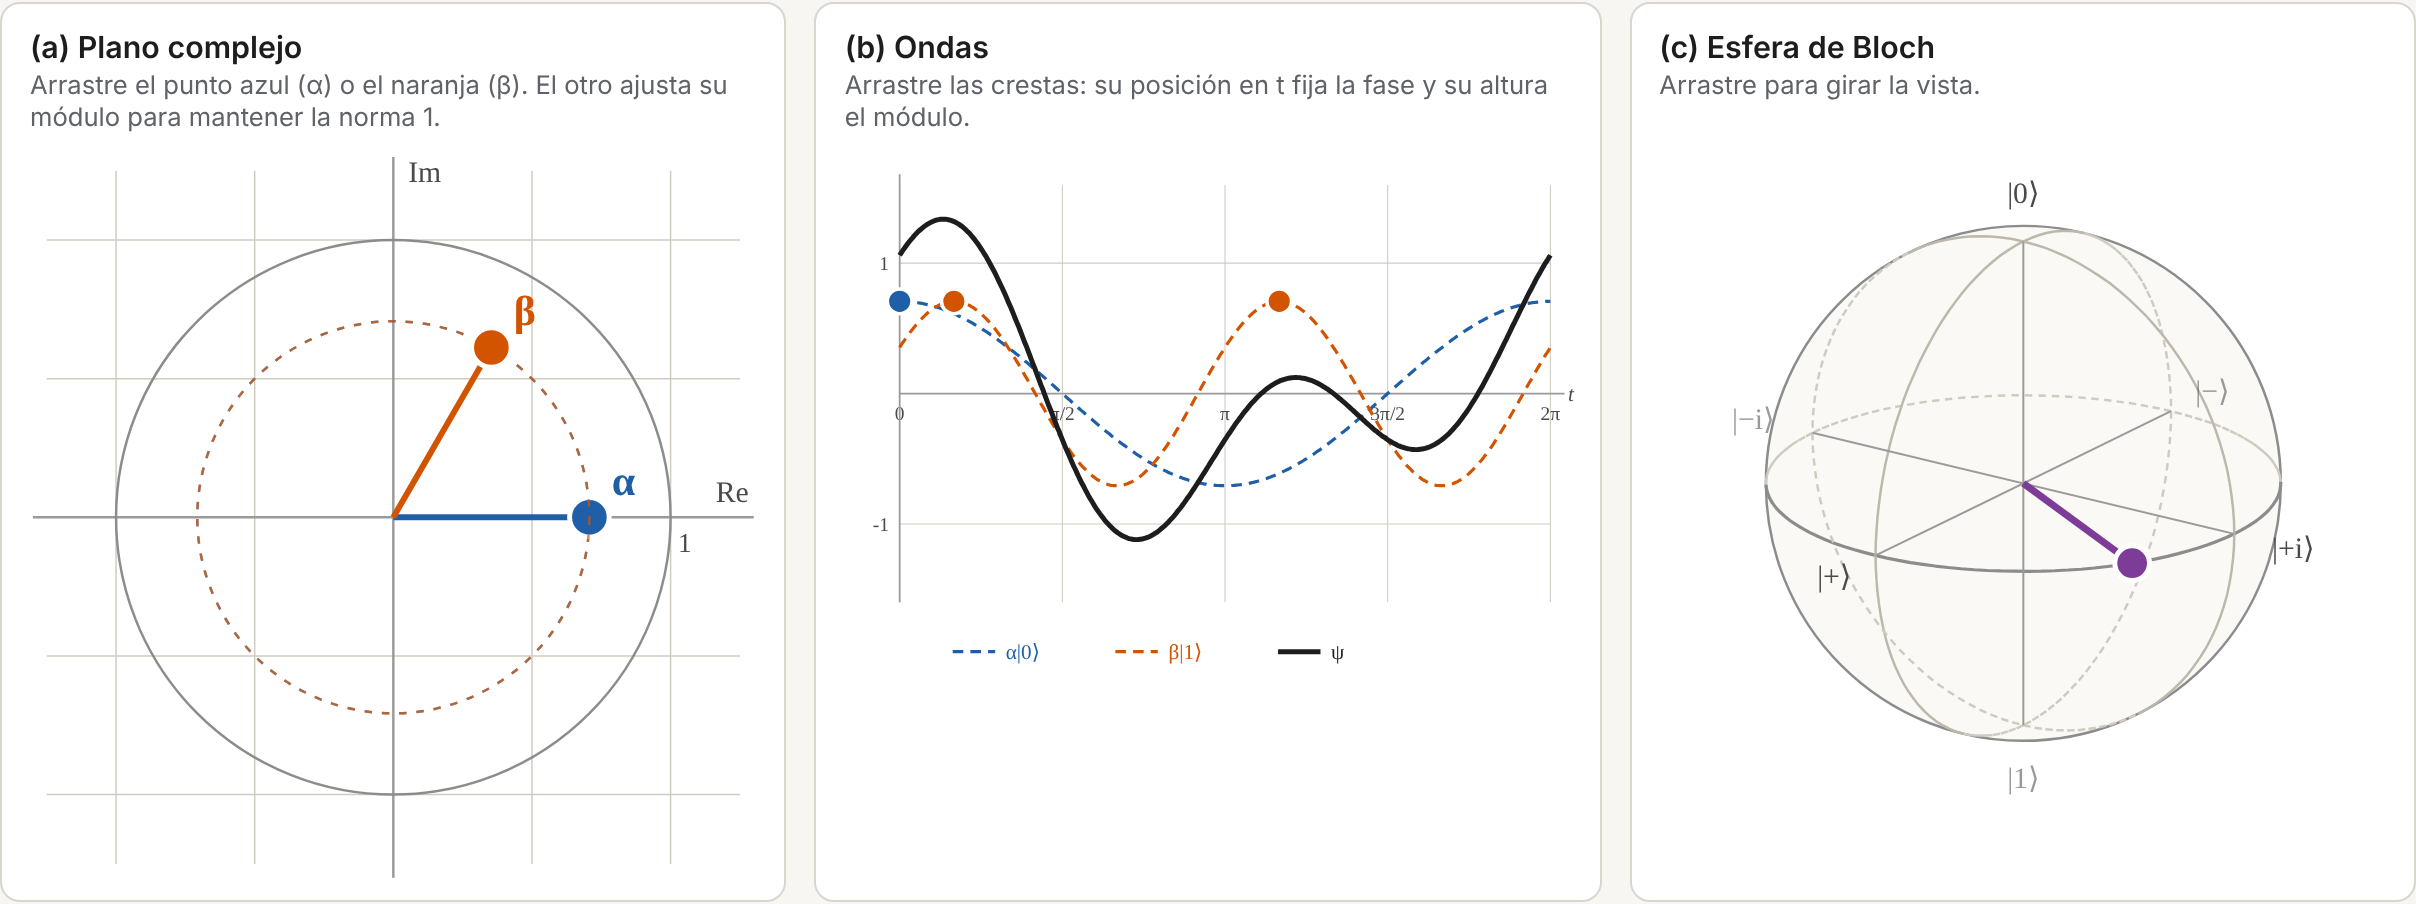
\includegraphics[width=\linewidth]{Imágenes/widget_punto_1_2.png}
\caption{Los tres paneles del widget para $\alpha=\frac1{\sqrt2}$,
$\beta=\frac1{\sqrt2}e^{i\pi/3}$. En (a) se arrastran los coeficientes, en (b) las crestas de las
ondas y en (c) se gira la esfera; los tres paneles se actualizan a la vez.}
\label{fig:widget}
\end{figure}

%======================================================================
\subsection*{El estado \texorpdfstring{$\ket\psi$}{psi}}
%======================================================================

El objeto que muestran los tres paneles es un estado de un qubit en el espacio $V$ del
punto~1.1. Allí se vio, en la ecuación~$f=\alpha\cdot\cos t+\beta\cdot\cos 2t$ \eqref{eq:alfa-beta}, que todo elemento de $V$ se escribe
como
\[
  f=\alpha\cdot\cos t+\beta\cdot\cos 2t=\alpha\ket0+\beta\ket1,\qquad \alpha,\beta\in\mathbb C,
\]
y que esta escritura es única: por el lema~\ref{lema:independencia}, las funciones $\cos t$,
$\sin t$, $\cos 2t$ y $\sin 2t$ son linealmente independientes, de modo que dos expresiones que
dan la misma función tienen los mismos coeficientes. También se vio, en la
ecuación~$\bk fg=\overline\alpha\,\alpha'+\overline\beta\,\beta'$ \eqref{eq:hermitico-coord}, que el producto hermítico de
$f=\alpha\ket0+\beta\ket1$ y $g=\alpha'\ket0+\beta'\ket1$ es
\[
  \bk fg=\overline\alpha\,\alpha'+\overline\beta\,\beta' ,
\]
así que la norma al cuadrado de $f$ es $\bk ff=\overline\alpha\alpha+\overline\beta\beta
=|\alpha|^2+|\beta|^2$.

\begin{definicionT}[Estado de un qubit]
Un \emph{estado} de un qubit es un vector de $V$ de norma $1$,
\begin{equation}\label{eq:estado}
  \ket\psi=\alpha\ket0+\beta\ket1,\qquad \alpha,\beta\in\mathbb C,\qquad |\alpha|^2+|\beta|^2=1 .
\end{equation}
Los números $\alpha$ y $\beta$ se llaman \emph{coeficientes} o \emph{amplitudes} del estado. Al
medir el qubit en la base $\{\ket0,\ket1\}$ se obtiene el resultado $0$ con probabilidad
$|\alpha|^2$ y el resultado $1$ con probabilidad $|\beta|^2$ (regla de Born); la condición
$|\alpha|^2+|\beta|^2=1$ dice que estas dos probabilidades suman $1$.
\end{definicionT}

El widget trabaja siempre con estados: cuando se modifica uno de los coeficientes, el otro
ajusta su módulo para que se siga cumpliendo $|\alpha|^2+|\beta|^2=1$.

\paragraph{Los coeficientes en forma polar.}
La regla de multiplicación del enunciado,
\[
  (Ae^{ix})\cdot\cos nt=A\cos(nt-x),
\]
está escrita en términos de la forma polar de un número complejo. Para aplicarla a $\alpha$ y a
$\beta$ es necesario escribirlos de esa manera, y por eso en esta solución se usan las mismas
letras del enunciado.

\begin{definicionT}[Módulos y fases de los coeficientes]
Los coeficientes del estado $\ket\psi=\alpha\ket0+\beta\ket1$ se escriben en forma polar como
\begin{equation}\label{eq:polar-ab}
  \destacado{\alpha=A\,e^{ix},\qquad \beta=B\,e^{iy},\qquad A,B\ge 0,\quad x,y\in\mathbb R .}
\end{equation}
Los números $A=|\alpha|$ y $B=|\beta|$ son los \emph{módulos} de los coeficientes y los ángulos
$x$ y $y$ son sus \emph{fases}. La condición de norma $1$ se escribe $A^2+B^2=1$. Como $e^{ix}$
no cambia al sumar $2\pi$ a $x$, las fases están determinadas salvo múltiplos enteros de $2\pi$;
las igualdades entre fases se entienden en ese sentido y se escriben con el símbolo $\equiv$: para dos ángulos $a$ y $b$, la notación $a\equiv b\pmod{2\pi}$ significa que $a-b$ es un múltiplo entero de $2\pi$, es decir, que $a$ y $b$ representan el mismo ángulo. La abreviatura ``mód'' viene de ``módulo $2\pi$'' y no tiene relación con el módulo $|\alpha|$ de un número complejo. Cuando no hay confusión se escribe solo $a\equiv b$. Si
$A=0$, entonces $\alpha=0$ para cualquier valor de $x$, y la fase $x$ no está determinada (lo
mismo ocurre con $y$ si $B=0$).
\end{definicionT}

En el estado del ejemplo, $\alpha=\frac1{\sqrt2}=\frac1{\sqrt2}e^{i0}$ y
$\beta=\frac1{\sqrt2}e^{i\pi/3}$, de modo que
\[
  A=B=\tfrac1{\sqrt2},\qquad x=0,\qquad y=\tfrac\pi3 .
\]

%======================================================================
\subsection*{Las tres representaciones del estado}
%======================================================================

Los tres paneles no muestran tres objetos distintos sino el mismo estado $\ket\psi$ descrito de
tres maneras. Cada una usa un tipo de objeto matemático diferente.

\paragraph{Panel (a): dos números complejos.}
En el panel (a), el estado se describe por la pareja de coeficientes $(\alpha,\beta)$. Cada
coeficiente es un número complejo y se dibuja como un punto del plano complejo: el módulo ($A$ o
$B$) es la distancia del punto al origen y la fase ($x$ o $y$) es el ángulo que forma el segmento
que lo une con el origen, medido desde el eje real (figura~\ref{fig:a-b}, izquierda). Como
$A^2+B^2=1$, ambos puntos están dentro del círculo de radio $1$, y si uno se aleja del origen el
otro tiene que acercarse.

\paragraph{Panel (b): una función, es decir, una onda.}
En el panel (b), el estado se describe por lo que es como elemento de $V$: una función
$\psi\colon[0,2\pi]\to\mathbb R$. Según la sección siguiente, esa función es la suma de dos
ondas, una de frecuencia $1$, que proviene de $\alpha\ket0$, y otra de frecuencia $2$, que
proviene de $\beta\ket1$ (figura~\ref{fig:a-b}, derecha). En este contexto, \emph{onda} significa
una función de la forma $A\cos(nt-x)$: una curva que oscila entre $-A$ y $A$ y que completa $n$
oscilaciones en $[0,2\pi]$.

\paragraph{Panel (c): un punto de una esfera.}
En el panel (c), el estado se describe por un punto $\vec r=(r_x,r_y,r_z)\in\mathbb R^3$ de la
esfera de radio $1$ centrada en el origen, llamada esfera de Bloch. Este punto no guarda toda la
información del estado, sino solo la que tiene significado físico; la parte que descarta es la
fase global, que se define más adelante.

\medskip
La tabla siguiente resume las tres descripciones y cuántos números reales usa cada una.
\[
\renewcommand{\arraystretch}{1.35}
\begin{array}{l|l|l}
\text{Panel} & \text{Objeto} & \text{Números reales que lo determinan}\\ \hline
\text{(a) coeficientes} & (\alpha,\beta)\in\mathbb C^2 & A,\ x,\ B,\ y\ \ (\text{con } A^2+B^2=1)\\
\text{(b) onda} & \psi(t)=A\cos(t-x)+B\cos(2t-y) & \text{los mismos } A,\ x,\ B,\ y\\
\text{(c) esfera} & \vec r\in\mathbb R^3,\ \lVert\vec r\rVert=1 & \text{dos ángulos } \theta,\ \varphi
\end{array}
\]
Las descripciones (a) y (b) contienen exactamente la misma información, porque cada pareja
$(\alpha,\beta)$ corresponde a una única función de $V$ y viceversa (por la unicidad de los
coeficientes recordada al comienzo); pasar de una a la otra es una traducción que no pierde
nada. En cambio, la descripción (c) usa un número menos: al pasar a la esfera se pierde la fase
global, y al volver de la esfera hay que elegirla. La figura~\ref{fig:mapa} resume las seis
traducciones, y al final de la solución se reúnen todas sus fórmulas.

\begin{figure}[htbp]
\centering
\begin{tikzpicture}[
  caja/.style={draw=#1, very thick, rounded corners=2mm, fill=#1!6,
               align=center, minimum width=4.4cm, minimum height=1.45cm, font=\small},
  flecha/.style={-{Stealth[length=2.5mm]}, thick, black!70},
  etq/.style={font=\footnotesize, align=center, fill=white, inner sep=1.5pt}
]
  \node[caja=colCu] (a) at (0,0)    {\textbf{(a) Coeficientes}\\[1pt]
        $\alpha=Ae^{ix},\ \beta=Be^{iy}$};
  \node[caja=colSu] (b) at (8.2,0)  {\textbf{(b) Onda}\\[1pt]
        $\psi(t)=A\cos(t-x)+B\cos(2t-y)$};
  \node[caja=colSd] (c) at (4.1,-4) {\textbf{(c) Esfera de Bloch}\\[1pt]
        $\vec r=(\sin\theta\cos\varphi,\,\sin\theta\sin\varphi,\,\cos\theta)$};
  % (a) <-> (b)
  \draw[flecha] ([yshift=3mm]a.east) -- node[etq, above=1pt]{regla del enunciado \eqref{eq:a-b}}
        ([yshift=3mm]b.west);
  \draw[flecha] ([yshift=-3mm]b.west) -- node[etq, below=1pt]{lectura de las crestas \eqref{eq:b-a}} ([yshift=-3mm]a.east);
  % (a) <-> (c)
  \draw[flecha] ([xshift=-8mm]a.south) -- ([xshift=-14mm]c.north);
  \draw[flecha] ([xshift=-6mm]c.north) -- ([xshift=0mm]a.south);
  \node[etq, anchor=east] at (0.15,-2.05) {$\downarrow$ se olvida la fase global \eqref{eq:theta}, \eqref{eq:phi}\\
        $\uparrow$ se elige la fase global $\gamma$ \eqref{eq:c-a}};
  % (b) <-> (c)
  \draw[flecha] ([xshift=0mm]b.south) -- ([xshift=6mm]c.north);
  \draw[flecha] ([xshift=14mm]c.north) -- ([xshift=8mm]b.south);
  \node[etq, anchor=west] at (8.0,-2.05) {$\downarrow$ se olvida la fase global \eqref{eq:b-c}\\
        $\uparrow$ se elige la fase global $\gamma$ \eqref{eq:c-b}};
\end{tikzpicture}
\caption{Las tres representaciones del estado $\ket\psi$ y las fórmulas que traducen entre
ellas. Entre (a) y (b) la traducción no pierde información; hacia (c) se pierde la fase global
$\gamma$, y desde (c) hay que elegirla.}
\label{fig:mapa}
\end{figure}

%======================================================================
\subsection*{De los coeficientes a la onda: del panel (a) al panel (b)}
%======================================================================

\paragraph{Qué se traduce.}
Se parte de dos números complejos, $\alpha$ y $\beta$, y se quiere obtener la función
$\psi(t)$ que representan. No se trata solo de cambiar la escritura de $\alpha$ y $\beta$ a forma
polar: la forma polar es la herramienta que permite aplicar la regla del enunciado, y el
resultado de aplicarla es una función de $t$, no otro número.

\paragraph{Fórmula.}
El estado es la suma de $\alpha\ket0=\alpha\cdot\cos t$ y $\beta\ket1=\beta\cdot\cos 2t$. Al
aplicar la regla del enunciado, $(Ae^{ix})\cdot\cos nt=A\cos(nt-x)$, con $\alpha=Ae^{ix}$ y
$n=1$, y luego con $\beta=Be^{iy}$ y $n=2$, se obtienen las dos ondas que componen el estado; al
sumarlas se obtiene la función completa:
\begin{equation}\label{eq:a-b}
  \destacado{\alpha\ket0=A\cos(t-x),\qquad \beta\ket1=B\cos(2t-y),\qquad
  \psi(t)=A\cos(t-x)+B\cos(2t-y).}
\end{equation}
Si se prefiere la forma rectangular $\alpha=a_1+ib_1$, $\beta=a_2+ib_2$, la
fórmula~$(a+ib)\cdot\cos nt=a\cos nt+b\sin nt$ \eqref{eq:regla-coef} del punto~1.1, $(a+ib)\cdot\cos nt=a\cos nt+b\sin nt$, da la
misma función escrita como $\psi(t)=a_1\cos t+b_1\sin t+a_2\cos 2t+b_2\sin 2t$. La forma polar
tiene la ventaja de que cada número se lee directamente en la gráfica.

\paragraph{Qué significa.}
El módulo de cada coeficiente es la altura de su onda y la fase es cuánto se corre la onda hacia
la derecha. Para ubicar ese corrimiento en la gráfica se sigue la posición de las crestas.

\begin{definicionT}[Cresta]
Una \emph{cresta} de una onda $A\cos(nt-x)$ con $A>0$ es un punto donde la onda alcanza su valor
máximo, $A$. Como $\cos u=1$ exactamente cuando $u$ es un múltiplo entero de $2\pi$, las crestas
son los valores de $t$ con $nt-x=2\pi k$, $k\in\mathbb Z$, es decir, $t=\frac xn+\frac{2\pi k}n$.
\end{definicionT}

La onda $\alpha\ket0=A\cos(t-x)$, de frecuencia $1$, tiene una sola cresta en $[0,2\pi)$, en
$t_\alpha\equiv x$, con altura $A$. La onda $\beta\ket1=B\cos(2t-y)$, de frecuencia $2$, tiene
dos, separadas por $\pi$: la primera en $t_\beta\equiv\frac y2$ y la segunda en $t_\beta+\pi$,
ambas con altura $B$. La fase $y$ se divide entre $2$ porque esa onda oscila el doble de rápido:
un ángulo $y$ corresponde a un corrimiento de solo $y/2$ unidades en $t$. En el ejemplo,
$t_\alpha=0$ y $t_\beta=\frac\pi6$ (figura~\ref{fig:a-b}).

\begin{figure}[htbp]
\centering
\begin{tikzpicture}[scale=1.25, line cap=round]
  \draw[black!15] (-1.25,-1.25) grid[step=0.5] (1.25,1.25);
  \draw[-{Stealth[length=2mm]}, black!60] (-1.35,0) -- (1.45,0) node[right, font=\footnotesize]{Re};
  \draw[-{Stealth[length=2mm]}, black!60] (0,-1.35) -- (0,1.45) node[above, font=\footnotesize]{Im};
  \draw[black!55] (0,0) circle (1);
  \node[font=\scriptsize, black!60, anchor=north west] at (1,0) {$1$};
  % beta = (1/sqrt2) e^{i pi/3}
  \draw[very thick, colSu] (0,0) -- (0.3536,0.6124);
  \fill[colSu] (0.3536,0.6124) circle (0.055);
  \node[colSu, anchor=south west, font=\small] at (0.36,0.6) {$\beta$};
  \draw[thick, colSu] (0.32,0) arc[start angle=0, end angle=60, radius=0.32];
  \node[colSu, font=\scriptsize] at (0.52,0.24) {$y$};
  \node[colSu, font=\scriptsize, rotate=60] at (0.06,0.42) {$B$};
  % alpha = 1/sqrt2
  \draw[very thick, colCu] (0,0) -- (0.7071,0);
  \fill[colCu] (0.7071,0) circle (0.055);
  \node[colCu, anchor=north, font=\small] at (0.7071,-0.05) {$\alpha$};
  \node[colCu, font=\scriptsize, anchor=north] at (0.33,-0.02) {$A$};
\end{tikzpicture}
\hfill
\begin{tikzpicture}
\begin{axis}[ondaT, width=9cm, height=5.4cm, ymin=-1.55, ymax=1.95,
  title={Ondas del estado del ejemplo}]
  \addplot[thick, colCu, densely dashed] {0.7071*cos(x)};
  \addplot[thick, colSu, densely dashed] {0.7071*cos(2*x-pi/3)};
  \addplot[very thick, black!85] {0.7071*cos(x)+0.7071*cos(2*x-pi/3)};
  \fill[colCu] (axis cs:0,0.7071) circle (2.2pt);
  \fill[colSu] (axis cs:pi/6,0.7071) circle (2.2pt);
  \fill[colSu] (axis cs:pi/6+pi,0.7071) circle (2.2pt);
  \draw[colSu, densely dotted] (axis cs:pi/6,0.7071) -- (axis cs:pi/6,0);
  \draw[colSu, densely dotted] (axis cs:pi/6+pi,0.7071) -- (axis cs:pi/6+pi,0);
  \node[colCu, font=\scriptsize, anchor=east] at (axis cs:-0.08,0.62) {$t_\alpha=x=0$};
  \draw[colSu, thin] (axis cs:pi/6,0.7071) -- (axis cs:0.75,1.5);
  \node[colSu, font=\scriptsize, anchor=south west] at (axis cs:0.7,1.48) {$t_\beta=\frac y2=\frac\pi6$};
  \node[colSu, font=\scriptsize, anchor=south] at (axis cs:pi/6+pi,0.78) {$t_\beta+\pi$};
  \draw[thick, colCu, densely dashed] (axis cs:0.2,-1.3) -- (axis cs:0.65,-1.3);
  \node[font=\scriptsize, anchor=west] at (axis cs:0.67,-1.3) {$\alpha\ket0$};
  \draw[thick, colSu, densely dashed] (axis cs:2.05,-1.3) -- (axis cs:2.5,-1.3);
  \node[font=\scriptsize, anchor=west] at (axis cs:2.52,-1.3) {$\beta\ket1$};
  \draw[very thick, black!85] (axis cs:3.9,-1.3) -- (axis cs:4.35,-1.3);
  \node[font=\scriptsize, anchor=west] at (axis cs:4.37,-1.3) {$\psi(t)$};
\end{axis}
\end{tikzpicture}
\caption{El estado del ejemplo en los paneles (a) y (b). A la izquierda, los coeficientes como
puntos del plano complejo: $\alpha$ (azul) a distancia $A=\frac1{\sqrt2}$ del origen y con fase
$x=0$; $\beta$ (naranja) a distancia $B=\frac1{\sqrt2}$ y con fase $y=\frac\pi3$. A la derecha,
las ondas correspondientes: la altura de cada una es el módulo de su coeficiente y la posición de
sus crestas (puntos) está fijada por la fase. La curva negra es la suma $\psi(t)$.}
\label{fig:a-b}
\end{figure}

%======================================================================
\subsection*{De la onda a los coeficientes: del panel (b) al panel (a)}
%======================================================================

\paragraph{Qué se traduce.}
Se parte de las dos ondas $\alpha\ket0$ y $\beta\ket1$, tal como aparecen en el panel (b), y se
quieren recuperar los dos números complejos que las producen. Es la traducción inversa de la
anterior.

\paragraph{Fórmula.}
Por la ecuación~$\alpha\ket0=A\cos(t-x),\quad\penalty0 \beta\ket1=B\cos(2t-y),\quad\penalty0 \psi(t)=A\cos(t-x)+B\cos(2t-y)$ \eqref{eq:a-b}, $\alpha\ket0=A\cos(t-x)$ tiene altura $A$ y cresta en
$t_\alpha\equiv x$, y $\beta\ket1=B\cos(2t-y)$ tiene altura $B$ y primera cresta en
$t_\beta\equiv\frac y2$. Al despejar los cuatro números se obtiene
\begin{equation}\label{eq:b-a}
  \destacado{A=\text{altura de }\alpha\ket0,\quad x\equiv t_\alpha,\qquad
  B=\text{altura de }\beta\ket1,\quad y\equiv 2t_\beta ,}
\end{equation}
y con ellos $\alpha=Ae^{ix}$ y $\beta=Be^{iy}$. El factor $2$ en la última igualdad deshace la
división entre $2$ de la sección anterior.

\paragraph{Qué significa.}
Leer una onda es leer un número complejo: la altura da el módulo y la posición de la cresta da
la fase. En el ejemplo de la figura~\ref{fig:a-b}, ambas alturas son $\frac1{\sqrt2}$, la cresta
azul está en $t_\alpha=0$ y la primera cresta naranja en $t_\beta=\frac\pi6$, de donde $x=0$,
$y=2\cdot\frac\pi6=\frac\pi3$, y se recuperan $\alpha=\frac1{\sqrt2}$ y
$\beta=\frac1{\sqrt2}e^{i\pi/3}$.

%======================================================================
\subsection*{Fase global y fase relativa}
%======================================================================

Antes de las traducciones que involucran el panel (c) hace falta precisar qué parte del estado
se descarta al pasar a la esfera. Para eso se usa una propiedad de la multiplicación de números
complejos en forma polar: al multiplicar dos números se multiplican los módulos y se suman las
fases,
\[
  \bigl(r_1e^{i\omega_1}\bigr)\bigl(r_2e^{i\omega_2}\bigr)=r_1r_2\,e^{i(\omega_1+\omega_2)} .
\]
En particular, multiplicar un número complejo por $e^{i\gamma}$, que tiene módulo $1$, no cambia
su módulo y le suma $\gamma$ a su fase; en el plano complejo, el punto gira un ángulo $\gamma$
alrededor del origen.

\begin{definicionT}[Fase global]
Dos estados $\ket\psi$ y $\ket{\psi'}$ \emph{difieren en una fase global} si existe
$\gamma\in\mathbb R$ tal que $\ket{\psi'}=e^{i\gamma}\ket\psi$, es decir, si los dos coeficientes
se multiplican por el mismo número $e^{i\gamma}$:
\[
  \alpha'=e^{i\gamma}\alpha=Ae^{i(x+\gamma)},\qquad \beta'=e^{i\gamma}\beta=Be^{i(y+\gamma)} .
\]
En computación cuántica, dos estados que difieren en una fase global describen la misma
situación física, y por eso se identifican; se escribe $\ket{\psi'}\sim\ket\psi$.
\end{definicionT}

En el panel (a), una fase global hace girar los dos puntos $\alpha$ y $\beta$ el mismo ángulo
$\gamma$ alrededor del origen, como si estuvieran pegados (figura~\ref{fig:fases}, izquierda).
Los módulos $A$ y $B$ no cambian, así que tampoco cambian las probabilidades $A^2$ y $B^2$ de
obtener $0$ o $1$ al medir.

La razón para identificar los dos estados es que ninguna medición los distingue, no solo la
medición en la base $\{\ket0,\ket1\}$. Al medir en cualquier base ortonormal, las probabilidades
son de la forma $|\bk\phi\psi|^2$ para algún estado $\ket\phi$ de esa base (regla de Born). Por
la linealidad del producto hermítico en el segundo argumento, propiedad (H2) del punto~1.1,
$\bk\phi{e^{i\gamma}\psi}=e^{i\gamma}\bk\phi\psi$, y como $|e^{i\gamma}|=1$,
\[
  \bigl|\bk\phi{e^{i\gamma}\psi}\bigr|^2=|e^{i\gamma}|^2\,|\bk\phi\psi|^2=|\bk\phi\psi|^2 .
\]
Todas las probabilidades coinciden, de modo que no hay experimento que separe $\ket\psi$ de
$e^{i\gamma}\ket\psi$.

Lo que sí se conserva al girar los dos puntos juntos es el ángulo entre ellos, medido desde el
origen. Antes del giro es $y-x$, y después es $(y+\gamma)-(x+\gamma)=y-x$.

\begin{definicionT}[Fase relativa]
La \emph{fase relativa} del estado $\ket\psi=Ae^{ix}\ket0+Be^{iy}\ket1$ es la diferencia
$y-x$ entre las fases de sus dos coeficientes. En el plano complejo, es el ángulo que hay que
girar desde el punto $\alpha$ hasta el punto $\beta$.
\end{definicionT}

A diferencia de la fase global, la fase relativa sí cambia el estado. Por ejemplo, los estados
\[
  \ket+=\tfrac1{\sqrt2}\ket0+\tfrac1{\sqrt2}\ket1,\qquad
  \ket-=\tfrac1{\sqrt2}\ket0-\tfrac1{\sqrt2}\ket1=\tfrac1{\sqrt2}\ket0+\tfrac1{\sqrt2}e^{i\pi}\ket1
\]
tienen los mismos módulos, $A=B=\frac1{\sqrt2}$, y por tanto las mismas probabilidades al medir
en la base $\{\ket0,\ket1\}$, pero fases relativas $0$ y $\pi$ (figura~\ref{fig:fases},
derecha). No difieren en una fase global, pues para pasar del uno al otro hay que multiplicar
solo $\beta$ por $-1$. Su producto hermítico, con la fórmula
$\bk fg=\overline\alpha\,\alpha'+\overline\beta\,\beta'$, es
\[
  \bk+-=\tfrac1{\sqrt2}\cdot\tfrac1{\sqrt2}+\tfrac1{\sqrt2}\cdot\bigl(-\tfrac1{\sqrt2}\bigr)
  =\tfrac12-\tfrac12=0 ,
\]
así que son ortogonales; una medición en la base $\{\ket+,\ket-\}$ los distingue con certeza.

\begin{figure}[htbp]
\centering
\begin{tikzpicture}[scale=1.55, line cap=round]
  \draw[black!12] (-1.2,-1.2) grid[step=0.5] (1.2,1.2);
  \draw[-{Stealth[length=2mm]}, black!60] (-1.3,0) -- (1.4,0) node[right, font=\footnotesize]{Re};
  \draw[-{Stealth[length=2mm]}, black!60] (0,-1.3) -- (0,1.4) node[above, font=\footnotesize]{Im};
  \draw[black!45] (0,0) circle (1);
  % estado original: alpha = (1/sqrt2) e^{i0}, beta = (1/sqrt2) e^{i pi/3}
  \draw[thick, colCu] (0,0) -- (0.7071,0);
  \fill[colCu] (0.7071,0) circle (0.045);
  \node[colCu, font=\scriptsize, anchor=north] at (0.72,-0.03) {$\alpha$};
  \draw[thick, colSu] (0,0) -- (0.3536,0.6124);
  \fill[colSu] (0.3536,0.6124) circle (0.045);
  \node[colSu, font=\scriptsize, anchor=west] at (0.38,0.64) {$\beta$};
  \draw[resaltado, thick] (0.3,0) arc[start angle=0, end angle=60, radius=0.3];
  \node[resaltado, font=\scriptsize] at (0.47,0.17) {$\frac\pi3$};
  % girado gamma = pi/2: alpha' = (1/sqrt2) e^{i pi/2}, beta' = (1/sqrt2) e^{i 5pi/6}
  \draw[thick, colCu, densely dashed] (0,0) -- (0,0.7071);
  \fill[colCu] (0,0.7071) circle (0.045);
  \node[colCu, font=\scriptsize, anchor=east] at (-0.03,0.74) {$\alpha'$};
  \draw[thick, colSu, densely dashed] (0,0) -- (-0.6124,0.3536);
  \fill[colSu] (-0.6124,0.3536) circle (0.045);
  \node[colSu, font=\scriptsize, anchor=east] at (-0.63,0.36) {$\beta'$};
  \draw[resaltado, thick] (0,0.3) arc[start angle=90, end angle=150, radius=0.3];
  \node[resaltado, font=\scriptsize] at (-0.2,0.47) {$\frac\pi3$};
  % flecha del giro
  \draw[-{Stealth[length=1.6mm]}, black!55] (1.1,0.0) arc[start angle=0, end angle=85, radius=1.1];
  \node[black!65, font=\scriptsize, anchor=south west] at (0.8,0.8) {$\gamma=\frac\pi2$};
  \node[font=\small] at (0,-1.55) {Fase global: mismo estado};
\end{tikzpicture}
\hspace{1.2cm}
\begin{tikzpicture}[scale=1.55, line cap=round]
  \draw[black!12] (-1.2,-1.2) grid[step=0.5] (1.2,1.2);
  \draw[-{Stealth[length=2mm]}, black!60] (-1.3,0) -- (1.4,0) node[right, font=\footnotesize]{Re};
  \draw[-{Stealth[length=2mm]}, black!60] (0,-1.3) -- (0,1.4) node[above, font=\footnotesize]{Im};
  \draw[black!45] (0,0) circle (1);
  % |+>: alpha = beta = 1/sqrt2 ; |->: alpha = 1/sqrt2, beta = -1/sqrt2
  \draw[thick, colCu] (0,0) -- (0.7071,0);
  \fill[colCu] (0.7071,0) circle (0.045);
  \fill[colSu] (0.7071,0) circle (0.028);
  \node[font=\scriptsize, anchor=north] at (0.72,-0.06) {$\alpha=\beta$ en $\ket+$};
  \draw[thick, colSu, densely dashed] (0,0) -- (-0.7071,0);
  \fill[colSu] (-0.7071,0) circle (0.045);
  \node[colSu, font=\scriptsize, anchor=north] at (-0.72,-0.06) {$\beta$ en $\ket-$};
  \draw[resaltado, thick, -{Stealth[length=1.6mm]}] (0.35,0) arc[start angle=0, end angle=180, radius=0.35];
  \node[resaltado, font=\scriptsize] at (0,0.5) {$\pi$};
  \node[font=\small] at (0,-1.55) {Fase relativa: cambia el estado};
\end{tikzpicture}
\caption{Izquierda: al multiplicar el estado del ejemplo por $e^{i\pi/2}$, los puntos $\alpha$ y
$\beta$ (continuos) giran juntos un ángulo $\pi/2$ hasta $\alpha'$ y $\beta'$ (punteados). Los
módulos y el ángulo $\frac\pi3$ entre los dos puntos no cambian, y el estado se identifica con el
original. Derecha: $\ket+$ y $\ket-$ tienen los mismos módulos, pero en $\ket-$ solo $\beta$ gira
un ángulo $\pi$; la fase relativa pasa de $0$ a $\pi$ y el estado es otro.}
\label{fig:fases}
\end{figure}

En resumen, de los cuatro números $A$, $x$, $B$, $y$ que describen el estado en el panel (a),
la fase global hace que uno sobre: salvo fase global, el estado queda determinado por cómo se
reparte la probabilidad entre $\ket0$ y $\ket1$ (los módulos $A$ y $B$, ligados por
$A^2+B^2=1$) y por la fase relativa $y-x$. Son dos datos, y la esfera de Bloch representa
exactamente esos dos datos.

\begin{definicionT}[Ángulos de la esfera de Bloch]
Todo punto de la esfera de radio $1$ centrada en el origen se describe con dos ángulos: la
\emph{inclinación} $\theta\in[0,\pi]$, que es el ángulo entre el punto y el polo norte (el eje
$z$), y la \emph{longitud} $\varphi$, que es el ángulo medido sobre el ecuador desde el eje $x$,
como la longitud en un mapa. Sus coordenadas son
\[
  \vec r=(\sin\theta\cos\varphi,\ \sin\theta\sin\varphi,\ \cos\theta).
\]
Con $\theta=0$ el punto está en el polo norte, con $\theta=\frac\pi2$ en el ecuador y con
$\theta=\pi$ en el polo sur. La \emph{esfera de Bloch} es esta esfera cuando cada punto se
interpreta como un estado de un qubit: el polo norte corresponde a $\ket0$ y el polo sur a
$\ket1$ (figura~\ref{fig:bloch}).
\end{definicionT}

\begin{figure}[htbp]
\centering
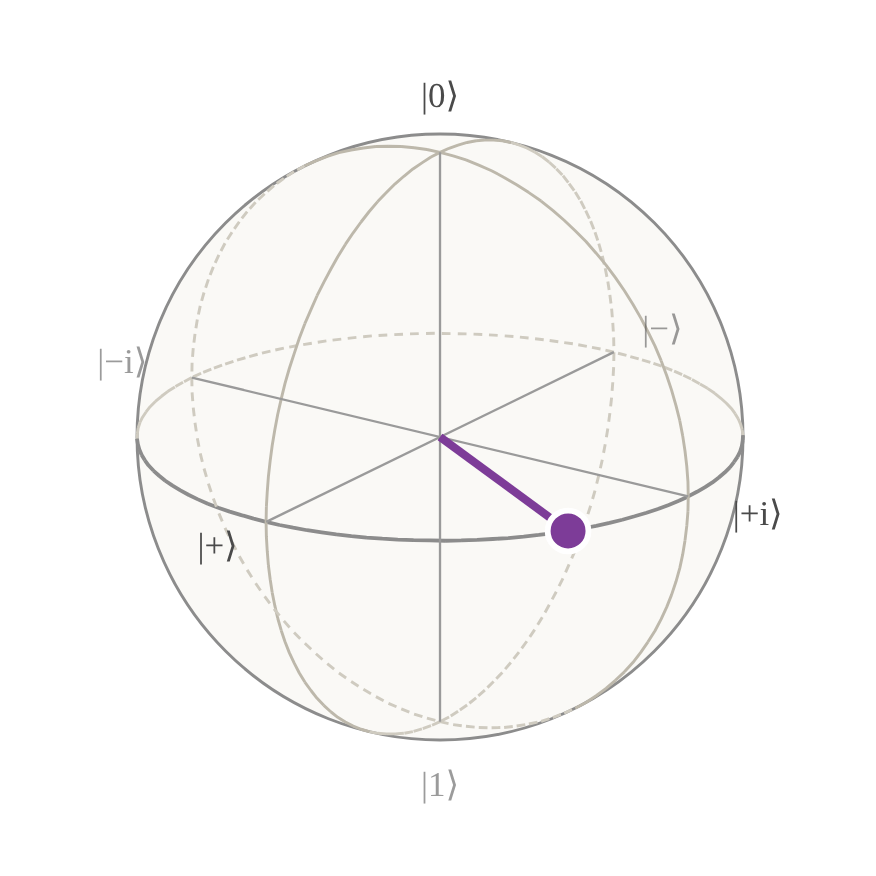
\includegraphics[width=0.66\linewidth]{Imágenes/p12_bloch_ejemplo.png}
\caption{Esfera de Bloch del widget (panel (c)) para el estado del ejemplo, $\alpha=\frac1{\sqrt2}$, $\beta=\frac1{\sqrt2}e^{i\pi/3}$. Su inclinación es $\theta=\frac\pi2$ (está en el ecuador) y su longitud es $\varphi=\frac\pi3$. Los polos son $\ket0$ y $\ket1$, y sobre los ejes del ecuador están $\ket+$ y $\ket{{+}i}$ (con sus opuestos $\ket-$ y $\ket{{-}i}$).}
\label{fig:bloch}
\end{figure}

%======================================================================
\subsection*{De los coeficientes a la esfera: del panel (a) al panel (c)}
%======================================================================

\paragraph{Qué se traduce.}
Se parte de los cuatro números del panel (a), $\alpha=Ae^{ix}$ y $\beta=Be^{iy}$, y se quiere un
punto de la esfera, es decir, dos ángulos: la inclinación $\theta$ y la longitud $\varphi$. Como
la esfera solo guarda los dos datos que no dependen de la fase global, la traducción consiste en
deshacerse de la fase global y escribir los dos datos que quedan como ángulos: el reparto entre
$A$ y $B$ se convierte en $\theta$ y la fase relativa en $\varphi$.

\paragraph{Se quita la fase global.}
Como $e^{ix}e^{-ix}=1$, el coeficiente $\beta$ se puede escribir como
$Be^{iy}=e^{ix}\,Be^{i(y-x)}$, y el factor $e^{ix}$ sale de los dos términos:
\[
  \ket\psi=Ae^{ix}\ket0+Be^{iy}\ket1
  =e^{ix}\bigl(A\ket0+Be^{i(y-x)}\ket1\bigr).
\]
El factor $e^{ix}$ es una fase global, así que $\ket\psi$ se identifica con el estado entre
paréntesis, $A\ket0+Be^{i(y-x)}\ket1$. En ese estado el primer coeficiente es el número real
$A\ge0$, y la única fase que queda es la fase relativa, que se toma como longitud:
\begin{equation}\label{eq:phi}
  \destacado{\varphi\equiv y-x \pmod{2\pi}.}
\end{equation}

\paragraph{El reparto entre $A$ y $B$ se convierte en un ángulo.}
Quedan dos números, $A$ y $B$, pero no son independientes: si se conoce $A$, la condición
$A^2+B^2=1$ y $B\ge0$ dan $B=\sqrt{1-A^2}$. Una manera de describir la pareja con un solo número
es verla como un punto $(A,B)$ del plano. Ese punto está a distancia $\sqrt{A^2+B^2}=1$ del
origen, y como $A,B\ge0$, está en el primer cuadrante, es decir, sobre el cuarto de
circunferencia de la figura~\ref{fig:theta}. Un punto de ese cuarto de circunferencia queda
determinado por el ángulo $\omega\in[0,\frac\pi2]$ que forma con el eje horizontal, y sus
coordenadas son $A=\cos\omega$ y $B=\sin\omega$ (son las coordenadas polares de un punto a
distancia $1$ del origen).

El ángulo $\omega$ mide cómo se reparte la probabilidad: con $\omega=0$ se tiene $A=1$, $B=0$ y
el resultado es $0$ con certeza; con $\omega=\frac\pi2$ se tiene $A=0$, $B=1$ y el resultado es
$1$ con certeza; con $\omega=\frac\pi4$, $A=B=\frac1{\sqrt2}$ y los dos resultados tienen
probabilidad $\frac12$.

Falta ubicar ese reparto en la esfera. La esfera de Bloch pone $\ket0$ en el polo norte, donde
$\theta=0$, y $\ket1$ en el polo sur, donde $\theta=\pi$; se eligen puntos opuestos porque
$\ket0$ y $\ket1$ son ortogonales, $\bk01=0$. Así, cuando $\omega$ va de $0$ a $\frac\pi2$, la
inclinación tiene que ir de $0$ a $\pi$, que es el doble. Por eso se toma $\theta=2\omega$, o
sea, $\omega=\frac\theta2$, y las igualdades $A=\cos\omega$, $B=\sin\omega$ se convierten en
\begin{equation}\label{eq:theta}
  \destacado{\cos\tfrac\theta2=A,\qquad \sin\tfrac\theta2=B .}
\end{equation}
El $\frac12$ en $\frac\theta2$ no es una convención arbitraria: es lo que hace que el cuarto de
circunferencia, que solo abarca un ángulo de $\frac\pi2$, cubra en la esfera todo el camino de
un polo al otro.

\begin{figure}[htbp]
\centering
\begin{tikzpicture}[scale=2.6, line cap=round]
  \draw[-{Stealth[length=2mm]}, black!60] (-0.08,0) -- (1.25,0) node[right, font=\footnotesize]{$A$};
  \draw[-{Stealth[length=2mm]}, black!60] (0,-0.08) -- (0,1.25) node[above, font=\footnotesize]{$B$};
  \draw[very thick, colSd] (1,0) arc[start angle=0, end angle=90, radius=1];
  \draw[thick, black!80] (0,0) -- (0.866,0.5);
  \draw[densely dotted, black!60] (0.866,0.5) -- (0.866,0);
  \draw[densely dotted, black!60] (0.866,0.5) -- (0,0.5);
  \fill[black!85] (0.866,0.5) circle (0.022);
  \node[font=\scriptsize, anchor=south west] at (0.87,0.5) {$(A,B)$};
  \draw[resaltado, thick] (0.28,0) arc[start angle=0, end angle=30, radius=0.28];
  \node[resaltado, font=\scriptsize, anchor=west] at (0.30,0.055) {$\omega=\frac\theta2$};
  \node[font=\scriptsize, anchor=north] at (0.866,0) {$\cos\frac\theta2$};
  \node[font=\scriptsize, anchor=east] at (0,0.5) {$\sin\frac\theta2$};
  \fill[colCu] (1,0) circle (0.025);
  \node[colCu, font=\scriptsize, anchor=north west] at (1,0) {$\ket0$: $A=1$};
  \fill[colSu] (0,1) circle (0.025);
  \node[colSu, font=\scriptsize, anchor=south west] at (0.02,1.0) {$\ket1$: $B=1$};
  \node[font=\scriptsize, anchor=north] at (0.5,-0.2) {$\omega$ va de $0$ a $\frac\pi2$};
\end{tikzpicture}

\caption{El punto $(A,B)$ está sobre un cuarto de circunferencia y queda determinado por el ángulo $\omega$. De $\ket0$ a $\ket1$, el ángulo $\omega$ recorre solo $\frac\pi2$. En la esfera de Bloch, en cambio, la inclinación $\theta$ va de $\ket0$ (polo norte) a $\ket1$ (polo sur) y recorre $\pi$, el doble. Por eso $\theta=2\omega$, de modo que $A=\cos\frac\theta2$ y $B=\sin\frac\theta2$.}
\label{fig:theta}
\end{figure}

La tabla siguiente muestra los tres casos de referencia.
\[
\renewcommand{\arraystretch}{1.35}
\begin{array}{c|c|c|c|l}
A & B & \omega=\theta/2 & \theta & \text{Posición en la esfera}\\ \hline
1 & 0 & 0 & 0 & \text{polo norte, } \ket0\\
\frac1{\sqrt2} & \frac1{\sqrt2} & \frac\pi4 & \frac\pi2 & \text{ecuador}\\
0 & 1 & \frac\pi2 & \pi & \text{polo sur, } \ket1
\end{array}
\]

\paragraph{Fórmula.}
Al reunir $\varphi\equiv y-x$ y $\cos\frac\theta2=A$, $\sin\frac\theta2=B$, el estado entre
paréntesis se escribe con los dos ángulos, y salvo fase global, todo estado tiene la forma
\begin{equation}\label{eq:forma-bloch}
  \ket\psi\sim\cos\tfrac\theta2\,\ket0+e^{i\varphi}\sin\tfrac\theta2\,\ket1,
  \qquad \theta\in[0,\pi],\ \varphi\in(-\pi,\pi] ,
\end{equation}
que es la forma con la que la esfera de Bloch se presenta en la bibliografía del curso (Nielsen
y Chuang, sección~1.2).

El punto también se puede calcular sin pasar por los ángulos. Con $\cos\frac\theta2=A$,
$\sin\frac\theta2=B$ y $\varphi\equiv y-x$ se tiene
$\overline\alpha\beta=Ae^{-ix}Be^{iy}=AB\,e^{i(y-x)}=\cos\frac\theta2\sin\frac\theta2\,e^{i\varphi}$,
y por las fórmulas del ángulo doble, $2\sin\frac\theta2\cos\frac\theta2=\sin\theta$ y
$\cos^2\frac\theta2-\sin^2\frac\theta2=\cos\theta$. Por tanto,
$2\overline\alpha\beta=\sin\theta\,e^{i\varphi}=\sin\theta\cos\varphi+i\sin\theta\sin\varphi$ y
$A^2-B^2=\cos\theta$. Con la notación del punto 1.1, en la que $\Real z=a$ es la parte real e $\Imag z=b$ la parte imaginaria de $z=a+ib$, se obtiene
\begin{equation}\label{eq:a-c}
  \destacado{\vec r=(\sin\theta\cos\varphi,\ \sin\theta\sin\varphi,\ \cos\theta)
  =\bigl(2\Real(\overline\alpha\beta),\ 2\Imag(\overline\alpha\beta),\ A^2-B^2\bigr).}
\end{equation}
Es decir, se calcula el número complejo $2\overline\alpha\beta$: su parte real es la coordenada $r_x$ del punto y su parte imaginaria es la coordenada $r_y$. En el ejemplo, $2\overline\alpha\beta=2\cdot\frac1{\sqrt2}\cdot\frac1{\sqrt2}e^{i\pi/3}=e^{i\pi/3}=\frac12+i\frac{\sqrt3}{2}$, así que $r_x=\frac12$, $r_y=\frac{\sqrt3}{2}$ y $r_z=\frac12-\frac12=0$.
Esta segunda expresión no usa las fases $x$ y $y$, así que sigue siendo válida cuando $A=0$ o
$B=0$, que es justamente cuando alguna fase no está determinada. En esos casos $\sin\theta=0$ y
el punto está en uno de los polos, de modo que $\varphi$ no hace falta.

\paragraph{Qué significa.}
La altura del punto en la esfera es $r_z=\cos\theta=A^2-B^2$, la diferencia entre la
probabilidad de obtener $0$ y la de obtener $1$. Dicho de otra forma, $r_z$ es el valor esperado de una medición que vale $+1$ si el resultado es $0$ y $-1$ si es $1$: el punto está en
el polo norte cuando el resultado es $0$ con certeza, en el polo sur cuando es $1$ con certeza y
en el ecuador cuando los dos resultados son igualmente probables. La longitud $\varphi$, en
cambio, no se ve en esas probabilidades; es la fase relativa, que no tiene análogo en una moneda clásica con probabilidades $|\alpha|^2$ y $|\beta|^2$. Por ejemplo, $\ket+$ y $\ket-$ están ambos en el ecuador
($\theta=\frac\pi2$), pero en lados opuestos ($\varphi=0$ y $\varphi=\pi$). En el ejemplo,
$A=B=\frac1{\sqrt2}$ da $\cos\theta=\frac12-\frac12=0$, es decir, $\theta=\frac\pi2$ (el
ecuador), y $\varphi=\frac\pi3-0=\frac\pi3$.

%======================================================================
\subsection*{De la esfera a los coeficientes: del panel (c) al panel (a)}
%======================================================================

\paragraph{Qué se traduce.}
Se parte de un punto de la esfera, es decir, de dos ángulos $\theta$ y $\varphi$, y se quieren
dos números complejos. La esfera no guarda la fase global, así que esta traducción no tiene una
única respuesta: a cada punto le corresponde toda una familia de parejas $(\alpha,\beta)$, y
para obtener una hay que elegir la fase global.

\paragraph{Fórmula.}
Por la forma~$\ket\psi\sim\cos\tfrac\theta2\,\ket0+e^{i\varphi}\sin\tfrac\theta2\,\ket1$ \eqref{eq:forma-bloch},
$\ket\psi\sim\cos\frac\theta2\ket0+e^{i\varphi}\sin\frac\theta2\ket1$, el estado
$\cos\frac\theta2\ket0+e^{i\varphi}\sin\frac\theta2\ket1$ corresponde al punto, y todos los demás
difieren de él en una fase global $e^{i\gamma}$. Al multiplicar los dos coeficientes por
$e^{i\gamma}$ se obtiene
\begin{equation}\label{eq:c-a}
  \destacado{\alpha=e^{i\gamma}\cos\tfrac\theta2,\qquad
  \beta=e^{i(\gamma+\varphi)}\sin\tfrac\theta2,\qquad \gamma\in\mathbb R\text{ arbitrario},}
\end{equation}
es decir, $A=\cos\frac\theta2$, $x=\gamma$, $B=\sin\frac\theta2$ y $y=\gamma+\varphi$.

\paragraph{Qué significa.}
Las dos primeras igualdades deshacen las de la traducción anterior: $A=\cos\frac\theta2$ y
$B=\sin\frac\theta2$ recuperan los módulos, y $y-x=(\gamma+\varphi)-\gamma=\varphi$ recupera la
fase relativa. El ángulo $\gamma$ es la fase global elegida. Cambiarlo gira los dos puntos del
panel (a) el mismo ángulo alrededor del origen, como en la figura~\ref{fig:fases}, sin moverlos
del punto de la esfera. En el widget, $\gamma$ se controla con un deslizador que fija
$x=\gamma$.

%======================================================================
\subsection*{De la onda a la esfera: del panel (b) al panel (c)}
%======================================================================

\paragraph{Qué se traduce.}
Se parte de las ondas del panel (b) y se quiere un punto de la esfera. La traducción es la
composición de dos de las anteriores: de las ondas se pasa a los coeficientes leyendo las
crestas, y de los coeficientes a la esfera con $\cos\frac\theta2=A$, $\sin\frac\theta2=B$ y
$\varphi\equiv y-x$.

\paragraph{Fórmula.}
Por la ecuación~$A=\text{altura de }\alpha\ket0,\quad\penalty0 x\equiv t_\alpha,\quad\penalty0 B=\text{altura de }\beta\ket1,\quad\penalty0 y\equiv 2t_\beta$ \eqref{eq:b-a}, $A$ y $B$ son las alturas de las ondas, $x\equiv t_\alpha$ y
$y\equiv 2t_\beta$. Al sustituir estos valores en $\cos\theta=A^2-B^2$ y en
$\varphi\equiv y-x$, los ángulos de la esfera quedan escritos directamente en términos de las
ondas:
\begin{equation}\label{eq:b-c}
  \destacado{\cos\theta=(\text{altura de }\alpha\ket0)^2-(\text{altura de }\beta\ket1)^2,
  \qquad \varphi\equiv 2t_\beta-t_\alpha \pmod{2\pi}.}
\end{equation}

\paragraph{Qué significa.}
La inclinación depende solo de las alturas y la longitud solo de las posiciones de las crestas.
La primera igualdad dice que la altura del punto en la esfera mide cómo se reparte la norma entre
la frecuencia $1$ y la frecuencia $2$: si toda la norma está en $\cos t$, el punto está en el
polo norte, y si toda está en $\cos 2t$, en el polo sur. La segunda dice que la longitud mide el
desfase entre las crestas, pero contado en la escala de la frecuencia $2$; no es la simple
diferencia $t_\beta-t_\alpha$, porque una misma distancia en $t$ corresponde a un ángulo doble en
la onda de frecuencia $2$. En el ejemplo de la figura~\ref{fig:a-b}, ambas alturas son
$\frac1{\sqrt2}$, así que $\cos\theta=0$, y $\varphi=2\cdot\frac\pi6-0=\frac\pi3$, el mismo punto
obtenido desde el panel (a).

%======================================================================
\subsection*{De la esfera a la onda: del panel (c) al panel (b)}
%======================================================================

\paragraph{Qué se traduce.}
Se parte de un punto de la esfera y se quiere una función de $t$. Es la composición de la
traducción de (c) a (a) con la de (a) a (b), y, como la primera, requiere elegir la fase
global.

\paragraph{Fórmula.}
Por la ecuación~$\alpha=e^{i\gamma}\cos\tfrac\theta2,\quad\penalty0 \beta=e^{i(\gamma+\varphi)}\sin\tfrac\theta2$ \eqref{eq:c-a}, $A=\cos\frac\theta2$, $x=\gamma$, $B=\sin\frac\theta2$ y
$y=\gamma+\varphi$. Al sustituir estos valores en la onda de la ecuación~$\alpha\ket0=A\cos(t-x),\quad\penalty0 \beta\ket1=B\cos(2t-y),\quad\penalty0 \psi(t)=A\cos(t-x)+B\cos(2t-y)$ \eqref{eq:a-b},
$\psi(t)=A\cos(t-x)+B\cos(2t-y)$, se obtiene
\begin{equation}\label{eq:c-b}
  \destacado{\psi(t)=\cos\tfrac\theta2\,\cos(t-\gamma)
  +\sin\tfrac\theta2\,\cos(2t-\gamma-\varphi).}
\end{equation}

\paragraph{Qué significa.}
Un mismo punto de la esfera corresponde a toda una familia de ondas, una para cada $\gamma$, y
esas ondas no son simples copias corridas unas de otras, como se explica a continuación.

%======================================================================
\subsection*{Fase global y desplazamientos en el tiempo}
%======================================================================

La onda $\psi(t)=\cos\frac\theta2\cos(t-\gamma)+\sin\frac\theta2\cos(2t-\gamma-\varphi)$ de la
ecuación~$\psi(t)=\cos\tfrac\theta2\,\cos(t-\gamma)+\sin\tfrac\theta2\,\cos(2t-\gamma-\varphi)$ \eqref{eq:c-b} muestra un hecho que el widget permite ver directamente. Al cambiar la
fase global $\gamma$, la onda $\alpha\ket0=\cos\frac\theta2\cos(t-\gamma)$ se corre $\gamma$
hacia la derecha, mientras que
$\beta\ket1=\sin\frac\theta2\cos\bigl(2(t-\frac{\gamma+\varphi}2)\bigr)$ se corre solo
$\gamma/2$. Como las dos componentes se corren distancias distintas, la suma $\psi$ cambia de
forma, aunque el punto de Bloch sea el mismo (figura~\ref{fig:fase-global}, izquierda).

Un desplazamiento en el tiempo produce el efecto contrario. Si $\psi(t)$ se reemplaza por
$\psi(t-\tau)$, la componente $A\cos(t-\tau-x)$ pasa a tener fase $x+\tau$ y la componente
$B\cos(2t-2\tau-y)$ pasa a tener fase $y+2\tau$; es decir, $\alpha$ se multiplica por
$e^{i\tau}$ y $\beta$ por $e^{2i\tau}$. Como los dos coeficientes no se multiplican por el mismo
número, esto no es una fase global. Los módulos no cambian, así que $\theta$ tampoco, pero la
longitud $\varphi\equiv y-x$ pasa a ser $(y+2\tau)-(x+\tau)=\varphi+\tau$: correr la onda en el
tiempo hace girar el punto de Bloch un ángulo $\tau$ alrededor del eje $z$
(figura~\ref{fig:fase-global}, derecha).

\begin{figure}[htbp]
\centering
\begin{tikzpicture}
\begin{axis}[ondaT, ymin=-1.6, ymax=1.75,
  title={Misma posición en la esfera: $\gamma=0$ y $\gamma=\pi/2$}]
  \addplot[very thick, black!85] {0.7071*cos(x)+0.7071*cos(2*x-pi/3)};
  \addplot[very thick, colSd, densely dashed] {0.7071*cos(x-pi/2)+0.7071*cos(2*x-pi/2-pi/3)};
  \node[font=\footnotesize, anchor=west] at (axis cs:4.5,1.55) {$\gamma=0$};
  \draw[very thick, black!85] (axis cs:3.9,1.55) -- (axis cs:4.45,1.55);
  \node[font=\footnotesize, anchor=west, colSd] at (axis cs:4.5,1.25) {$\gamma=\frac{\pi}{2}$};
  \draw[very thick, colSd, densely dashed] (axis cs:3.9,1.25) -- (axis cs:4.45,1.25);
\end{axis}
\end{tikzpicture}
\hfill
\begin{tikzpicture}
\begin{axis}[ondaT, ymin=-1.6, ymax=1.75,
  title={Desplazamiento en el tiempo: $\psi(t)$ y $\psi(t-\frac{\pi}{2})$}]
  \addplot[very thick, black!85] {0.7071*cos(x)+0.7071*cos(2*x-pi/3)};
  \addplot[very thick, resaltado, densely dashed] {0.7071*cos(x-pi/2)+0.7071*cos(2*x-pi-pi/3)};
  \node[font=\footnotesize, anchor=west] at (axis cs:4.5,1.55) {$\psi(t)$};
  \draw[very thick, black!85] (axis cs:3.9,1.55) -- (axis cs:4.45,1.55);
  \node[font=\footnotesize, anchor=west, resaltado] at (axis cs:4.5,1.25) {$\psi(t-\frac{\pi}{2})$};
  \draw[very thick, resaltado, densely dashed] (axis cs:3.9,1.25) -- (axis cs:4.45,1.25);
\end{axis}
\end{tikzpicture}
\caption{Ambos paneles parten del estado con $\theta=\pi/2$, $\varphi=\pi/3$. A la izquierda, al
cambiar la fase global de $0$ a $\pi/2$ la onda cambia de forma, pero el punto de Bloch no se
mueve. A la derecha, la misma onda corrida $\pi/2$ en el tiempo conserva su forma, pero su
punto de Bloch gira $\pi/2$ alrededor del eje $z$, de $\varphi=\pi/3$ a $\varphi=5\pi/6$.}
\label{fig:fase-global}
\end{figure}

%======================================================================
\subsection*{Resumen de las seis traducciones}
%======================================================================

Con $\alpha=Ae^{ix}$, $\beta=Be^{iy}$, $A^2+B^2=1$, las fórmulas deducidas son las siguientes.
\[
\renewcommand{\arraystretch}{1.6}
\begin{array}{l|l}
\text{Traducción} & \text{Fórmula}\\ \hline
\text{(a)}\to\text{(b)} & \psi(t)=A\cos(t-x)+B\cos(2t-y)\\
\text{(b)}\to\text{(a)} & A=\text{altura de }\alpha\ket0,\ \ x\equiv t_\alpha,\ \
  B=\text{altura de }\beta\ket1,\ \ y\equiv 2t_\beta\\
\text{(a)}\to\text{(c)} & \cos\frac\theta2=A,\ \ \sin\frac\theta2=B,\ \ \varphi\equiv y-x
  \quad\bigl(\vec r=(2\Real\overline\alpha\beta,\ 2\Imag\overline\alpha\beta,\ A^2-B^2)\bigr)\\
\text{(c)}\to\text{(a)} & \alpha=e^{i\gamma}\cos\frac\theta2,\ \
  \beta=e^{i(\gamma+\varphi)}\sin\frac\theta2,\ \ \gamma \text{ libre}\\
\text{(b)}\to\text{(c)} & \cos\theta=(\text{altura de }\alpha\ket0)^2-(\text{altura de }\beta\ket1)^2,\ \
  \varphi\equiv 2t_\beta-t_\alpha\\
\text{(c)}\to\text{(b)} & \psi(t)=\cos\frac\theta2\cos(t-\gamma)+\sin\frac\theta2\cos(2t-\gamma-\varphi)
\end{array}
\]

%======================================================================
\subsection*{Implementación}
%======================================================================

El widget guarda el estado como los cuatro números $A$, $x$, $B$ y $y$ de la forma polar
$\alpha=Ae^{ix}$, $\beta=Be^{iy}$, en lugar de $\alpha$ y $\beta$ directamente, para no perder la
fase de un coeficiente cuando su módulo se hace cero. Cada interacción modifica estos números y
luego redibuja los tres paneles con las fórmulas anteriores. Al arrastrar $\alpha$ en el
panel (a), $A$ y $x$ pasan a ser el módulo y el ángulo del punto, y $B$ se ajusta a
$\sqrt{1-A^2}$ sin cambiar $y$; lo mismo ocurre al arrastrar $\beta$. Al arrastrar una cresta en
el panel (b), la altura fija el módulo y la posición fija la fase, según
$x\equiv t_\alpha$ y $y\equiv 2t_\beta$. Las ondas se dibujan con
$\psi(t)=A\cos(t-x)+B\cos(2t-y)$ y el punto de Bloch con
$\vec r=\bigl(2\Real(\overline\alpha\beta),\ 2\Imag(\overline\alpha\beta),\ A^2-B^2\bigr)$. El
notebook de Python del repositorio comprueba numéricamente las fórmulas de esta sección. Para eso genera doscientos estados al azar: para cada uno sortea las partes reales e imaginarias de $\alpha$ y $\beta$ y después divide entre la norma, de modo que $|\alpha|^2+|\beta|^2=1$. Con cada estado verifica que cada fórmula de ida se invierte con su fórmula de vuelta (al pasar por la esfera, salvo fase global), así como las propiedades de la fase global y de los desplazamientos en el tiempo descritas en la sección anterior. Si alguna igualdad fallara, el programa se detendría con un error. Esta comprobación no reemplaza las deducciones anteriores: sirve para detectar errores en las fórmulas o en el código.

\color{rojoUN}

\subsection{}

\textbf{Interferencia.} Dado un estado puro $\ket{\psi}$, encuentre un estado puro $\ket{\psi'}$ con las mismas probabilidades de medición en la base computacional y una fase $\eta \in \R$ tales que $\ket{\psi} + e^{i\eta}\ket{\psi'} = c\ket{1}$ con $c \neq 0$. ¿Bajo qué condición sobre $\ket{\psi}$ existe $\ket{\psi'}$? ¿Es único? ¿Cómo depende $c$ de $\ket{\psi}$? ¿Qué representa esto en la esfera de Bloch?

\color{Black}

\subsubsection*{Solución.}

\addcontentsline{toc}{subsubsection}{Solución.}

Sea $\ket{\psi}=\alpha\ket{0}+\beta\ket{1}$ con $|\alpha|^2+|\beta|^2=1$. Se busca un estado
$\ket{\psi'}=\alpha'\ket{0}+\beta'\ket{1}$ con las mismas probabilidades de medición. Por la regla de Born, esas probabilidades son $|\alpha|^2$ y $|\beta|^2$, donde $|z|=\sqrt{a^2+b^2}$ es el \emph{módulo} de $z=a+ib$, es decir, su tamaño o distancia al origen del plano complejo. Tener las mismas probabilidades significa, entonces,
$|\alpha'|=|\alpha|$ y $|\beta'|=|\beta|$. Se busca además un $\eta\in\mathbb{R}$ tal que
$\ket{\psi}+e^{i\eta}\ket{\psi'}=c\ket{1}$ con $c\neq0$. Agrupando los coeficientes de $\ket0$ y
$\ket1$,
\begin{equation}\label{eq:13-suma}
  \ket{\psi}+e^{i\eta}\ket{\psi'}
  =\bigl(\alpha+e^{i\eta}\alpha'\bigr)\ket{0}+\bigl(\beta+e^{i\eta}\beta'\bigr)\ket{1}.
\end{equation}
Como $c\ket1=0\cdot\ket0+c\cdot\ket1$ y dos vectores son iguales si y solo si tienen las mismas
coordenadas en la base $\{\ket0,\ket1\}$,
\begin{equation}\label{eq:13-sistema}
  \destacado{\alpha+e^{i\eta}\alpha'=0,\qquad \beta+e^{i\eta}\beta'=c.}
\end{equation}
En cada ecuación se suman dos amplitudes del mismo resultado de medición. En la primera, la suma
debe ser cero: el resultado $0$ desaparece aunque cada estado por separado lo da con probabilidad
$|\alpha|^2$. Esto no puede pasar con probabilidades, porque $|\alpha|^2+|\alpha|^2>0$ si
$\alpha\neq0$, pero sí con amplitudes, porque dos números complejos distintos de cero pueden
sumar cero. Esa cancelación es la interferencia.

De la primera ecuación, $\alpha+e^{i\eta}\alpha'=0$, se obtiene $\alpha'=-e^{-i\eta}\alpha$, y
como el módulo de un producto es el producto de los módulos, $|zw|=|z|\,|w|$, y $|e^{-i\eta}|=\sqrt{\cos^2\eta+\sin^2\eta}=1$, se tiene $|\alpha'|=|\alpha|$ para cualquier $\eta$. De la segunda,
$\beta+e^{i\eta}\beta'=c$, se obtiene $c-\beta=e^{i\eta}\beta'$, y tomando módulos,
$|c-\beta|=|e^{i\eta}|\,|\beta'|=|\beta'|$. El número $|c-\beta|$ es la distancia entre los puntos $c$ y $\beta$ del plano complejo. Como se pide $|\beta'|=|\beta|$, el número $c$ debe cumplir
\begin{equation}\label{eq:13-circulo}
  \destacado{|c-\beta|=|\beta|,\qquad c\neq 0,}
\end{equation}
es decir, $c$ está en la circunferencia de centro $\beta$ y radio $|\beta|$, sin el origen
(figura~\ref{fig:13-circulo}). Esa circunferencia siempre pasa por el origen, porque
$|0-\beta|=|\beta|$.

\subsection*{Existencia}

Si $\beta=0$, la circunferencia $|c-\beta|=|\beta|$ \eqref{eq:13-circulo} se reduce al punto
$c=0$, que está excluido, así que no hay solución. En ese caso $\ket\psi$ es $\ket0$ salvo fase
global, y al cancelar su amplitud de $\ket0$ no queda nada. Si $\beta\neq0$, cualquier $c\neq0$
de la circunferencia da una solución:
\begin{equation}\label{eq:13-construccion}
  \alpha'=-e^{-i\eta}\alpha,\qquad \beta'=e^{-i\eta}(c-\beta)
\end{equation}
cumplen $|\alpha'|=|\alpha|$, $|\beta'|=|c-\beta|=|\beta|$ y las dos ecuaciones
$\alpha+e^{i\eta}\alpha'=0$, $\beta+e^{i\eta}\beta'=c$ de \eqref{eq:13-sistema}. Por tanto,
\[
  \destacado{\text{existe }\ket{\psi'}\iff \beta\neq0\iff \ket\psi\text{ no es }\ket0
  \text{ salvo fase global}.}
\]

\subsection*{Todas las soluciones y la unicidad}

Para nombrar cada punto de la circunferencia se usa que $c-\beta$ y $\beta$ tienen el mismo
módulo $B=|\beta|$. En forma polar (punto 1.1), $\beta=Be^{iy}$ y $c-\beta=Be^{iy'}$ para algún
ángulo $y'$, así que solo difieren en el ángulo. Si $\tau\in(-\pi,\pi]$ es esa diferencia,
$\tau\equiv y'-y\pmod{2\pi}$ (es decir, $\tau$ es el ángulo de $(-\pi,\pi]$ que difiere de $y'-y$ en un múltiplo entero de $2\pi$; véase el punto 1.2), entonces $c-\beta=e^{i(y'-y)}Be^{iy}=e^{i\tau}\beta$: el número
$c-\beta$ es $\beta$ girado un ángulo $\tau$. Por tanto,
\begin{equation}\label{eq:13-c-tau}
  \destacado{c=\beta\bigl(1+e^{i\tau}\bigr),\qquad \tau\in(-\pi,\pi],}
\end{equation}
y cada $\tau$ da un punto distinto de la circunferencia. Con $\tau=\pi$ se obtiene $c=0$, que
está excluido. Al reemplazar $c-\beta=e^{i\tau}\beta$ en $\alpha'=-e^{-i\eta}\alpha$, $\beta'=e^{-i\eta}(c-\beta)$ \eqref{eq:13-construccion}, se obtiene $\beta'=e^{-i\eta}e^{i\tau}\beta$, y sacando el factor común $e^{-i\eta}$, todas las
soluciones son
\begin{equation}\label{eq:13-soluciones}
  \destacado{\ket{\psi'}=e^{-i\eta}\bigl(-\alpha\ket0+e^{i\tau}\beta\ket1\bigr),
  \qquad \eta\in\mathbb R,\quad \tau\in(-\pi,\pi).}
\end{equation}
Es decir, $\ket{\psi'}$ se obtiene de $\ket\psi$ cambiando el signo de $\alpha$ y girando $\beta$
un ángulo $\tau$. El factor $e^{-i\eta}$ es una fase global (punto 1.2) y no cambia el estado,
pero cada $\tau$ da un estado distinto, así que \textbf{la solución no es única}: hay una por
cada $\tau\in(-\pi,\pi)$. El valor excluido $\tau=\pi$ daría $\ket{\psi'}=-e^{-i\eta}\ket\psi$,
el mismo $\ket\psi$; en ese caso también se cancelaría la amplitud de $\ket1$. Si $\alpha=0$,
no hay nada que cancelar y la única solución es $\ket\psi=\ket1$ salvo fase global; en lo que
sigue se supone $\alpha\neq0$ y $\beta\neq0$.

\subsection*{Cómo depende $c$ de $\ket\psi$}

Por $c=\beta(1+e^{i\tau})$ \eqref{eq:13-c-tau}, $c$ depende de $\ket\psi$ solo a través de
$\beta$, el coeficiente de $\ket1$; el coeficiente $\alpha$ no interviene. Para su módulo, con
$e^{i\tau}=\cos\tau+i\sin\tau$,
\[
  |1+e^{i\tau}|^2=(1+\cos\tau)^2+\sin^2\tau=2+2\cos\tau,
  \qquad\text{así que}\qquad
  \destacado{|c|=|\beta|\sqrt{2+2\cos\tau}.}
\]
El módulo es máximo, $|c|=2|\beta|$, con $\tau=0$, cuando las dos amplitudes de $\ket1$ son
iguales y se suman completas; esa solución es $\ket{\psi'}=-\alpha\ket0+\beta\ket1$. Cuando
$\tau\to\pm\pi$, las dos amplitudes de $\ket1$ se vuelven opuestas y $|c|\to0$. En todos los
casos, al normalizar la suma queda $\frac{c}{|c|}\ket1$, que es $\ket1$ salvo fase global: el
estado final es el mismo para todas las soluciones y solo cambia el tamaño $|c|$ antes de
normalizar.

\subsection*{Interpretación en la esfera de Bloch}

La altura del punto de un estado en la esfera de Bloch es $|\alpha|^2-|\beta|^2$, así que dos
estados con las mismas probabilidades están en el mismo paralelo (la misma circunferencia
horizontal). Las soluciones $\ket{\psi'}$ están entonces en el paralelo de $\ket\psi$, y con
$\varphi\equiv y-x$ \eqref{eq:phi}, su longitud es
$\varphi'\equiv(y+\tau)-(x+\pi)=\varphi+\tau-\pi$, que nunca es $\varphi$ porque $\tau\neq\pi$.
Por tanto, las soluciones son todos los puntos del paralelo de $\ket\psi$ excepto $\ket\psi$, y
la suma normalizada siempre es el polo sur, $\ket1$: ese estado tiene $A=0$ y $B=1$, así que $\cos\frac\theta2=0$, $\theta=\pi$, y su punto es $\vec r=(0,0,A^2-B^2)=(0,0,-1)$. Como una fase global no mueve el punto, $\frac{c}{|c|}\ket1$ queda en el mismo polo sur para cualquier $\tau$. La solución con mayor $|c|$ ($\tau=0$,
$\varphi'=\varphi-\pi$) es el punto del paralelo opuesto a $\ket\psi$.

\subsection*{Comprobación con el widget}

Para $\ket\psi=\frac{\sqrt3}{2}\ket0+\frac{i}{2}\ket1$ ($\theta=60^\circ$, $\varphi=90^\circ$,
figura~\ref{fig:13-widget-psi}) y $\eta=0$, las soluciones son $\ket{\psi'}=-\frac{\sqrt3}{2}\ket0+\frac{i}{2}e^{i\tau}\ket1$.
Tres de ellas:
\begin{center}
\renewcommand{\arraystretch}{1.4}
\begin{tabular}{ccccc}
  $\tau$ & $\ket{\psi'}$ & $\varphi'$ & $c=\beta(1+e^{i\tau})$ & $|c|$\\\hline
  $0$ & $-\frac{\sqrt3}{2}\ket0+\frac{i}{2}\ket1$ & $-90^\circ$ & $i$ & $1$\\
  $\frac\pi2$ & $-\frac{\sqrt3}{2}\ket0-\frac12\ket1$ & $0^\circ$ & $-\frac12+\frac{i}{2}$ & $\frac{\sqrt2}{2}$\\
  $-\frac\pi2$ & $-\frac{\sqrt3}{2}\ket0+\frac12\ket1$ & $180^\circ$ & $\frac12+\frac{i}{2}$ & $\frac{\sqrt2}{2}$
\end{tabular}
\end{center}
Por ejemplo, con $\tau=\frac\pi2$,
$\ket\psi+\ket{\psi'}=\bigl(\frac{i}{2}-\frac12\bigr)\ket1$, así que $c=-\frac12+\frac{i}{2}$ y
$|c|=\frac{\sqrt2}{2}=\frac12\sqrt{2+2\cos\frac\pi2}$. En el widget
(figura~\ref{fig:13-widget-bloch}) los cuatro estados tienen la misma altura, $r_z=0.5$, y solo
cambia la longitud; el estado final es el polo sur.

\begin{figure}[H]
\centering
\begin{tikzpicture}[scale=2.6, line cap=round]
  \draw[black!12] (-0.75,-0.25) grid[step=0.25] (0.75,1.15);
  \draw[-{Stealth[length=2mm]}, black!60] (-0.85,0) -- (0.95,0) node[right, font=\footnotesize]{Re};
  \draw[-{Stealth[length=2mm]}, black!60] (0,-0.3) -- (0,1.25) node[above, font=\footnotesize]{Im};
  \draw[resaltado!70, thick] (0,0.5) circle (0.5);
  \draw[very thick, colSu] (0,0) -- (0,0.5);
  \fill[colSu] (0,0.5) circle (0.022) node[anchor=south west, font=\footnotesize, xshift=1pt, yshift=1pt]{$\beta=\frac{i}{2}$};
  \draw[colSu, densely dashed, -{Stealth[length=1.6mm]}] (0,0.5) -- (0,0.98);
  \draw[colSu, densely dashed, -{Stealth[length=1.6mm]}] (0,0.5) -- (-0.48,0.5);
  \draw[colSu, densely dashed, -{Stealth[length=1.6mm]}] (0,0.5) -- (0.48,0.5);
  \fill[resaltado] (0,1) circle (0.026) node[above right, font=\scriptsize]{$\tau=0$: $c=i$};
  \fill[resaltado] (-0.5,0.5) circle (0.026) node[left, font=\scriptsize]{$\tau=\frac\pi2$: $c=-\frac12+\frac{i}{2}$};
  \fill[resaltado] (0.5,0.5) circle (0.026) node[right, font=\scriptsize]{$\tau=-\frac\pi2$: $c=\frac12+\frac{i}{2}$};
  \filldraw[fill=white, draw=resaltado, thick] (0,0) circle (0.028);
  \node[font=\scriptsize, resaltado, anchor=north west] at (0.03,-0.02) {$\tau=\pi$: $c=0$ (excluido)};
\end{tikzpicture}
\caption{Valores posibles de $c$ en el ejemplo: la circunferencia de centro $\beta$ y radio
$|\beta|$. Cada flecha punteada es $c-\beta=e^{i\tau}\beta$, es decir, $\beta$ girado un
ángulo $\tau$.}
\label{fig:13-circulo}
\end{figure}

\begin{figure}[H]
\centering
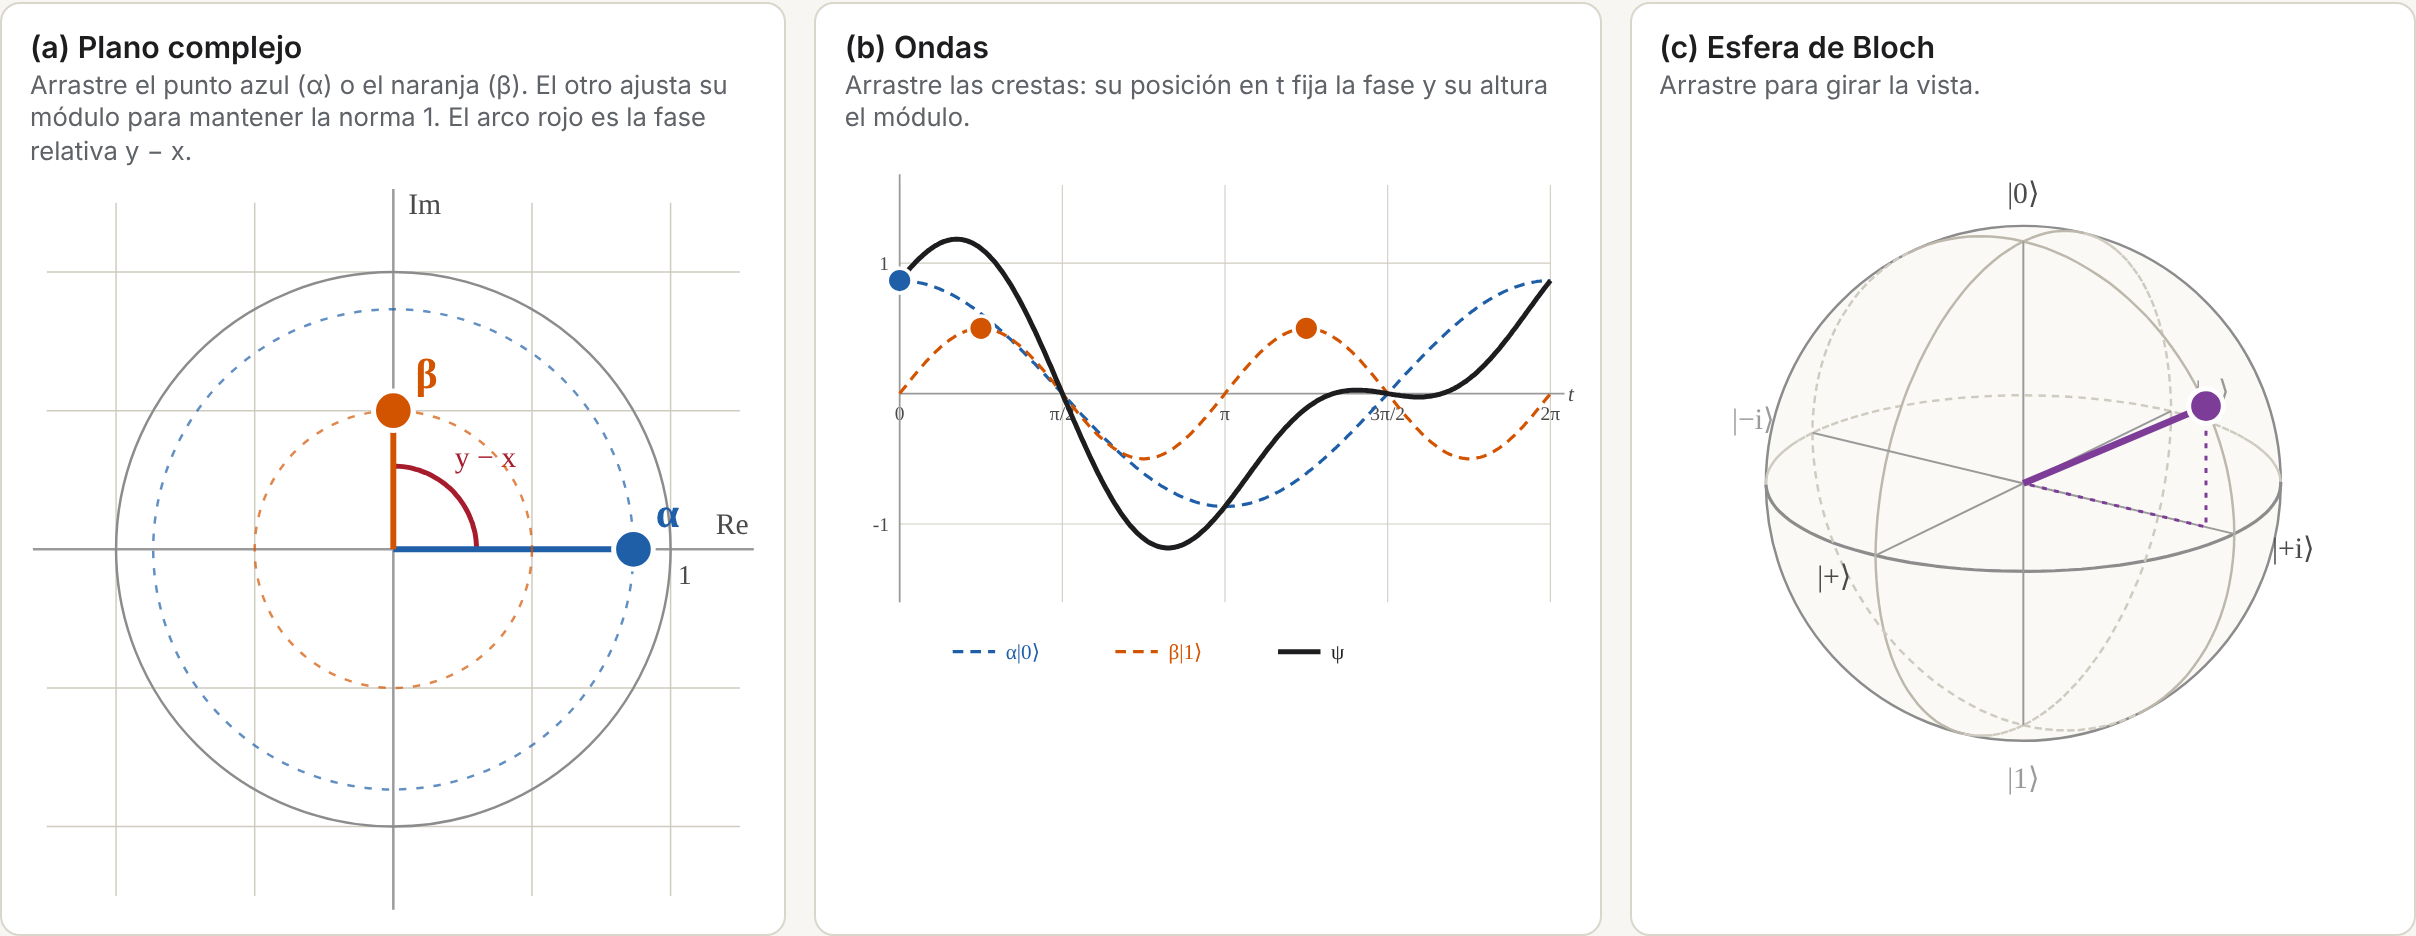
\includegraphics[width=\linewidth]{Imágenes/p13_widget_psi.png}
\caption{El estado $\ket\psi=\frac{\sqrt3}{2}\ket0+\frac{i}{2}\ket1$ en el widget del punto 1.2:
(a) los coeficientes, (b) las ondas y (c) el punto de la esfera de Bloch, con $\theta=60^\circ$
y $\varphi=90^\circ$.}
\label{fig:13-widget-psi}
\end{figure}

\begin{figure}[H]
\centering
\begin{minipage}{0.19\linewidth}\centering
  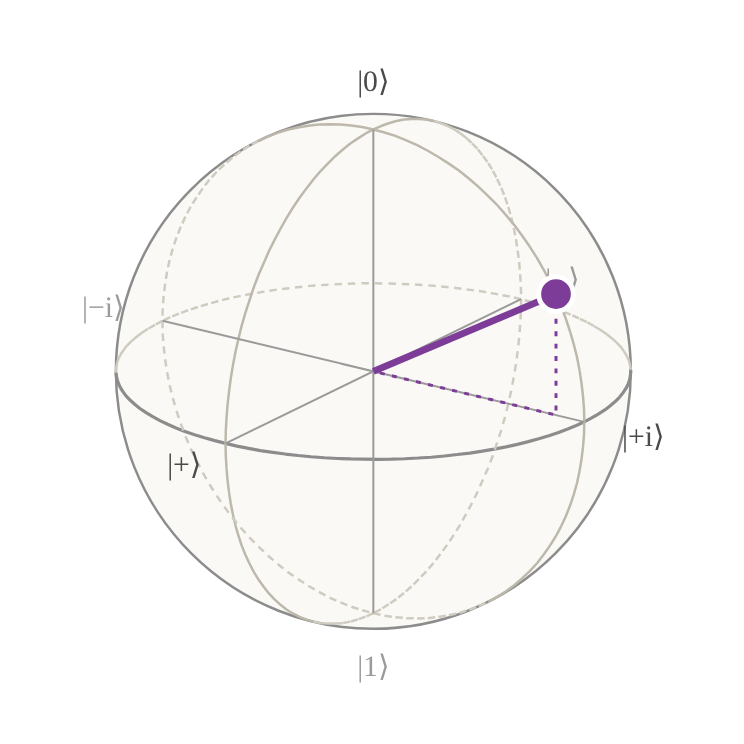
\includegraphics[width=\linewidth]{Imágenes/p13_bloch_psi.png}\\[-2pt]
  {\footnotesize $\ket\psi$\\ $\varphi=90^\circ$}
\end{minipage}\hfill
\begin{minipage}{0.19\linewidth}\centering
  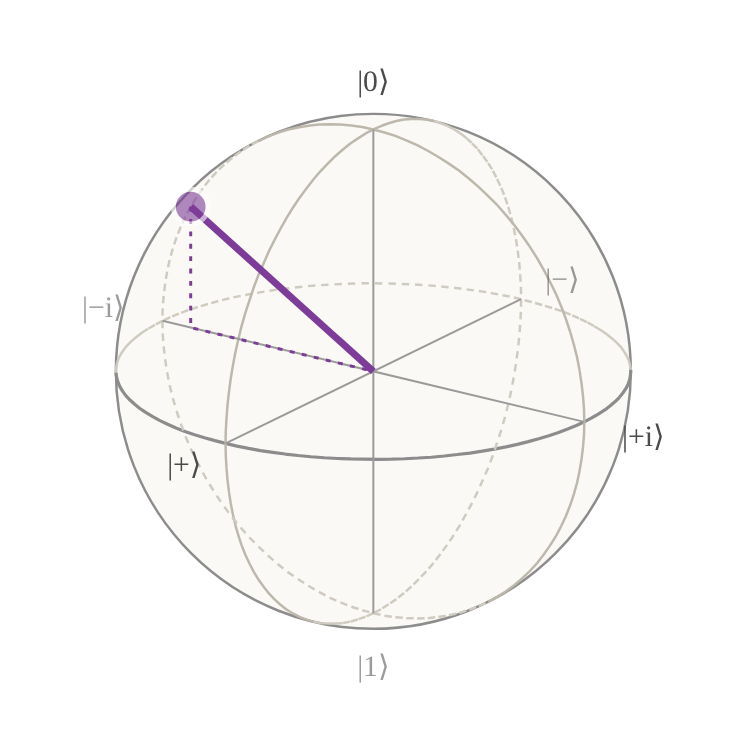
\includegraphics[width=\linewidth]{Imágenes/p13_bloch_tau0.png}\\[-2pt]
  {\footnotesize $\tau=0$\\ $\varphi'=-90^\circ$}
\end{minipage}\hfill
\begin{minipage}{0.19\linewidth}\centering
  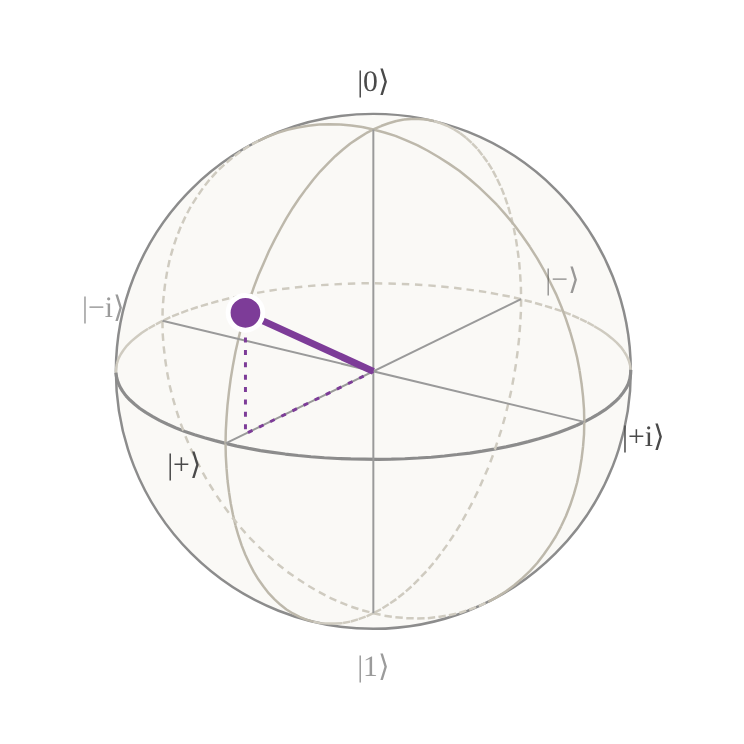
\includegraphics[width=\linewidth]{Imágenes/p13_bloch_taumas.png}\\[-2pt]
  {\footnotesize $\tau=\frac\pi2$\\ $\varphi'=0^\circ$}
\end{minipage}\hfill
\begin{minipage}{0.19\linewidth}\centering
  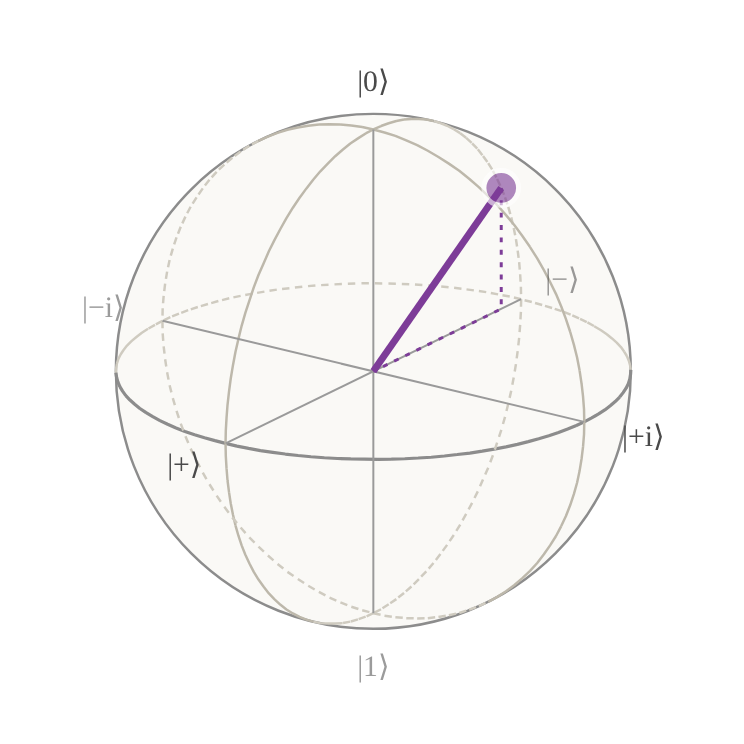
\includegraphics[width=\linewidth]{Imágenes/p13_bloch_taumenos.png}\\[-2pt]
  {\footnotesize $\tau=-\frac\pi2$\\ $\varphi'=180^\circ$}
\end{minipage}\hfill
\begin{minipage}{0.19\linewidth}\centering
  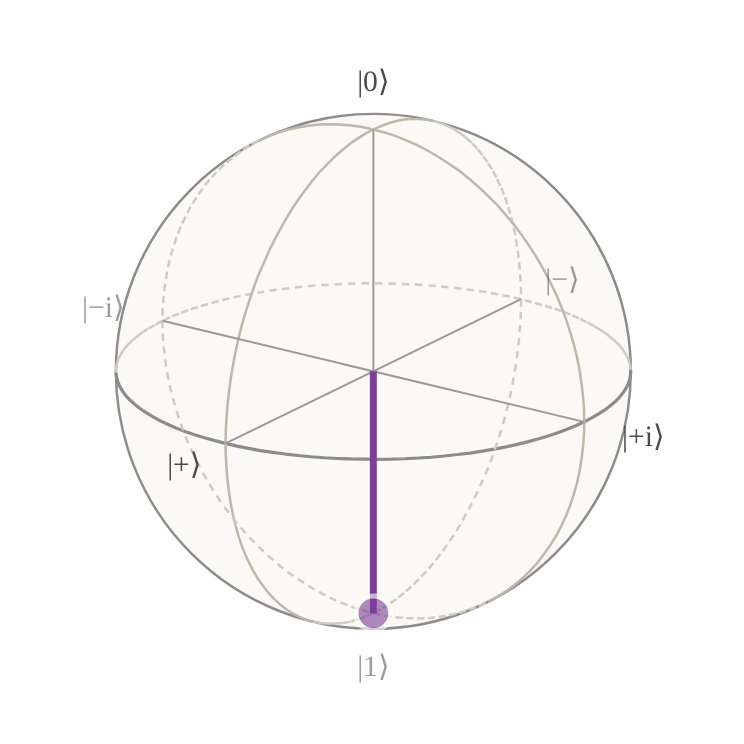
\includegraphics[width=\linewidth]{Imágenes/p13_bloch_final.png}\\[-2pt]
  {\footnotesize estado final\\ $\frac{c}{|c|}\ket1$}
\end{minipage}
\caption{$\ket\psi$, tres soluciones $\ket{\psi'}$ y el estado final en el widget. Los cuatro
primeros están en el mismo paralelo; el estado final es el polo sur.}
\label{fig:13-widget-bloch}
\end{figure}

\color{rojoUN}

\subsection{}

Sean $\ket{\psi}, \ket{\psi'}$ como en el punto anterior y $\rho = \ketbra{\psi}{\psi}$, $\rho' = \ketbra{\psi'}{\psi'}$. Muestre que todo estado mixto $p\rho + (1-p)\rho'$ con $p \in [0,1]$, tiene las mismas probabilidades de medición en la base computacional que $\ket{\psi}$. ¿Qué representa esto en la esfera de Bloch?

\color{Black}

\subsubsection*{Solución.}

\addcontentsline{toc}{subsubsection}{Solución.}

Sean $\ket\psi=\alpha\ket0+\beta\ket1$ y una solución del punto 1.3,
\[
  \ket{\psi'}=\alpha'\ket0+\beta'\ket1=e^{-i\eta}\bigl(-\alpha\ket0+e^{i\tau}\beta\ket1\bigr)
  \quad\eqref{eq:13-soluciones},
\]
que tiene las mismas probabilidades de medición que $\ket\psi$: $|\alpha'|=|\alpha|$ y
$|\beta'|=|\beta|$. En el punto 1.3 se sumaron los kets; en este punto se suman sus proyectores,
que primero se escriben como matrices.

\begin{definicionT}[Bra y proyector de un estado]
Al ket $\ket\psi=\alpha\ket0+\beta\ket1$ se le asocia la matriz columna de sus coordenadas en la
base $\{\ket0,\ket1\}$, y su \emph{bra} $\bra\psi$ es la matriz fila que se obtiene al trasponer
y conjugar esa columna:
\[
  \ket\psi=\begin{pmatrix}\alpha\\ \beta\end{pmatrix},\qquad
  \bra\psi=\begin{pmatrix}\overline\alpha & \overline\beta\end{pmatrix},
\]
donde $\overline z$ es el conjugado de $z$. El \emph{proyector} del estado es el producto de la
columna por la fila,
\begin{equation}\label{eq:14-proyector}
  \rho=\ket\psi\bra\psi
  =\begin{pmatrix}\alpha\\ \beta\end{pmatrix}
   \begin{pmatrix}\overline\alpha & \overline\beta\end{pmatrix}
  =\begin{pmatrix}\alpha\overline\alpha & \alpha\overline\beta\\
                  \beta\overline\alpha & \beta\overline\beta\end{pmatrix}
  =\begin{pmatrix}|\alpha|^2 & \alpha\overline\beta\\
                  \beta\overline\alpha & |\beta|^2\end{pmatrix},
\end{equation}
donde se usó $z\overline z=|z|^2$. Las filas y columnas de $\rho$ se numeran $0$ y $1$, como los
estados de la base, y su entrada en la fila $j$ y la columna $k$ se escribe $\rho_{jk}$.
\end{definicionT}

En la diagonal de $\rho$ están las probabilidades de medición de $\ket\psi$: $\rho_{00}=|\alpha|^2$
es la probabilidad de obtener $0$ y $\rho_{11}=|\beta|^2$ la de obtener $1$. Las fases de $\alpha$
y $\beta$ solo aparecen fuera de la diagonal.

\begin{definicionT}[Estado mixto]
Si $\rho_1,\dots,\rho_n$ son proyectores de estados puros y $p_1,\dots,p_n$ son números reales
con $p_i\ge0$ y $p_1+\dots+p_n=1$, la matriz
\[
  p_1\rho_1+\dots+p_n\rho_n
\]
es un \emph{estado mixto}. Representa un estado probabilístico: el sistema está en el estado
puro de $\rho_i$ con probabilidad $p_i$.
\end{definicionT}

El estado que se estudia en este punto es la mezcla de dos estados,
\begin{equation}\label{eq:14-mezcla}
  \rho_p=p\rho+(1-p)\rho',\qquad \rho=\ket\psi\bra\psi,\quad \rho'=\ket{\psi'}\bra{\psi'},
  \quad p\in[0,1],
\end{equation}
que está en $\ket\psi$ con probabilidad $p$ y en $\ket{\psi'}$ con probabilidad $1-p$.

%======================================================================
\subsection*{Las probabilidades de medición de la mezcla}
%======================================================================

Como la mezcla está en $\ket\psi$ con probabilidad $p$ y en $\ket{\psi'}$ con probabilidad $1-p$,
por la ley de probabilidad total la probabilidad de obtener $0$ es
\[
  P_{\rho_p}(0)=p\,P_\psi(0)+(1-p)\,P_{\psi'}(0)=p\,|\alpha|^2+(1-p)\,|\alpha'|^2
  =p\,|\alpha|^2+(1-p)\,|\alpha|^2=|\alpha|^2 ,
\]
donde se usó $|\alpha'|=|\alpha|$ y $p+(1-p)=1$. Del mismo modo, $P_{\rho_p}(1)=|\beta|^2$. Por tanto,
\[
  \destacado{P_{\rho_p}(0)=|\alpha|^2=P_\psi(0),\qquad P_{\rho_p}(1)=|\beta|^2=P_\psi(1),
  \qquad\text{para todo }p\in[0,1],}
\]
es decir, toda mezcla $p\rho+(1-p)\rho'$ tiene las mismas probabilidades de medición en la base
computacional que $\ket\psi$.

La misma cuenta se ve en las matrices. Por $\rho=\begin{pmatrix}|\alpha|^2 & \alpha\overline\beta\\ \beta\overline\alpha & |\beta|^2\end{pmatrix}$ \eqref{eq:14-proyector}, y como $|\alpha'|=|\alpha|$ y
$|\beta'|=|\beta|$, las matrices $\rho$ y $\rho'$ tienen la misma diagonal, $|\alpha|^2$ y
$|\beta|^2$. Como las matrices se suman y se multiplican por números entrada por entrada,
\begin{equation}\label{eq:14-rho-p}
  \rho_p=\begin{pmatrix}
     |\alpha|^2 & p\,\alpha\overline\beta+(1-p)\,\alpha'\overline{\beta'}\\[2pt]
     p\,\beta\overline\alpha+(1-p)\,\beta'\overline{\alpha'} & |\beta|^2
   \end{pmatrix}.
\end{equation}
La diagonal de $\rho_p$ son las probabilidades de $\ket\psi$ para todo $p$; el número $p$ solo
cambia las entradas de fuera de la diagonal.

\paragraph{Diferencia entre superponer y mezclar.} En el punto 1.3 se sumaron amplitudes, que son
números complejos con fase y se pueden anular: $\alpha+e^{i\eta}\alpha'=0$, y el resultado $0$
desaparece. En una mezcla se suman probabilidades, que son números reales no negativos y no se
anulan: $p|\alpha|^2+(1-p)|\alpha|^2=|\alpha|^2$. Por eso la superposición cambia las
probabilidades y la mezcla no.

%======================================================================
\subsection*{Interpretación en la esfera de Bloch}
%======================================================================

En el punto 1.2 se obtuvo el punto de un estado puro,
$\vec r=\bigl(2\Real(\overline\alpha\beta),\ 2\Imag(\overline\alpha\beta),\ A^2-B^2\bigr)$
\eqref{eq:a-c}. En la matriz $\rho$ se tiene $\rho_{00}=A^2$, $\rho_{11}=B^2$ y
$\rho_{10}=\beta\overline\alpha=\overline\alpha\beta$, así que el punto se lee de las entradas de
la matriz:
\begin{equation}\label{eq:14-bloch-matriz}
  \destacado{r_x=2\,\Real\rho_{10},\qquad
  r_y=2\,\Imag\rho_{10},\qquad
  r_z=\rho_{00}-\rho_{11}.}
\end{equation}
Para un estado mixto se usan las mismas fórmulas con las entradas de $\rho_p$. Como cada entrada
de $\rho_p$ es $p$ por la entrada de $\rho$ más $(1-p)$ por la de $\rho'$, si $\vec r$ y
$\vec r\,'$ son los puntos de $\ket\psi$ y $\ket{\psi'}$,
\begin{equation}\label{eq:14-segmento}
  \destacado{\vec r_p=p\,\vec r+(1-p)\,\vec r\,' ,\qquad p\in[0,1].}
\end{equation}

\begin{definicionT}[Cuerda]
Una \emph{cuerda} de la esfera es el segmento de recta que une dos puntos de su superficie. Sus
puntos, salvo los dos extremos, están en el interior de la esfera.
\end{definicionT}

Por $\vec r_p=p\,\vec r+(1-p)\,\vec r\,'$ \eqref{eq:14-segmento}, con $p=0$ se obtiene
$\vec r\,'$, con $p=1$ se obtiene $\vec r$, y con los valores intermedios se obtienen los puntos
del segmento que los une, más cerca de $\ket\psi$ cuanto mayor es $p$. Es decir, las mezclas
forman la cuerda que une $\ket{\psi'}$ con $\ket\psi$, y por eso quedan dentro de la esfera.
Además, todas tienen la misma altura, $r_z=\rho_{00}-\rho_{11}=|\alpha|^2-|\beta|^2$, porque la
diagonal de $\rho_p$ no depende de $p$. La cuerda es horizontal: une dos puntos del paralelo de
$\ket\psi$ del punto 1.3. Como $\rho_{00}+\rho_{11}=1$ y $\rho_{00}-\rho_{11}=r_z$, las
probabilidades solo dependen de la altura,
\[
  P(0)=\rho_{00}=\frac{1+r_z}{2},\qquad P(1)=\rho_{11}=\frac{1-r_z}{2},
\]
así que todos los puntos de la cuerda tienen las mismas probabilidades que $\ket\psi$. En resumen,
superponer $\ket\psi$ y $\ket{\psi'}$ (punto 1.3) lleva el estado al polo sur, mientras que
mezclarlos lo deja en la cuerda entre los dos, dentro de la esfera y a la misma altura.

%======================================================================
\subsection*{Comprobación con el ejemplo del punto 1.3}
%======================================================================

Se toma el ejemplo del punto 1.3, $\ket\psi=\frac{\sqrt3}{2}\ket0+\frac{i}{2}\ket1$, es decir,
$\alpha=\frac{\sqrt3}{2}$ y $\beta=\frac{i}{2}$, y la solución con $\tau=0$ y $\eta=0$,
$\ket{\psi'}=-\frac{\sqrt3}{2}\ket0+\frac{i}{2}\ket1$, es decir, $\alpha'=-\frac{\sqrt3}{2}$ y
$\beta'=\frac{i}{2}$.

\paragraph{Proyectores.} Como el conjugado de $\frac{i}{2}$ es $-\frac{i}{2}$, por
$\rho=\begin{pmatrix}|\alpha|^2 & \alpha\overline\beta\\ \beta\overline\alpha & |\beta|^2\end{pmatrix}$ \eqref{eq:14-proyector} las entradas de $\rho$ son
\[
  \rho_{00}=\tfrac34,\qquad
  \rho_{01}=\tfrac{\sqrt3}{2}\bigl(-\tfrac{i}{2}\bigr)=-\tfrac{\sqrt3}{4}i,\qquad
  \rho_{10}=\tfrac{i}{2}\cdot\tfrac{\sqrt3}{2}=\tfrac{\sqrt3}{4}i,\qquad
  \rho_{11}=\tfrac14 .
\]
En $\rho'$ solo cambia el signo de $\alpha$, así que la diagonal es la misma y cambia el signo de
las otras dos entradas: $\rho'_{01}=\bigl(-\tfrac{\sqrt3}{2}\bigr)\bigl(-\tfrac{i}{2}\bigr)=\tfrac{\sqrt3}{4}i$ y
$\rho'_{10}=\tfrac{i}{2}\bigl(-\tfrac{\sqrt3}{2}\bigr)=-\tfrac{\sqrt3}{4}i$. Entonces
\[
  \rho=\begin{pmatrix}\frac34 & -\frac{\sqrt3}{4}i\\[3pt] \frac{\sqrt3}{4}i & \frac14\end{pmatrix},
  \qquad
  \rho'=\begin{pmatrix}\frac34 & \frac{\sqrt3}{4}i\\[3pt] -\frac{\sqrt3}{4}i & \frac14\end{pmatrix}.
\]

\paragraph{Mezcla.} Al calcular $p\rho+(1-p)\rho'$ entrada por entrada, la diagonal queda
$p\cdot\frac34+(1-p)\cdot\frac34=\frac34$ y $p\cdot\frac14+(1-p)\cdot\frac14=\frac14$, y
\[
  (\rho_p)_{10}=p\cdot\tfrac{\sqrt3}{4}i+(1-p)\bigl(-\tfrac{\sqrt3}{4}i\bigr)=(2p-1)\tfrac{\sqrt3}{4}i ,
\]
y $(\rho_p)_{01}$ es su conjugado. Por tanto
\[
  \rho_p=\begin{pmatrix}\frac34 & -(2p-1)\frac{\sqrt3}{4}i\\[3pt]
                        (2p-1)\frac{\sqrt3}{4}i & \frac14\end{pmatrix}.
\]
Por ejemplo, con $p=\frac14$ se tiene $2p-1=-\frac12$, y
$\rho_{1/4}=\begin{pmatrix}\frac34 & \frac{\sqrt3}{8}i\\[2pt] -\frac{\sqrt3}{8}i & \frac14\end{pmatrix}$.

\paragraph{Probabilidades.} La diagonal no depende de $p$: para toda mezcla, $P(0)=\frac34$ y
$P(1)=\frac14$, que son las probabilidades de $\ket\psi$, pues $|\alpha|^2=\frac34$ y
$|\beta|^2=\frac14$. Esto comprueba en el ejemplo el resultado general; en el punto 1.5 se
comprueba también con mediciones simuladas.

\paragraph{Punto en la esfera.} El número $(\rho_p)_{10}=(2p-1)\frac{\sqrt3}{4}i$ tiene parte real
$0$ y parte imaginaria $(2p-1)\frac{\sqrt3}{4}$. Por
$r_x=2\,\Real\rho_{10},\ r_y=2\,\Imag\rho_{10},\ r_z=\rho_{00}-\rho_{11}$ \eqref{eq:14-bloch-matriz},
\[
  \vec r_p=\Bigl(0,\ (2p-1)\tfrac{\sqrt3}{2},\ \tfrac34-\tfrac14\Bigr)
          =\Bigl(0,\ (2p-1)\tfrac{\sqrt3}{2},\ \tfrac12\Bigr).
\]
\begin{center}
\renewcommand{\arraystretch}{1.45}
\begin{tabular}{cccc}
  $p$ & $\vec r_p$ & $P(0)$ & $P(1)$\\\hline
  $0$ & $\bigl(0,-\frac{\sqrt3}{2},\frac12\bigr)$, punto de $\ket{\psi'}$ & $\frac34$ & $\frac14$\\
  $\frac14$ & $\bigl(0,-\frac{\sqrt3}{4},\frac12\bigr)$ & $\frac34$ & $\frac14$\\
  $\frac12$ & $\bigl(0,0,\frac12\bigr)$, sobre el eje $z$ & $\frac34$ & $\frac14$\\
  $\frac34$ & $\bigl(0,\frac{\sqrt3}{4},\frac12\bigr)$ & $\frac34$ & $\frac14$\\
  $1$ & $\bigl(0,\frac{\sqrt3}{2},\frac12\bigr)$, punto de $\ket{\psi}$ & $\frac34$ & $\frac14$
\end{tabular}
\end{center}
Con $p=0$ y $p=1$ se obtienen los puntos de $\ket{\psi'}$ y de $\ket\psi$,
$(0,-0.866,0.5)$ y $(0,0.866,0.5)$, que son los que muestra el widget. Los demás están en la
cuerda que los une, a altura $\frac12$. Como en este caso $\ket{\psi'}$ está enfrente de
$\ket\psi$ en el paralelo, la cuerda pasa por el eje $z$, en $p=\frac12$ (figura~\ref{fig:14-bloch},
izquierda).

Con la solución de $\tau=\frac\pi2$ del punto 1.3, $\ket{\psi'}=-\frac{\sqrt3}{2}\ket0-\frac12\ket1$,
se tiene $\rho'_{10}=\bigl(-\frac12\bigr)\bigl(-\frac{\sqrt3}{2}\bigr)=\frac{\sqrt3}{4}$, así que
$(\rho_p)_{10}=p\frac{\sqrt3}{4}i+(1-p)\frac{\sqrt3}{4}$ y
\[
  \vec r_p=\Bigl((1-p)\tfrac{\sqrt3}{2},\ p\,\tfrac{\sqrt3}{2},\ \tfrac12\Bigr),
\]
que es otra cuerda del mismo paralelo, entre $(0.866,0,0.5)$ y $(0,0.866,0.5)$
(figura~\ref{fig:14-bloch}, derecha).

\begin{figure}[H]
\centering
\begin{minipage}{0.42\linewidth}\centering
  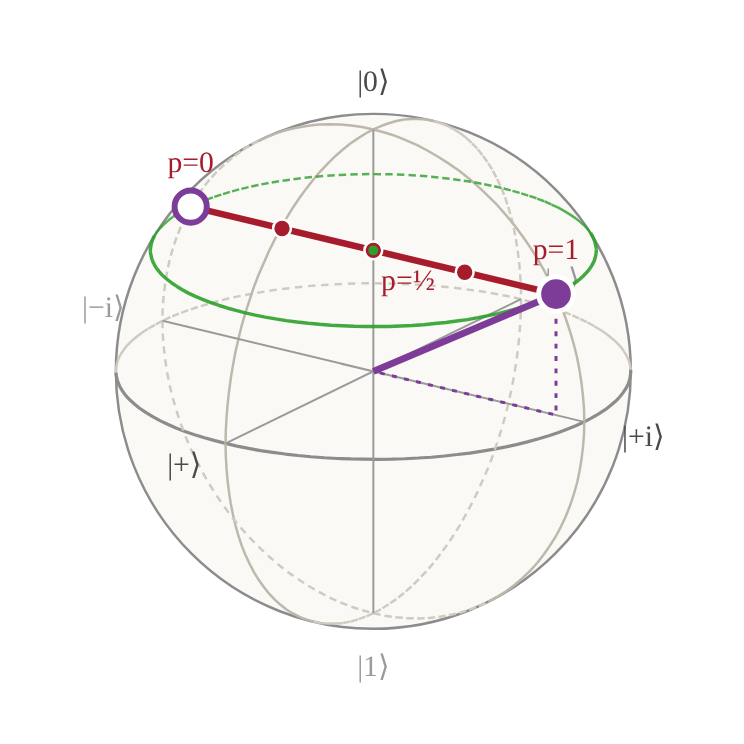
\includegraphics[width=\linewidth]{Imágenes/p14_mezcla_tau0.png}\\
  {\footnotesize $\ket{\psi'}$ con $\tau=0$}
\end{minipage}\hspace{0.06\linewidth}
\begin{minipage}{0.42\linewidth}\centering
  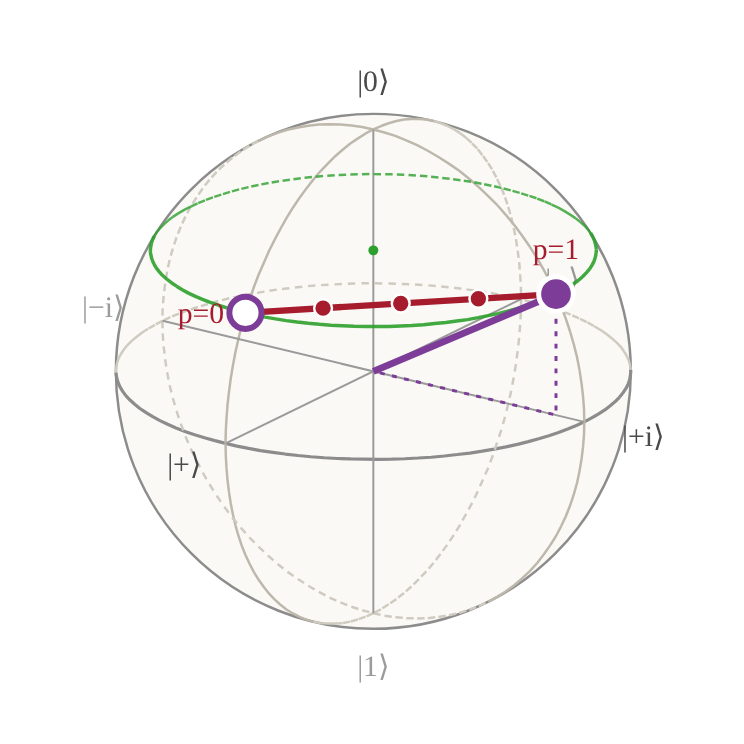
\includegraphics[width=\linewidth]{Imágenes/p14_mezcla_taupi2.png}\\
  {\footnotesize $\ket{\psi'}$ con $\tau=\frac\pi2$}
\end{minipage}
\caption{Panel (c) del widget con el estado $\ket\psi$ (punto morado relleno). Sobre la captura
se marcaron, con las coordenadas calculadas arriba, el punto de $\ket{\psi'}$ (círculo morado
vacío), el paralelo de altura $\frac12$ (verde) y los estados mixtos $\rho_p$ para
$p=0,\frac14,\frac12,\frac34,1$ (rojo). Las mezclas forman la cuerda que une $\ket{\psi'}$
($p=0$) con $\ket\psi$ ($p=1$), dentro de la esfera y a la misma altura.}
\label{fig:14-bloch}
\end{figure}


\color{rojoUN}

\subsection{}

Implemente en Qiskit, para un $\ket{\psi}$ arbitrario:
    \begin{enumerate}[label=(\alph*)]
        \item la construcción de $\ket{\psi'}$ y $\eta$ del punto 1.3, verificando que $\ket{\psi}$ y $\ket{\psi'}$ tienen las mismas probabilidades de medición y que $\ket{\psi} + e^{i\eta}\ket{\psi'}$, normalizado, coincide con $\ket{1}$ salvo fase global;
        \item el estado $p\rho + (1-p)\rho'$ del punto 1.4 para varios valores de $p$, con sus probabilidades de medición;
        \item los vectores de Bloch de todos los estados anteriores, comparándolos con los de su widget.
    \end{enumerate}
    En (a) y (b) reporte tanto las probabilidades exactas como las frecuencias obtenidas en mediciones simuladas.

\color{Black}

\subsubsection*{Solución.}

\addcontentsline{toc}{subsubsection}{Solución.}

Los puntos 1.3 y 1.4 se implementaron en el notebook \texttt{punto\_1\_5\_qiskit.ipynb}, con las
herramientas que se usan en el curso de IBM Quantum Learning (\emph{Basics of quantum
information}): \texttt{Statevector} para los estados puros, \texttt{DensityMatrix} para los
proyectores y los estados mixtos, y circuitos de \texttt{QuantumCircuit} que se corren con el
\texttt{StatevectorSampler} para simular mediciones. Las funciones reciben $\alpha$ y $\beta$
cualesquiera; en este documento se reportan los resultados para el estado de los puntos 1.3 y
1.4,
\[
  \ket\psi=\tfrac{\sqrt3}{2}\ket0+\tfrac{i}{2}\ket1 ,
\]
y al final del notebook se repiten todas las comprobaciones con $200$ estados, valores de $\tau$,
$\eta$ y $p$ elegidos al azar.

\paragraph{Probabilidades exactas y frecuencias.}
Las probabilidades exactas se calculan con la regla de Born, que en Qiskit es el método
\texttt{probabilities\_dict()}: para un \texttt{Statevector} da $|\alpha|^2$ y $|\beta|^2$, y
para una \texttt{DensityMatrix} da la diagonal de la matriz. Para las mediciones simuladas se
arma un circuito de un qubit que prepara el estado con \texttt{initialize} y lo mide en la base
computacional, y se corre $N=4000$ veces. La frecuencia del resultado $0$ es una proporción
muestral, así que su desviación estándar es
\[
  \sqrt{\frac{P(0)\bigl(1-P(0)\bigr)}{N}}=\sqrt{\frac{0.75\cdot0.25}{4000}}\approx0.007 ,
\]
y las diferencias entre las frecuencias y las probabilidades exactas deben ser de ese orden.

%======================================================================
\subsection*{(a) Construcción de $\ket{\psi'}$ y $\eta$}
%======================================================================

La función \texttt{construir\_psi\_prima} aplica las fórmulas del punto 1.3,
\[
  \alpha'=-e^{-i\eta}\alpha,\qquad \beta'=e^{-i\eta}e^{i\tau}\beta,\qquad c=\beta\,(1+e^{i\tau}),
\]
y devuelve un error si $\beta=0$ (no hay solución) o si $\tau=\pm\pi$ (daría $c=0$). Se
probaron las tres soluciones del ejemplo del punto 1.3 con $\eta=0$ y una con $\eta=1$:

\begin{center}
\renewcommand{\arraystretch}{1.3}
\begin{tabular}{lcccc}
  Estado & $P(0)$ exacta & frecuencia de $0$ & $P(1)$ exacta & frecuencia de $1$\\\hline
  $\ket\psi$ & $0.75$ & $0.7555$ & $0.25$ & $0.2445$\\
  $\ket{\psi'}$, $\tau=0$ & $0.75$ & $0.7452$ & $0.25$ & $0.2547$\\
  $\ket{\psi'}$, $\tau=\frac\pi2$ & $0.75$ & $0.7418$ & $0.25$ & $0.2582$\\
  $\ket{\psi'}$, $\tau=-\frac\pi2$ & $0.75$ & $0.7620$ & $0.25$ & $0.2380$\\
  $\ket{\psi'}$, $\tau=0$, $\eta=1$ & $0.75$ & $0.7570$ & $0.25$ & $0.2430$
\end{tabular}
\end{center}

Todas las $\ket{\psi'}$ tienen exactamente las probabilidades de $\ket\psi$, y las frecuencias
quedan a menos de dos desviaciones estándar de ellas. Luego se calculó
$\ket\psi+e^{i\eta}\ket{\psi'}$, se normalizó y se comparó con $\ket1$ con el método
\texttt{equiv}, que dice si dos estados son iguales salvo fase global:

\begin{center}
\renewcommand{\arraystretch}{1.3}
\begin{tabular}{lccccc}
  Solución & $\ket\psi+e^{i\eta}\ket{\psi'}$ & norma & $|c|$ & ¿es $\ket1$ salvo fase? & frecuencia de $1$\\\hline
  $\tau=0$ & $(0,\ i)$ & $1$ & $1$ & sí & $1$\\
  $\tau=\frac\pi2$ & $(0,\ -0.5+0.5i)$ & $0.7071$ & $0.7071$ & sí & $1$\\
  $\tau=-\frac\pi2$ & $(0,\ 0.5+0.5i)$ & $0.7071$ & $0.7071$ & sí & $1$\\
  $\tau=0$, $\eta=1$ & $(0,\ i)$ & $1$ & $1$ & sí & $1$
\end{tabular}
\end{center}

La coordenada de $\ket0$ de la suma es $0$ en todos los casos, la norma de la suma es $|c|$
porque la suma es $c\ket1$, y al medir el estado normalizado solo se obtiene $1$. Los valores de
$c$ son los mismos de la tabla del punto 1.3. La solución con $\eta=1$ da la misma suma que con
$\eta=0$, porque $\eta$ solo compensa la fase global con la que se escribe $\ket{\psi'}$.

%======================================================================
\subsection*{(b) El estado mixto $p\rho+(1-p)\rho'$}
%======================================================================

Con la solución de $\tau=0$, $\ket{\psi'}=-\frac{\sqrt3}{2}\ket0+\frac{i}{2}\ket1$, se construyeron
$\rho$ y $\rho'$ con \texttt{DensityMatrix}, que calcula el proyector $\ket\psi\bra\psi$ a partir
del ket, y las mezclas $\rho_p=p\rho+(1-p)\rho'$ para $p=0,\frac14,\frac12,\frac34,1$. Las matrices
que se obtienen son las del punto 1.4; por ejemplo, para $p=\frac14$,
\[
  \rho_{1/4}=\begin{pmatrix}0.75 & 0.2165\,i\\ -0.2165\,i & 0.25\end{pmatrix},
\]
que coincide con $\rho_p$ del punto 1.4 para $p=\frac14$, pues
$-(2p-1)\frac{\sqrt3}{4}=\frac{\sqrt3}{8}\approx0.2165$.

Para simular las mediciones de la mezcla se usó lo que significa un estado mixto: en cada
medición el qubit está en $\ket\psi$ con probabilidad $p$ y en $\ket{\psi'}$ con probabilidad
$1-p$. Por eso, de las $N$ mediciones, el número que se hace con $\ket\psi$ es una variable
binomial con parámetros $N$ y $p$. Se generó ese número, se corrieron esas mediciones con el
circuito de $\ket\psi$ y las demás con el de $\ket{\psi'}$, y se juntaron los conteos:

\begin{center}
\renewcommand{\arraystretch}{1.3}
\begin{tabular}{ccccc}
  $p$ & $P(0)$ exacta & frecuencia de $0$ & $P(1)$ exacta & frecuencia de $1$\\\hline
  $0$ & $0.75$ & $0.7635$ & $0.25$ & $0.2365$\\
  $\frac14$ & $0.75$ & $0.7560$ & $0.25$ & $0.2440$\\
  $\frac12$ & $0.75$ & $0.7642$ & $0.25$ & $0.2358$\\
  $\frac34$ & $0.75$ & $0.7380$ & $0.25$ & $0.2620$\\
  $1$ & $0.75$ & $0.7505$ & $0.25$ & $0.2495$
\end{tabular}
\end{center}

Para todo $p$ las probabilidades exactas son las de $\ket\psi$, como se mostró en el punto 1.4, y
las frecuencias quedan cerca de ellas: la diferencia más grande, en $p=\frac12$, es de unas
$2.1$ desviaciones estándar.

%======================================================================
\subsection*{(c) Vectores de Bloch}
%======================================================================

Los vectores se calcularon con las fórmulas del punto 1.4, que leen el punto de la esfera de las
entradas de la matriz,
\[
  r_x=2\,\bigl(\text{parte real de }\rho_{10}\bigr),\qquad
  r_y=2\,\bigl(\text{parte imaginaria de }\rho_{10}\bigr),\qquad
  r_z=\rho_{00}-\rho_{11},
\]
y se compararon con la lectura \emph{r} que muestra el widget del punto 1.2 para cada estado
puro (las capturas del punto 1.3):

\begin{center}
\renewcommand{\arraystretch}{1.3}
\begin{tabular}{lccc}
  Estado & Qiskit & Widget & $|\vec r|$\\\hline
  $\ket\psi$ & $(0,\ 0.866,\ 0.5)$ & $(0,\ 0.866,\ 0.5)$ & $1$\\
  $\ket{\psi'}$, $\tau=0$ & $(0,\ -0.866,\ 0.5)$ & $(0,\ -0.866,\ 0.5)$ & $1$\\
  $\ket{\psi'}$, $\tau=\frac\pi2$ & $(0.866,\ 0,\ 0.5)$ & $(0.866,\ 0,\ 0.5)$ & $1$\\
  $\ket{\psi'}$, $\tau=-\frac\pi2$ & $(-0.866,\ 0,\ 0.5)$ & $(-0.866,\ 0,\ 0.5)$ & $1$\\
  estado final $\ket1$ & $(0,\ 0,\ -1)$ & $(0,\ 0,\ -1)$ & $1$\\\hline
  $\rho_p$, $p=0$ & $(0,\ -0.866,\ 0.5)$ & -- & $1$\\
  $\rho_p$, $p=\frac14$ & $(0,\ -0.433,\ 0.5)$ & -- & $0.6614$\\
  $\rho_p$, $p=\frac12$ & $(0,\ 0,\ 0.5)$ & -- & $0.5$\\
  $\rho_p$, $p=\frac34$ & $(0,\ 0.433,\ 0.5)$ & -- & $0.6614$\\
  $\rho_p$, $p=1$ & $(0,\ 0.866,\ 0.5)$ & -- & $1$
\end{tabular}
\end{center}

Los vectores de los estados puros coinciden con los del widget, que muestra tres decimales. El
widget solo representa estados puros, así que para las mezclas la comparación se hace con los
valores calculados en el punto 1.4, $\vec r_p=\bigl(0,(2p-1)\frac{\sqrt3}{2},\frac12\bigr)$, que
dan los mismos números. Todos los estados, salvo el final, tienen $r_z=0.5$: los estados puros
están en el paralelo de $\ket\psi$ ($|\vec r|=1$) y las mezclas con $0<p<1$ están en la cuerda
que une $\ket{\psi'}$ con $\ket\psi$, dentro de la esfera ($|\vec r|<1$). La
figura~\ref{fig:15-bloch} compara el dibujo de Qiskit con la figura del punto 1.4, que muestra la misma cuerda.

\begin{figure}[htbp]
\centering
\begin{minipage}{0.44\linewidth}\centering
  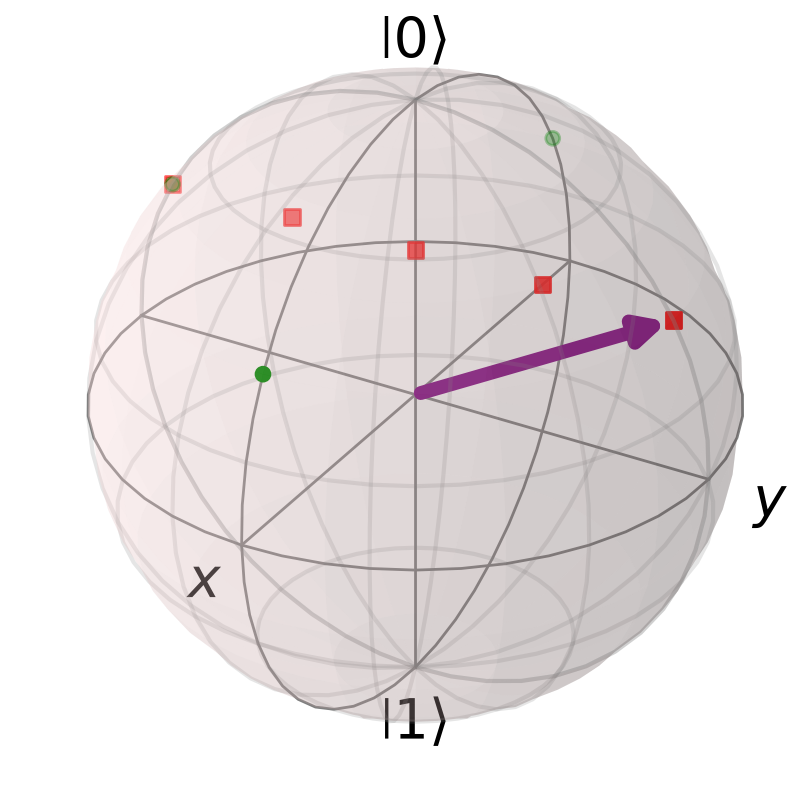
\includegraphics[width=\linewidth]{Imágenes/p15_bloch_qiskit.png}\\
  {\footnotesize Qiskit}
\end{minipage}\hspace{0.04\linewidth}
\begin{minipage}{0.44\linewidth}\centering
  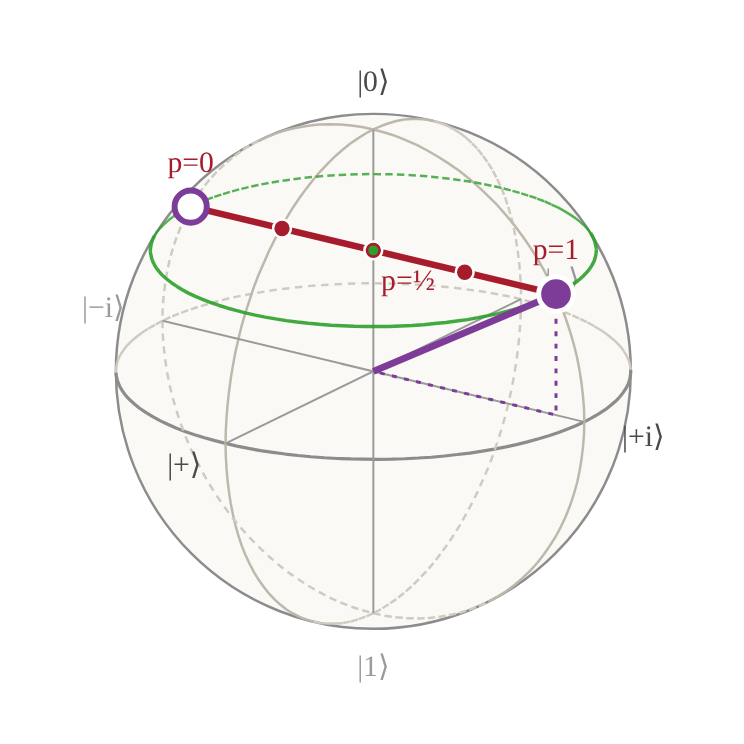
\includegraphics[width=\linewidth]{Imágenes/p14_mezcla_tau0.png}\\
  {\footnotesize Figura del punto 1.4}
\end{minipage}
\caption{A la izquierda, la esfera de Bloch dibujada con la clase \texttt{Bloch} de Qiskit: el
vector de $\ket\psi$ (morado), las tres soluciones $\ket{\psi'}$ del punto 1.3 (verde) y las
mezclas $\rho_p$ con la solución de $\tau=0$ (rojo). A la derecha, la figura del punto 1.4 con
la misma cuerda, porque el widget solo muestra estados puros. En las dos, los puntos de las mezclas quedan sobre el segmento horizontal entre
$\ket{\psi'}$ y $\ket\psi$, a altura $0.5$.}
\label{fig:15-bloch}
\end{figure}


\color{rojoUN}

\section{Ondas de dos variables}

Sean
\[
H_1 = \text{span}_{\C}\{e^{it}, e^{2it}\} \subset L^2([0,2\pi]), \quad H_2 = \text{span}_{\C}\{e^{i(nt+ms)} : n,m=1,2\} \subset L^2([0,2\pi]^2),
\]
con los productos internos de $L^2$ normalizados de modo que las exponenciales sean ortonormales.

\subsection{}

Muestre que $(\psi,\varphi) \mapsto \psi(t)\varphi(s)$ induce un isomorfismo $H_1 \otimes H_1 \cong H_2$. ¿Qué ocurre si, como en la sección anterior, se usan ondas reales en lugar de complejas?

\color{Black}

\subsubsection*{Solución.}

\addcontentsline{toc}{subsubsection}{Solución.}

\paragraph{Los espacios $H_1$ y $H_2$.} Por la fórmula de Euler, para todo número real $x$,
\[
  e^{ix}=\cos x+i\sin x ,
\]
así que $e^{int}=\cos nt+i\sin nt$ es una onda con valores complejos: su parte real es $\cos nt$ y su parte imaginaria es $\sin nt$. El número $n$ es su frecuencia. La notación $\spanC\{f_1,\dots,f_k\}$ denota el conjunto de todas las combinaciones lineales $c_1f_1+\dots+c_kf_k$ con coeficientes $c_1,\dots,c_k\in\C$. Es la misma definición de conjunto generado del punto 1.1, pero con coeficientes complejos en lugar de reales. Así,
\[
  H_1=\{\alpha\,e^{it}+\beta\,e^{2it} : \alpha,\beta\in\C\}.
\]
Para recordar que $H_1$ hace el papel de un qubit, se escribe
\[
  \ket0:=e^{it},\qquad \ket1:=e^{2it},
\]
de modo que un elemento de $H_1$ es $\alpha\ket0+\beta\ket1$, igual que un estado de un qubit.

Del mismo modo, $H_2$ es el conjunto de las combinaciones lineales con coeficientes complejos de las cuatro funciones de dos variables $e^{i(nt+ms)}$ con $n,m\in\{1,2\}$:
\[
  e^{i(t+s)},\qquad e^{i(t+2s)},\qquad e^{i(2t+s)},\qquad e^{i(2t+2s)}.
\]
Por la definición de $H_2$, estas cuatro funciones lo generan: todo elemento de $H_2$ es una combinación lineal de ellas. Los símbolos $L^2([0,2\pi])$ y $L^2([0,2\pi]^2)$ del enunciado denotan los espacios de funciones definidas en $[0,2\pi]$ y en el cuadrado $[0,2\pi]\times[0,2\pi]$ para las que la integral de $|f|^2$ es finita. $H_1$ y $H_2$ están contenidos en ellos y toman de ellos su producto interno.

\begin{definicionT}[Producto interno normalizado]
Para $f,g\in H_1$ se define
\[
  \bk{f}{g}=\frac1{2\pi}\int_0^{2\pi}\overline{f(t)}\,g(t)\,dt ,
\]
y para $F,G\in H_2$,
\[
  \bk{F}{G}=\frac1{4\pi^2}\int_0^{2\pi}\!\!\int_0^{2\pi}\overline{F(t,s)}\,G(t,s)\,dt\,ds .
\]
La notación $\bk{f}{g}$ es la notación de Dirac para el producto interno: a la izquierda va el vector que se conjuga (el \emph{bra}) y a la derecha el otro (el \emph{ket}). Para los kets $\ket0$ y $\ket1$ se abrevia, por ejemplo, $\bk{0}{1}$ en lugar de $\bk{e^{it}}{e^{2it}}$.
\end{definicionT}

La barra sobre $f(t)$ indica el conjugado complejo. Se conjuga la primera función para que $\bk{f}{f}=\frac1{2\pi}\int_0^{2\pi}|f(t)|^2\,dt$ sea un número real mayor o igual que $0$, que sirve para medir el tamaño de $f$: la \emph{norma} de $f$ es $\|f\|=\sqrt{\bk{f}{f}}$. El factor $\frac1{2\pi}$ es la normalización que pide el enunciado. Como $|e^{it}|^2=\cos^2t+\sin^2t=1$, sin ese factor se tendría $\int_0^{2\pi}|e^{it}|^2\,dt=2\pi$, y la norma de $e^{it}$ sería $\sqrt{2\pi}$ en lugar de $1$. Con el factor, $\ket0$ y $\ket1$ tienen norma $1$, como los vectores de la base de un qubit. Por la misma razón, en $H_2$ se divide entre $(2\pi)^2=4\pi^2$, que es el área del cuadrado $[0,2\pi]\times[0,2\pi]$.

\begin{definicionT}[Conjunto ortonormal]
Un conjunto de funciones $\{f_1,\dots,f_k\}$ es \emph{ortonormal} si $\bk{f_j}{f_j}=1$ para cada $j$ (cada función tiene norma $1$) y $\bk{f_j}{f_l}=0$ cuando $j\neq l$. La segunda condición se expresa diciendo que las funciones son \emph{ortogonales dos a dos}: cada pareja de funciones distintas del conjunto tiene producto interno $0$.
\end{definicionT}

\paragraph{Ortonormalidad en $H_1$.} En el punto 1.1 se obtuvo
\[
  \int_0^{2\pi}\cos(kt)\,dt=\begin{cases}2\pi,&k=0,\\0,&k\neq0,\end{cases}\qquad
  \int_0^{2\pi}\sin(kt)\,dt=0\quad\text{para todo entero }k .
\]
Con la fórmula de Euler, para un entero $k$,
\[
  \frac1{2\pi}\int_0^{2\pi}e^{ikt}\,dt=\frac1{2\pi}\Bigl(\int_0^{2\pi}\cos(kt)\,dt+i\int_0^{2\pi}\sin(kt)\,dt\Bigr)=\begin{cases}1,&k=0,\\0,&k\neq0.\end{cases}
\]
Como $\overline{e^{ipt}}=\cos pt-i\sin pt=e^{-ipt}$ y $e^{-ipt}e^{iqt}=e^{i(q-p)t}$, para enteros $p$ y $q$ se tiene
\[
  \bk{e^{ipt}}{e^{iqt}}=\frac1{2\pi}\int_0^{2\pi}e^{i(q-p)t}\,dt=\begin{cases}1,&p=q,\\0,&p\neq q.\end{cases}
\]
Con $p,q\in\{1,2\}$ resulta $\bk{0}{0}=\bk{1}{1}=1$ y $\bk{0}{1}=\bk{1}{0}=0$, así que $\{\ket0,\ket1\}$ es ortonormal.

Un conjunto ortonormal siempre es linealmente independiente. Si $c_1f_1+\dots+c_kf_k=0$, se hace el producto interno con $f_j$ a ambos lados. Como el producto interno es lineal en la segunda entrada, queda $c_1\bk{f_j}{f_1}+\dots+c_k\bk{f_j}{f_k}=0$. Todos los términos son $0$ salvo el de $f_j$, que vale $c_j\cdot1$, así que $c_j=0$ para cada $j$. Por tanto $\ket0$ y $\ket1$ son linealmente independientes y forman una base de $H_1$, de modo que $\dim_{\C}H_1=2$. En particular, $H_1$ es un espacio de Hilbert, es decir, un espacio vectorial complejo con producto interno, de dimensión $2$.

\paragraph{Ortonormalidad en $H_2$.} En una integral doble de una función de la forma $f(t)g(s)$, al integrar en $t$ con $s$ fija, $g(s)$ es una constante y sale de la integral. Por eso
\[
  \int_0^{2\pi}\!\!\int_0^{2\pi}f(t)\,g(s)\,dt\,ds=\Bigl(\int_0^{2\pi}f(t)\,dt\Bigr)\Bigl(\int_0^{2\pi}g(s)\,ds\Bigr).
\]
Como $\overline{e^{i(nt+ms)}}=e^{-int}e^{-ims}$, para $n,m,n',m'\in\{1,2\}$,
\[
  \bk{e^{i(nt+ms)}}{e^{i(n't+m's)}}=\Bigl(\frac1{2\pi}\int_0^{2\pi}e^{i(n'-n)t}\,dt\Bigr)\Bigl(\frac1{2\pi}\int_0^{2\pi}e^{i(m'-m)s}\,ds\Bigr).
\]
Esto vale $1$ si $n=n'$ y $m=m'$, y $0$ en cualquier otro caso. Así, las cuatro funciones son ortonormales; por lo anterior son linealmente independientes, y como generan $H_2$, forman una base de $H_2$. Por tanto $\dim_{\C}H_2=4$.

\begin{definicionT}[Producto tensorial]
Como se vio en clase, $H_1\otimes H_1$ es el espacio vectorial complejo cuya base ortonormal son los cuatro símbolos
\[
  \ket0\otimes\ket0,\qquad \ket0\otimes\ket1,\qquad \ket1\otimes\ket0,\qquad \ket1\otimes\ket1 ,
\]
es decir, $\ket a\otimes\ket b$ con $a,b\in\{0,1\}$. Sus elementos son las combinaciones $\sum_{a,b}c_{ab}\,\ket a\otimes\ket b$ con $c_{ab}\in\C$, y su dimensión es $2\cdot2=4$. Para $\psi=x_0\ket0+x_1\ket1$ y $\varphi=y_0\ket0+y_1\ket1$ en $H_1$ se define
\[
  \psi\otimes\varphi=\sum_{a,b\in\{0,1\}}x_a\,y_b\,\ket a\otimes\ket b :
\]
el coeficiente de cada pareja $\ket a\otimes\ket b$ es el producto de los coeficientes.
\end{definicionT}

Con esta definición, un número complejo $c$ se puede sacar de cualquiera de los dos factores: multiplicar $\psi$ por $c$ multiplica todos los $x_a$ por $c$, y multiplicar $\varphi$ por $c$ multiplica todos los $y_b$ por $c$. En ambos casos todos los coeficientes $x_ay_b$ quedan multiplicados por $c$, así que
\[
  (c\,\psi)\otimes\varphi=c\,(\psi\otimes\varphi)=\psi\otimes(c\,\varphi).
\]
Del mismo modo, $(\psi+\psi')\otimes\varphi=\psi\otimes\varphi+\psi'\otimes\varphi$, y lo mismo en el segundo factor.

\paragraph{La regla del enunciado.} La notación $(\psi,\varphi)\mapsto\psi(t)\varphi(s)$ describe una regla: a cada pareja $(\psi,\varphi)$ de elementos de $H_1$ se le asigna la función de dos variables que en el punto $(t,s)$ vale $\psi(t)\varphi(s)$. La onda $\psi$ se evalúa en la variable $t$ y la onda $\varphi$ en la variable $s$. Por ejemplo, la pareja $(e^{it},e^{2it})$ se envía a $e^{it}e^{2is}=e^{i(t+2s)}$, por la propiedad $e^{ix}e^{iy}=e^{i(x+y)}$ de la exponencial. En general, si $\psi(t)=x_0e^{it}+x_1e^{2it}$ y $\varphi(s)=y_0e^{is}+y_1e^{2is}$, al multiplicar término a término,
\[
  \psi(t)\varphi(s)=x_0y_0\,e^{i(t+s)}+x_0y_1\,e^{i(t+2s)}+x_1y_0\,e^{i(2t+s)}+x_1y_1\,e^{i(2t+2s)},
\]
que es una combinación de las cuatro funciones que generan $H_2$; por tanto, $\psi(t)\varphi(s)\in H_2$.

\begin{definicionT}[Transformación lineal]
Sean $V$ y $W$ espacios vectoriales complejos. Una \emph{transformación lineal} $T\colon V\to W$ es una función que a cada $v\in V$ le asigna un elemento $T(v)\in W$ y que cumple
\[
  T(u+v)=T(u)+T(v),\qquad T(c\,v)=c\,T(v)
\]
para todo $u,v\in V$ y todo $c\in\C$.
\end{definicionT}

Si $\{v_1,\dots,v_k\}$ es una base de $V$, todo $v\in V$ se escribe como $v=c_1v_1+\dots+c_kv_k$, y las dos propiedades dan
\[
  T(v)=c_1\,T(v_1)+\dots+c_k\,T(v_k).
\]
Por eso, para definir una transformación lineal basta decir a dónde va cada elemento de una base.

\begin{definicionT}[Isomorfismo]
Una transformación lineal $T\colon V\to W$ es un \emph{isomorfismo} si es biyectiva, es decir, si cumple dos condiciones: es \emph{inyectiva} (si $T(u)=T(v)$, entonces $u=v$) y es \emph{sobreyectiva} (todo $w\in W$ es igual a $T(v)$ para algún $v\in V$). Cuando existe un isomorfismo de $V$ en $W$ se escribe $V\cong W$, y se dice que $V$ y $W$ son isomorfos.
\end{definicionT}

Que dos espacios sean isomorfos significa que son el mismo espacio con nombres distintos para sus elementos. El isomorfismo traduce cada elemento de uno en exactamente un elemento del otro, y la traducción respeta las sumas y los múltiplos.

\paragraph{Por qué se pasa al producto tensorial.} La regla $(\psi,\varphi)\mapsto\psi(t)\varphi(s)$ no es una transformación lineal sobre las parejas. Si se multiplican las dos ondas por $2$, la pareja $(2\psi,2\varphi)$ es el doble de $(\psi,\varphi)$, pero su imagen es $4\,\psi(t)\varphi(s)$ y no el doble. Lo que sí cumple la regla es ser lineal en cada onda por separado: con $\varphi$ fija, $\bigl(c\,\psi+\psi'\bigr)(t)\,\varphi(s)=c\,\psi(t)\varphi(s)+\psi'(t)\varphi(s)$, y lo mismo con $\psi$ fija. El producto tensorial tiene exactamente esa propiedad, como se vio después de su definición. Por eso la regla se traduce en una transformación lineal $T$ definida en $H_1\otimes H_1$ que cumple
\[
  T(\psi\otimes\varphi)=\psi(t)\varphi(s)\qquad\text{para todo }\psi,\varphi\in H_1 .
\]
Esto es lo que significa que la regla \emph{induce} una transformación lineal.

\paragraph{Definición de $T$.} Como $H_1\otimes H_1$ tiene la base $\{\ket a\otimes\ket b\}$, basta decir a dónde va cada uno de esos cuatro elementos. El ket $\ket a$ es la onda $e^{i(a+1)t}$: para $a=0$ es $e^{it}$ y para $a=1$ es $e^{2it}$. La etiqueta $a\in\{0,1\}$ del ket y la frecuencia de la onda se diferencian en $1$, porque las etiquetas de un qubit empiezan en $0$ y las frecuencias de $H_1$ empiezan en $1$. Siguiendo la regla del enunciado, se define
\[
  T(\ket a\otimes\ket b)=e^{i(a+1)t}\,e^{i(b+1)s}=e^{i((a+1)t+(b+1)s)} .
\]
Con $n=a+1$ y $m=b+1$, la imagen es $e^{i(nt+ms)}$, y cuando $a$ y $b$ recorren $\{0,1\}$, la pareja de frecuencias $(n,m)$ recorre $\{1,2\}$. La tabla muestra las cuatro imágenes.
\begin{center}
\renewcommand{\arraystretch}{1.3}
\begin{tabular}{ccc}
  Elemento de la base & $(n,m)$ & Imagen por $T$\\\hline
  $\ket0\otimes\ket0$ & $(1,1)$ & $e^{i(t+s)}$\\
  $\ket0\otimes\ket1$ & $(1,2)$ & $e^{i(t+2s)}$\\
  $\ket1\otimes\ket0$ & $(2,1)$ & $e^{i(2t+s)}$\\
  $\ket1\otimes\ket1$ & $(2,2)$ & $e^{i(2t+2s)}$
\end{tabular}
\end{center}
Con esta definición, $T$ cumple $T(\psi\otimes\varphi)=\psi(t)\varphi(s)$. En efecto, si $\psi=x_0\ket0+x_1\ket1$ y $\varphi=y_0\ket0+y_1\ket1$, entonces $\psi\otimes\varphi=\sum_{a,b}x_ay_b\,\ket a\otimes\ket b$, y por linealidad
\[
  T(\psi\otimes\varphi)=x_0y_0\,e^{i(t+s)}+x_0y_1\,e^{i(t+2s)}+x_1y_0\,e^{i(2t+s)}+x_1y_1\,e^{i(2t+2s)}=\psi(t)\varphi(s),
\]
donde la última igualdad es el desarrollo del producto hecho en la regla del enunciado.

\paragraph{$T$ es un isomorfismo.} Las imágenes de la base de $H_1\otimes H_1$ son las cuatro funciones $e^{i(nt+ms)}$, que forman una base de $H_2$. De ahí salen las dos condiciones de la definición de isomorfismo.

Para la sobreyectividad, todo $F\in H_2$ es una combinación $F=\sum_{n,m}c_{nm}\,e^{i(nt+ms)}$, porque las cuatro funciones generan $H_2$. Entonces $F=T(X)$ con $X=\sum_{a,b}c_{a+1,\,b+1}\,\ket a\otimes\ket b$.

Para la inyectividad, sean $X=\sum_{a,b}u_{ab}\,\ket a\otimes\ket b$ y $Y=\sum_{a,b}v_{ab}\,\ket a\otimes\ket b$ con $T(X)=T(Y)$. Entonces $\sum_{a,b}(u_{ab}-v_{ab})\,e^{i((a+1)t+(b+1)s)}=0$. Como las cuatro funciones son linealmente independientes, todos los coeficientes $u_{ab}-v_{ab}$ son $0$, es decir, $X=Y$.

Por tanto $T$ es un isomorfismo y
\[
  \destacado{H_1\otimes H_1\cong H_2 .}
\]
Además, $T$ conserva los productos internos: los elementos $\ket a\otimes\ket b$ son ortonormales en $H_1\otimes H_1$ por definición, y sus imágenes son ortonormales en $H_2$ por el cálculo anterior.

\paragraph{Por qué se usan exponenciales complejas.} Las exponenciales tienen la propiedad $e^{int}e^{ims}=e^{i(nt+ms)}$: el producto de una onda de frecuencia $n$ en $t$ por una de frecuencia $m$ en $s$ es una sola onda de dos variables. Con cosenos esto no pasa. Por la identidad $\cos x\cos y=\frac12\bigl[\cos(x+y)+\cos(x-y)\bigr]$, la misma que se usó en el punto 1.1,
\[
  \cos t\,\cos s=\tfrac12\bigl[\cos(t+s)+\cos(t-s)\bigr],
\]
así que el producto de dos ondas reales se separa en dos ondas, una en $t+s$ y otra en $t-s$. Con las ondas $e^{int}$, en cambio, cada pareja $\ket a\otimes\ket b$ corresponde a una sola función de $H_2$.

\paragraph{Ondas reales.} En la sección anterior el espacio era
\[
  V=\spanR\{\cos t,\ \sin t,\ \cos 2t,\ \sin 2t\},
\]
formado por ondas con valores reales. La multiplicación por un número complejo se definió con la regla $(a+ib)\cdot\cos nt=a\cos nt+b\sin nt$; en particular, $i\cdot\cos nt=\sin nt$, es decir, multiplicar por $i$ corre la onda un cuarto de periodo.

Este espacio tiene dimensión $4$ si solo se permiten coeficientes reales y dimensión $2$ si se permiten complejos. Con coeficientes reales, $\sin t$ no es un múltiplo real de $\cos t$, así que hacen falta las cuatro funciones, que son linealmente independientes sobre $\R$ (punto 1.1); por eso $\dim_{\R}V=4$. Con coeficientes complejos, en cambio, $\sin t=i\cdot\cos t$ y $\sin 2t=i\cdot\cos 2t$, así que bastan $\cos t$ y $\cos 2t$, y $\dim_{\C}V=2$ (punto 1.1). Como espacio complejo, $V$ es un qubit, igual que $H_1$.

Si se intenta repetir la construcción con $V$ en lugar de $H_1$ y con la regla $(f,g)\mapsto f(t)g(s)$, aparece un problema. En $V\otimes V$, como se vio arriba, un número complejo sale de cualquiera de los dos factores:
\[
  (i\cdot f)\otimes g=i\cdot(f\otimes g)=f\otimes(i\cdot g).
\]
Si la regla indujera una transformación lineal $T$ con $T(f\otimes g)=f(t)g(s)$, las funciones $(i\cdot f)(t)\,g(s)$ y $f(t)\,(i\cdot g)(s)$ tendrían que ser iguales. Si $f$ y $g$ son la onda $\cos$ de frecuencia $1$, se obtiene
\[
  (i\cdot\cos t)\,\cos s=\sin t\,\cos s
  \qquad\text{y}\qquad
  \cos t\,(i\cdot\cos s)=\cos t\,\sin s .
\]
Estas funciones no son iguales: en $t=\frac\pi2$, $s=0$, la primera vale $\sin\frac\pi2\cos0=1$ y la segunda vale $\cos\frac\pi2\sin0=0$. Por tanto, con ondas reales la regla $(f,g)\mapsto f(t)g(s)$ no induce una transformación lineal de $V\otimes V$, y menos un isomorfismo. El problema es que en $V$ multiplicar por $i$ no es multiplicar la función por el número $i$, sino correr la onda, y correr la onda en $t$ no es lo mismo que correrla en $s$. Con las ondas complejas $e^{int}$, multiplicar por $i$ sí es multiplicar la función por el número $i$, y ese número sale de cualquiera de los dos factores: $\bigl(i\,\psi(t)\bigr)\varphi(s)=\psi(t)\bigl(i\,\varphi(s)\bigr)$. Por eso en esta parte las ondas se toman complejas desde el principio.


\color{rojoUN}

\subsection{}

¿Toda onda de $H_2$ es de la forma $\psi(t)\varphi(s)$ con $\psi, \varphi \in H_1$? Caracterice las que sí lo son.

\color{Black}

\subsubsection*{Solución.}

\addcontentsline{toc}{subsubsection}{Solución.}

Sea $\Psi\in H_2$. Por el punto anterior, las cuatro funciones $e^{i(nt+ms)}$ forman una base de $H_2$, y el isomorfismo $T$ identifica cada una con un elemento $\ket a\otimes\ket b$ de la base de $H_1\otimes H_1$, con $n=a+1$ y $m=b+1$. Por eso existen números complejos únicos $c_{ab}$ tales que
\[
  \Psi=\sum_{a,b\in\{0,1\}}c_{ab}\,\ket a\otimes\ket b ,
\]
que, en términos de funciones, significa
\[
  \Psi(t,s)=c_{00}\,e^{i(t+s)}+c_{01}\,e^{i(t+2s)}+c_{10}\,e^{i(2t+s)}+c_{11}\,e^{2i(t+s)} .
\]
Los coeficientes se ordenan en la matriz
\[
  C=\begin{pmatrix}c_{00}&c_{01}\\ c_{10}&c_{11}\end{pmatrix}.
\]

\paragraph{Caracterización.} La onda $\Psi$ es de la forma $\psi(t)\varphi(s)$ con $\psi,\varphi\in H_1$ si y solo si
\[
  \det C=c_{00}c_{11}-c_{01}c_{10}=0 .
\]
En la notación del enunciado, con $\Psi=\sum c_{nm}e^{i(nt+ms)}$, la condición es $c_{11}c_{22}=c_{12}c_{21}$.

\paragraph{Demostración.} Si $\psi=x_0\ket0+x_1\ket1$ y $\varphi=y_0\ket0+y_1\ket1$, entonces
\[
  \psi(t)\varphi(s)=\sum_{a,b}x_a y_b\,\ket a(t)\,\ket b(s),
\]
así que $c_{ab}=x_a y_b$. En particular $c_{00}c_{11}=x_0y_0x_1y_1=c_{01}c_{10}$, es decir, $\det C=0$.

Recíprocamente, supóngase que $\det C=0$. Si $C=0$, entonces $\Psi=0$, que es el producto $0\cdot0$. Si $C\neq0$, alguna fila de $C$ es no nula; sea $y=(y_0,y_1)$ esa fila. Como el determinante es cero, la otra fila es un múltiplo de $y$: existen números $x_0,x_1$ tales que $(c_{a0},c_{a1})=x_a\,y$ para $a=0,1$. Esto significa $c_{ab}=x_a y_b$, y por tanto
\[
  \Psi(t,s)=\psi(t)\varphi(s), \qquad \psi=\sum_a x_a\ket a,\quad \varphi=\sum_b y_b\ket b .
\]

\paragraph{Relación con la probabilidad.} La condición es la misma que aparece con dos variables aleatorias. Si $p_{ab}$ es la distribución conjunta de dos variables que toman los valores $0$ y $1$, las variables son independientes cuando la conjunta es el producto de sus marginales, $p_{ab}=p_a\,q_b$, y hay distribuciones conjuntas que no son el producto de sus marginales. Para una tabla de $2\times2$, además, la independencia equivale a $p_{00}p_{11}=p_{01}p_{10}$, que es la condición $\det C=0$ escrita con probabilidades. Del mismo modo, una onda de $H_2$ es un producto $\psi(t)\varphi(s)$ cuando $c_{ab}=x_ay_b$, y las ondas de $H_2$ que no son de esa forma son los estados entrelazados.

\paragraph{Ejemplo.} La onda $\Psi=\frac1{\sqrt2}\bigl(\ket0\otimes\ket0+\ket1\otimes\ket1\bigr)$, que aparece en el punto siguiente, tiene $C=\frac1{\sqrt2}\begin{pmatrix}1&0\\0&1\end{pmatrix}$ y $\det C=\frac12\neq0$. Por tanto no es de la forma $\psi(t)\varphi(s)$: es un estado entrelazado.


\color{rojoUN}

\subsection{}

Ana solo tiene acceso a la variable $t$ y Bruno solo a la variable $s$. Medir $\Psi \in H_2$ en la variable $t$ respecto a una base ortonormal $\{u_1, u_2\}$ de $H_1$ significa obtener el resultado $k$ con probabilidad $p_k = \norm{\Psi_k}^2$, donde $\Psi_k(s) = \braket{u_k}{\Psi(\cdot, s)}$, tras lo cual la onda pasa a ser $u_k(t)\Psi_k(s)/\sqrt{p_k}$; análogamente en la variable $s$.

El sistema se encuentra en el estado
    \[
    \Psi(t,s) = \frac{1}{\sqrt{2}}\left(e^{i(t+s)} + e^{2i(t+s)}\right).
    \]
    Ana mide primero, en la base $\{e^{it}, e^{2it}\}$ o en la base $\{\frac{1}{\sqrt{2}}(e^{it} \pm e^{2it})\}$; después Bruno, sin conocer la elección ni el resultado de Ana, mide en una base de su elección. ¿Dependen las probabilidades que observa Bruno de la base que eligió Ana? Reescriba el cálculo en notación de kets: ¿qué se gana? Implemente en Qiskit un circuito de dos qubits que prepare $\Psi$, simule las dos elecciones de Ana seguidas de la medición de Bruno en cada una de las dos bases, y compare las frecuencias que observa Bruno en cada caso.

\color{Black}

\subsubsection*{Solución.}

\addcontentsline{toc}{subsubsection}{Solución.}

\paragraph{Notación.} Se usan las bases
\[
  \{\ket0,\ket1\}\qquad\text{y}\qquad\{\ket+,\ket-\},\qquad
  \ket\pm:=\frac{\ket0\pm\ket1}{\sqrt2}=\frac{e^{it}\pm e^{2it}}{\sqrt2}.
\]
El estado del sistema es
\[
  \Psi(t,s)=\frac1{\sqrt2}\bigl(e^{i(t+s)}+e^{2i(t+s)}\bigr)=\frac1{\sqrt2}\bigl(\ket0\otimes\ket0+\ket1\otimes\ket1\bigr).
\]
Según el enunciado, si Ana mide en una base ortonormal $\{u_0,u_1\}$ de $H_1$, el resultado $k$ tiene probabilidad $p_k=\|\Psi_k\|^2$, donde $\Psi_k(s)=\bk{u_k}{\Psi(\cdot,s)}$, y la onda de Bruno pasa a ser $\varphi_k=\Psi_k/\sqrt{p_k}$.

\paragraph{Medición de Ana en la base $\{\ket0,\ket1\}$.} Como $\bk{\ket0}{\Psi(\cdot,s)}=\frac1{\sqrt2}\ket0(s)$ y $\bk{\ket1}{\Psi(\cdot,s)}=\frac1{\sqrt2}\ket1(s)$, se obtienen $p_0=p_1=\frac12$, con $\varphi_0=\ket0$ y $\varphi_1=\ket1$.

\paragraph{Medición de Ana en la base $\{\ket+,\ket-\}$.} Como $\bk{\ket\pm}{\ket0}=\frac1{\sqrt2}$ y $\bk{\ket\pm}{\ket1}=\pm\frac1{\sqrt2}$,
\[
  \Psi_\pm(s)=\frac1{\sqrt2}\Bigl(\frac1{\sqrt2}\ket0(s)\pm\frac1{\sqrt2}\ket1(s)\Bigr)=\frac12\bigl(\ket0\pm\ket1\bigr)(s).
\]
Entonces $\|\Psi_\pm\|^2=\frac14+\frac14=\frac12$, es decir, $p_\pm=\frac12$, y $\varphi_\pm=\frac{\ket0\pm\ket1}{\sqrt2}=\ket\pm$.

Los resultados de Ana se resumen en la tabla siguiente.
\begin{center}
\renewcommand{\arraystretch}{1.3}
\begin{tabular}{cccc}
  Base de Ana & Resultado $k$ & $p_k$ & Estado de Bruno $\varphi_k$\\\hline
  $\{\ket0,\ket1\}$ & $0$ & $\frac12$ & $\ket0$\\
  $\{\ket0,\ket1\}$ & $1$ & $\frac12$ & $\ket1$\\
  $\{\ket+,\ket-\}$ & $+$ & $\frac12$ & $\ket+$\\
  $\{\ket+,\ket-\}$ & $-$ & $\frac12$ & $\ket-$
\end{tabular}
\end{center}

\paragraph{Probabilidades de Bruno.} Sea $\{w_0,w_1\}$ cualquier base ortonormal de $H_1$, en la que Bruno mide. Como $\{\ket0,\ket1\}$ es base ortonormal, para cualquier vector unitario $w$ se cumple $|\bk{w}{\ket0}|^2+|\bk{w}{\ket1}|^2=\|w\|^2=1$; lo mismo ocurre con la base $\{\ket+,\ket-\}$. Por tanto, si Ana mide en la base $\{\ket0,\ket1\}$,
\[
  P(\text{Bruno obtiene } w_j)=\tfrac12\,|\bk{w_j}{\ket0}|^2+\tfrac12\,|\bk{w_j}{\ket1}|^2=\tfrac12 ,
\]
y si Ana mide en la base $\{\ket+,\ket-\}$, la probabilidad también es
\[
  \tfrac12\,|\bk{w_j}{\ket+}|^2+\tfrac12\,|\bk{w_j}{\ket-}|^2=\tfrac12 .
\]
Bruno ve, entonces, probabilidades iguales a $\frac12$ para cualquier base suya y sin importar la base de Ana. La respuesta a la pregunta es que no dependen.

\paragraph{Reescritura con kets.} Con kets el cálculo muestra la razón. Como Bruno no conoce el resultado de Ana, su estado promedio es
\[
  \sum_k p_k\,\ket{\varphi_k}\bra{\varphi_k}.
\]
Para la base $\{\ket0,\ket1\}$ esta suma es $\frac12\ket0\bra0+\frac12\ket1\bra1=\frac12 I$, y para la base $\{\ket+,\ket-\}$ es $\frac12\ket+\bra++\frac12\ket-\bra-=\frac12 I$. Las dos sumas dan el mismo operador. Como la probabilidad de cada resultado $w_j$ de Bruno es $\bra{w_j}\bigl(\tfrac12 I\bigr)\ket{w_j}=\tfrac12$, Bruno no puede saber qué base eligió Ana. Lo que sí depende de la base de Ana son las probabilidades conjuntas, es decir, cómo se relacionan los resultados de los dos, y eso solo se ve cuando se comparan ambos resultados.

\paragraph{Implementación en Qiskit.} El circuito usa dos qubits: el qubit $0$ representa la variable $t$ (Ana) y el qubit $1$ la variable $s$ (Bruno). Como $\ket0$ corresponde a $e^{it}$ y $\ket1$ a $e^{2it}$, una compuerta de Hadamard sobre el qubit $0$ seguida de una CNOT prepara $\Psi$ a partir de $\ket{00}$. Si Ana mide en la base $\{\ket+,\ket-\}$, se aplica una Hadamard al qubit $0$ antes de medir en la base computacional; lo mismo hace Bruno con el qubit $1$. Como las operaciones de Ana actúan sobre un qubit y las de Bruno sobre el otro, medir ambos al final da la misma estadística que medir primero a Ana y después a Bruno. El código es el siguiente.
\begin{verbatim}
import numpy as np
from qiskit import QuantumCircuit
from qiskit.primitives import StatevectorSampler

SHOTS = 4000
# Un solo generador: cada experimento toma muestras nuevas
rng = np.random.default_rng(2026)
sampler = StatevectorSampler(seed=rng)

def circuito(base_ana, base_bruno):
    # Qubit 0 = variable t (Ana), qubit 1 = variable s (Bruno)
    qc = QuantumCircuit(2, 2)
    qc.h(0)                  # (|00> + |10>)/sqrt(2)
    qc.cx(0, 1)              # Psi = (|00> + |11>)/sqrt(2)
    if base_ana == "X":
        qc.h(0)              # Ana mide en {|+>, |->}
    if base_bruno == "X":
        qc.h(1)              # Bruno mide en {|+>, |->}
    # Ana y Bruno actúan sobre qubits distintos: medir al
    # final da la misma estadística que medir primero a Ana
    # y después a Bruno.
    qc.measure([0, 1], [0, 1])
    return qc

for ana in ["Z", "X"]:
    for bruno in ["Z", "X"]:
        qc = circuito(ana, bruno)
        res = sampler.run([qc], shots=SHOTS).result()[0]
        counts = res.data.c.get_counts()
        # Clave "b1b0": b1 = resultado de Bruno, b0 = de Ana
        conj = {a + b: 0 for a in "01" for b in "01"}
        for k, v in counts.items():
            conj[k[1] + k[0]] = v     # orden (Ana, Bruno)
        bruno_0 = conj["00"] + conj["10"]
        bruno_1 = conj["01"] + conj["11"]
        print(ana, bruno, bruno_0, bruno_1, conj)
\end{verbatim}

Con 4000 disparos y semilla fija, se obtuvieron los conteos de la tabla siguiente. Las columnas de la derecha dan los conteos conjuntos, en el orden (resultado de Ana, resultado de Bruno).
\begin{center}
\renewcommand{\arraystretch}{1.3}
\begin{tabular}{cc|cc|cccc}
  Base de Ana & Base de Bruno & Bruno ve $0$ & Bruno ve $1$ & $00$ & $01$ & $10$ & $11$\\\hline
  $\{\ket0,\ket1\}$ & $\{\ket0,\ket1\}$ & $1999$ & $2001$ & $1999$ & $0$ & $0$ & $2001$\\
  $\{\ket0,\ket1\}$ & $\{\ket+,\ket-\}$ & $1972$ & $2028$ & $1002$ & $1009$ & $970$ & $1019$\\
  $\{\ket+,\ket-\}$ & $\{\ket0,\ket1\}$ & $1973$ & $2027$ & $968$ & $994$ & $1005$ & $1033$\\
  $\{\ket+,\ket-\}$ & $\{\ket+,\ket-\}$ & $2032$ & $1968$ & $2032$ & $0$ & $0$ & $1968$
\end{tabular}
\end{center}
Bruno observa frecuencias cercanas a $\frac12$ en los cuatro casos, con diferencias del orden de $\sqrt{4000\cdot\frac14}\approx32$ disparos. Las frecuencias conjuntas, en cambio, muestran que los resultados de Ana y Bruno están perfectamente correlacionados cuando ambos miden en la misma base, y que no lo están en el caso de bases distintas.


\color{rojoUN}

\subsection{}

Sea $H_n = \text{span}_{\C}\{e^{i(m_1 s_1 + \dots + m_n s_n)} : m_j = 1,2\} \subset L^2([0,2\pi]^n)$. Suponga que Bruno dispone de un procedimiento que transforma cualquier onda $\varphi(s) \in H_1$, aunque él no la conozca, en la onda $\varphi(s_1)\dots\varphi(s_n) \in H_n$.

    El sistema parte del estado del punto anterior, y Ana y Bruno acuerdan: para transmitir 0, Ana mide en la base $\{e^{it}, e^{2it}\}$; para transmitir 1, mide en la base $\{\frac{1}{\sqrt{2}}(e^{it} \pm e^{2it})\}$. Después Bruno aplica el procedimiento a su onda en la variable $s$ y mide cada una de las variables $s_1, \dots, s_n$ en la base que considere conveniente. ¿Cómo puede Bruno decidir qué bit envió Ana? Estime la probabilidad de error en función de $n$. ¿Qué concluye sobre dicho procedimiento?

\color{Black}

\subsubsection*{Solución.}

\addcontentsline{toc}{subsubsection}{Solución.}

\paragraph{Estados que recibe Bruno.} Sea $b\in\{0,1\}$ el bit que Ana quiere transmitir. Si $b=0$, Ana mide en $\{\ket0,\ket1\}$ y Bruno tiene $\varphi=\ket0$ o $\varphi=\ket1$, cada una con probabilidad $\frac12$. Tras aplicar el procedimiento, tiene $\varphi(s_1)\cdots\varphi(s_n)$, es decir, $\ket{0\cdots0}$ o $\ket{1\cdots1}$, donde $\ket{x\cdots x}:=\ket x\otimes\cdots\otimes\ket x$ tiene $n$ factores. Como Bruno no conoce el resultado de Ana, su estado es la mezcla
\[
  \rho_0=\tfrac12\,\ket{0\cdots0}\bra{0\cdots0}+\tfrac12\,\ket{1\cdots1}\bra{1\cdots1}.
\]
Si $b=1$, Ana mide en $\{\ket+,\ket-\}$, y el estado de Bruno es
\[
  \rho_1=\tfrac12\,\ket{+\cdots+}\bra{+\cdots+}+\tfrac12\,\ket{-\cdots-}\bra{-\cdots-}.
\]

\paragraph{Cómo decide Bruno.} Bruno mide cada variable $s_j$ en la base $\{\ket0,\ket1\}$. Si los $n$ resultados son todos iguales, decide que Ana envió $0$; si no lo son, decide que envió $1$.

\paragraph{Probabilidad de error.} Si Ana envió $0$, el estado de Bruno es $\ket{0\cdots0}$ o $\ket{1\cdots1}$, y sus $n$ resultados son siempre todos iguales. La decisión es correcta en todos los casos.

Si Ana envió $1$, el estado es $\ket{+\cdots+}$ o $\ket{-\cdots-}$. Como $|\bk{0}{+}|^2=|\bk{1}{+}|^2=\frac12$ y $|\bk{0}{-}|^2=|\bk{1}{-}|^2=\frac12$, en cualquiera de los dos casos cada cadena $x=(x_1,\dots,x_n)\in\{0,1\}^n$ tiene probabilidad
\[
  \prod_{j=1}^n\bigl|\bk{x_j}{+}\bigr|^2=\prod_{j=1}^n\bigl|\bk{x_j}{-}\bigr|^2=\prod_{j=1}^n\tfrac12=2^{-n}.
\]
Solo hay dos cadenas con todos los resultados iguales (la de puros ceros y la de puros unos), así que Bruno decide $0$ con probabilidad $2\cdot2^{-n}=2^{1-n}$. Esa es la probabilidad de error cuando Ana envió $1$. Por tanto,
\[
  P_{\text{error}}=\tfrac12\cdot 0+\tfrac12\cdot 2^{1-n}=2^{-n}.
\]
Para $n=1$ el error es $\frac12$, y Bruno no sabe nada, como se vio en el punto anterior. Para $n=2$ es $\frac14$, para $n=3$ es $\frac18$, y en general tiende a $0$ cuando $n$ crece.

La regla anterior no es la mejor posible. Con una medición óptima (que no se desarrolla aquí, porque requiere calcular autovalores) el error disminuye más; por ejemplo, es aproximadamente $0.067$ para $n=3$ y $0.034$ para $n=4$.

\paragraph{Conclusión.} Si el procedimiento existiera, Bruno podría determinar con error tan pequeño como se quiera la base que Ana eligió. Pero en el punto anterior se vio que las probabilidades de Bruno no dependen de esa base. Que Bruno pudiera detectar la elección de Ana, sin recibir nada de ella, permitiría enviar información a distancia de forma instantánea, algo que la teoría cuántica no permite. Por tanto, el procedimiento no puede existir. Este es el teorema de no clonación: no hay una operación cuántica que copie un estado desconocido. Una razón directa es que una operación cuántica es lineal, y $\varphi\mapsto\varphi\otimes\varphi$ no lo es: $(\varphi_1+\varphi_2)\otimes(\varphi_1+\varphi_2)$ contiene los términos cruzados $\varphi_1\otimes\varphi_2+\varphi_2\otimes\varphi_1$, que no pueden salir de $\varphi_1\otimes\varphi_1$ y $\varphi_2\otimes\varphi_2$ por linealidad.


\color{rojoUN}

\subsection{}

¿Qué parte del argumento falla si $\Psi$ es de la forma $\psi(t)\varphi(s)$?

\color{Black}

\subsubsection*{Solución.}

\addcontentsline{toc}{subsubsection}{Solución.}

Supóngase que $\Psi=\psi\otimes\varphi$, con $\psi,\varphi\in H_1$. Si Ana mide en una base $\{u_0,u_1\}$, el resultado $k$ tiene probabilidad $p_k=|\bk{u_k}{\psi}|^2$, y la onda de Bruno es
\[
  \Psi_k(s)=\bk{u_k}{\psi}\,\varphi(s).
\]
Tras normalizar, $\varphi_k$ es $\varphi/\|\varphi\|$ multiplicada por un factor de fase, para todo $k$ con $p_k\neq0$. En otras palabras, el estado de Bruno es siempre el mismo, sea cual sea la base y el resultado de Ana.

El paso del argumento de 2.4 que falla es la suposición de que el bit de Ana cambia el estado de Bruno. Con un estado producto se tiene
\[
  \rho_0=\rho_1=\varphi^{\otimes n},
\]
donde $\varphi^{\otimes n}:=\varphi(s_1)\cdots\varphi(s_n)$. Es decir, el mismo estado puro aparece en los dos casos. Entonces ningún procedimiento distingue los dos bits, y el error es $\frac12$ sin importar $n$.

Conviene notar que en el caso entrelazado de 2.3 la diferencia aparece solo al usar varias copias. Con una sola copia, el estado promedio de Bruno es $\frac12 I$ para los dos bits, pero $\rho_0$ y $\rho_1$ son mezclas distintas de estados puros, y al usar $n$ copias esa diferencia se hace visible. Con un estado producto, en cambio, $\rho_0$ y $\rho_1$ son el mismo estado puro desde el principio. Por tanto, lo que permite el argumento es el entrelazamiento de $\Psi$, que por 2.2 se caracteriza por $\det C\neq0$.


\end{document}